\documentclass[twoside]{article}
\usepackage[obeyspaces]{url}
\usepackage{natbib}
%\usepackage{chem}
\usepackage{color}
\usepackage{rotating} % loads graphicx
%\usepackage{longtable}
\usepackage{graphicx}
%\usepackage{verbatim}
%\usepackage{draftwatermark}\SetWatermarkScale{6}

\usepackage[nottoc]{tocbibind}
\settocbibname{References}          %%% Title of bibliography

\oddsidemargin-5mm
\evensidemargin-15mm
\topmargin-15mm
\textheight240mm
\textwidth180mm
\raggedbottom
\parindent0mm
\parskip1.0ex plus0.5ex minus0.5ex
\renewcommand{\arraystretch}{1}
\renewcommand{\topfraction}{0.95}
\renewcommand{\dbltopfraction}{0.95}
\renewcommand{\bottomfraction}{0.95}
\renewcommand{\floatpagefraction}{0.95}
\renewcommand{\dblfloatpagefraction}{0.95}
\renewcommand{\textfraction}{0.01}
\setcounter{topnumber}{3}
\setcounter{secnumdepth}{4}
\setcounter{tocdepth}{4}

\newcommand{\egcite}[1]{\citep[e.g.][]{#1}}
\newcommand{\etccite}[1]{\citep[and references therein]{#1}}
\newcommand{\hhline}{\noalign{\vspace{1mm}}\hline\noalign{\vspace{1mm}}}
\newcommand{\hhlines}{\noalign{\vspace{1mm}}\hline\hline\noalign{\vspace{1mm}}}
\newcommand{\kpproot}{{\sc root}}
\newcommand{\todo}[1]{{\uppercase{\bf ((#1))}}}

\def\mypageheader{P. J\"ockel et al.: CHANNEL User Manual}
\markboth{\mypageheader}{\mypageheader}
\pagestyle{myheadings}

\begin{document}

\thispagestyle{empty}
%\vspace*{-2cm}
\begin{center}
  {\Huge\bf MESSy CHANNEL User Manual}\\[3mm]
  {\huge\it for the MESSy CHANNEL submodel}\\[9mm]
  {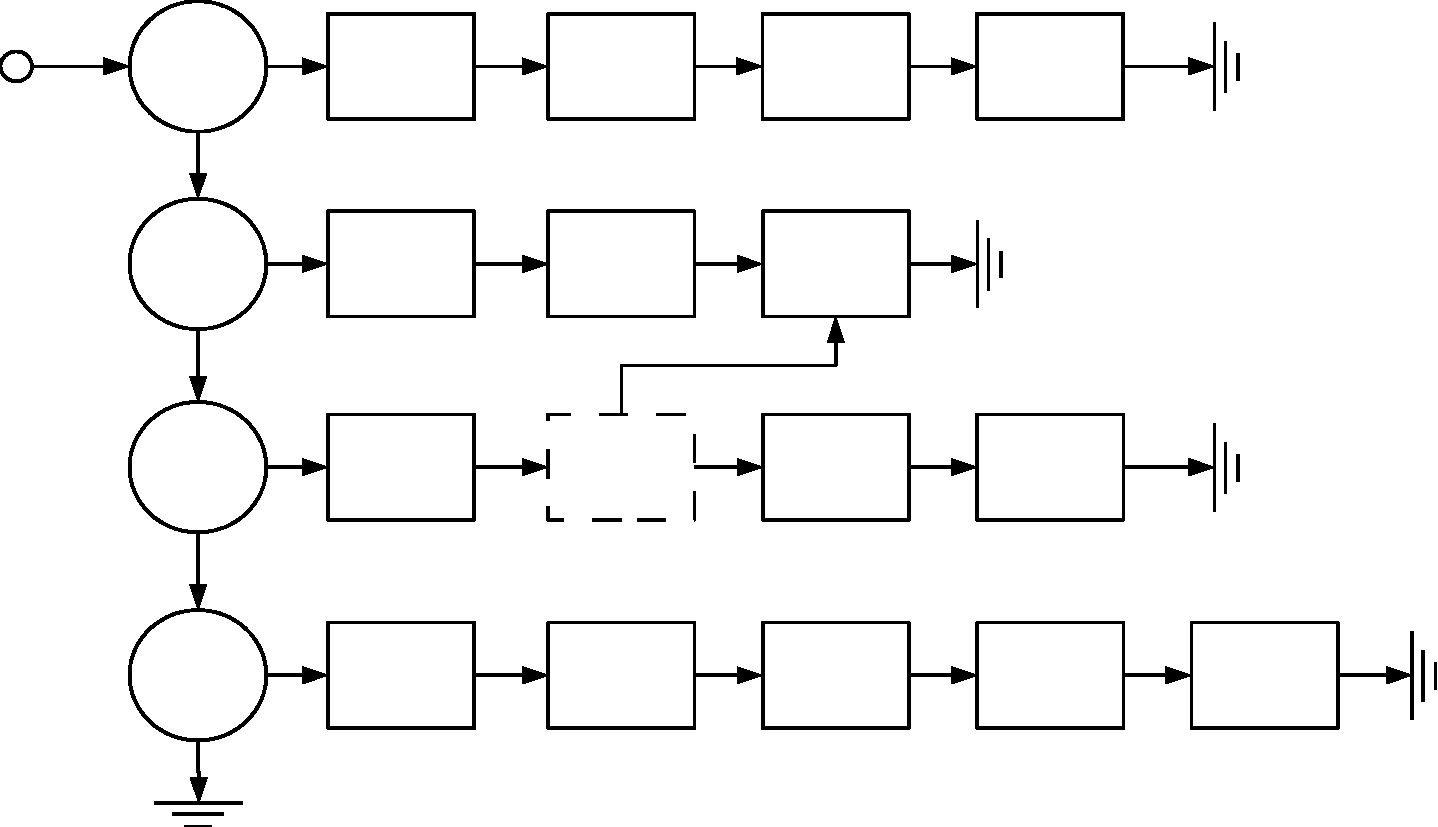
\includegraphics[width=0.7\textwidth]{channel_logo}}\\[9mm]
  {\huge\bf Patrick J\"ockel$^{1,2}$, Astrid Kerkweg{$^3$},}\\[3mm]
  {\huge\bf Andrea Pozzer$^4$, Rolf Sander$^1$, Holger Tost$^1$,}\\[3mm]
  {\huge\bf Hella Riede$^1$, Andreas Baumgaertner$^1$,}\\[3mm]
  {\huge\bf Sergey Gromov$^1$, Bastian Kern$^1$}\\[9mm]
  \Large
  $^1$ Air Chemistry Department, Max-Planck Institute of Chemistry,
       PO Box 3060, 55020 Mainz, Germany\\
  $^2$ Deutsches Zentrum f\"{u}r Luft- und Raumfahrt, Institut
       f\"{u}r Physik der Atmosph\"{a}re, Oberpfaffenhofen, 82230 Wessling,
       Germany\\
  $^3$ Institute for Atmospheric Physics, University Mainz, 55128 Mainz,
       Germany\\
  $^4$ Cyprus Institute, EEWRC, P.O. Box 27456, 1645 Nicosia, Cyprus\\
  \url{Patrick.Joeckel@dlr.de}

\end{center}

\vfill

{\large This manual is part of the electronic supplement of our article
``Development Cycle 2 of the Modular Earth Submodel System (MESSy2)''
  in Geosci.\ Model\ Dev.\
  (2010), available at: \url{http://www.geoscientific-model-development.net}}

\begin{center}
%  Date: \thedate
  Date: \today
\end{center}

\newpage
\tableofcontents
\newpage

%%%%%%%%%%%%%%%%%%%%%%%%%%%%%%%%%%%%%%%%%%%%%%%%%%%%%%%%%%%%%%%%%%%%%%%%%%%%%%
%% ###########################################################################
%%%%%%%%%%%%%%%%%%%%%%%%%%%%%%%%%%%%%%%%%%%%%%%%%%%%%%%%%%%%%%%%%%%%%%%%%%%%%%
\section{Introduction}
%%%%%%%%%%%%%%%%%%%%%%%%%%%%%%%%%%%%%%%%%%%%%%%%%%%%%%%%%%%%%%%%%%%%%%%%%%%%%%
%% ###########################################################################
%%%%%%%%%%%%%%%%%%%%%%%%%%%%%%%%%%%%%%%%%%%%%%%%%%%%%%%%%%%%%%%%%%%%%%%%%%%%%%
%
This document describes some more details of the MESSy infrastructure
submodel CHANNEL for the coupling of processes in Earth System Models.
%
CHANNEL provides the application programming interface (API) of a comfortable
and powerful memory management, suitable for the flexible and efficient data
exchange / data sharing between different processes (submodels). CHANNEL
further serves the input / output of data from / into files, entirely
controllable via namelists. The implemented features comprise
\begin{itemize}
 \item a full input / output control (user interface) via Fortran95 namelists,
 \item a powerful restart facility for simulation chains,
 \item output redirection for tailor made output files,
 \item a flexible choice of the output file format, the output method and the
       output precision, and
 \item the capability to conduct basic statistical analyses w.r.t.\ time
       on-line, i.e., to output in addition (or alternative) to the
       instantaneous data the average, standard deviation, minimum, maximum,
       event counts, and event averages.
\end{itemize}
%
For the application of a base model, which contains already the
CHANNEL infrastructure, the user interface (namelist control)
is explained in Sect.~\ref{sec:channelui}.

All other sections provide a reference for the
implementation of the CHANNEL infrastructure into new basemodels
(in particular Sects.~\ref{sec:error}, \ref{sec:channelbmil},
\ref{sec:cat} and {\ref{sec:messymainchannelother}),
and for the application of the CHANNEL infrastructure in submodels, when the
basemodel already contains the CHANNEL infrastructure.

CHANNEL is written in Fortran95 (ISO/IEC-1539-1) following an object oriented
approach to the extent possible. The basic entities (implemented as Fortran95
structures) in CHANNEL are
\begin{itemize}
 \item {\it attributes}, $\rightarrow$ time independent, scalar
       characteristics,
 \item {\it dimension variables}, $\rightarrow$ specific coordinate axes,
 \item {\it dimensions}, $\rightarrow$ the basic geometry in one dimension
 \item {\it representations}, $\rightarrow$ multidimensional geometric
       structures (based on {\it dimensions}),
 \item {\it channel objects}, $\rightarrow$ data fields including their meta
       information ({\it attributes}) and their underlying geometric
       structure ({\it representation})
 \item {\it channels}, $\rightarrow$ sets of ``related''
       {\it channel objects} with additional meta information.
       The ``relation'' can be, for instance, the simple fact that the
       {\it channel objects} are defined by the same submodel.
\end{itemize}
%
These structures are explained in more detail in Sect.~\ref{sec:types} for
reference. Direct access to the structures is not required, since
CHANNEL provides a powerful application programming interface (API),
as explained in Sects.~\ref{sec:error} and \ref{sec:be}.
The specific coupling of the MESSy infrastructure submodel TRACER to
CHANNEL is explained in Sect.~\ref{sec:cat}.

For data input / output,
currently interfaces for
netCDF\footnote{\url{http://www.unidata.ucar.edu/software/netcdf}}
and
parallel netCDF\footnote{\url{http://www.mcs.anl.gov/parallel-netcdf}}
are implemented, the implementation of
alternative file formats is straightforward due to the modular
structure of CHANNEL.
This is further explained in Sect.~\ref{sec:io}.

%%%%%%%%%%%%%%%%%%%%%%%%%%%%%%%%%%%%%%%%%%%%%%%%%%%%%%%%%%%%%%%%%%%%%%%%%%%%%%
%% ###########################################################################
%%%%%%%%%%%%%%%%%%%%%%%%%%%%%%%%%%%%%%%%%%%%%%%%%%%%%%%%%%%%%%%%%%%%%%%%%%%%%%
\section{CHANNEL namelist user interface}
\label{sec:channelui}
%%%%%%%%%%%%%%%%%%%%%%%%%%%%%%%%%%%%%%%%%%%%%%%%%%%%%%%%%%%%%%%%%%%%%%%%%%%%%%
%% ###########################################################################
%%%%%%%%%%%%%%%%%%%%%%%%%%%%%%%%%%%%%%%%%%%%%%%%%%%%%%%%%%%%%%%%%%%%%%%%%%%%%%
According to the MESSy standard
\citep{442}\footnote{\url{http://www.atmos-chem-phys.net/8/1677}},
the user interface of the submodel CHANNEL
is subdivided into a control ({\tt CTRL}) and a coupling ({\tt CPL}) namelist,
where the latter contains base model specific control parameters and
a coupling to the MESSy infrastructure submodel TIMER for the time control
of output files.
Both namelists are contained in the namelist file {\it channel.nml}.

%%%%%%%%%%%%%%%%%%%%%%%%%%%%%%%%%%%%%%%%%%%%%%%%%%%%%%%%%%%%%%%%%%%%%%%%%%%%%%
\subsection{CHANNEL CTRL namelist}
\label{sec:channelCTRL}
%%%%%%%%%%%%%%%%%%%%%%%%%%%%%%%%%%%%%%%%%%%%%%%%%%%%%%%%%%%%%%%%%%%%%%%%%%%%%%
The {\tt CTRL} namelist comprises entries to control the output and restart
handling for all {\it channels} and {\it channel objects}.
An example is given in Figure~\ref{fig:channel_ctrl}.
%
\begin{figure}[h!]
\begin{center}
\begin{minipage}{0.6\textwidth}
\footnotesize
\begin{verbatim}
&CTRL
!
EXP_NAME='test'       ! EXPERIMENT NAME
EXEC_CHECKSUM='$EXEC_CHECKSUM',
! ---------------------------------------------------------------------
!
L_FLUSH_IOBUFFER = F, ! FLUSH I/O BUFFER IN EVERY TIME STEP
                      ! (DEFAULT: T (true))
! ---------------------------------------------------------------------
! # OUTPUT TO LOG-FILE
! #  0: only error
! #  1: initialze and finalize
! #  2: 1 and time loop  (default)
! #  3: additional debug output
I_VERBOSE_LEVEL = 1,
! ---------------------------------------------------------------------
!
OUT_PREC  = 1, 1, 1, 1, 1, 1,  ! OUTPUT PRECISION (production)
!OUT_PREC = 1, 2, 2, 1, 1, 1,  ! OUTPUT PRECISION (for tests)
!
! # SET DEFAULT OUTPUT AND RESTART HANDLING
!      - '', OUTPUT-FILETYPE, RERUN-FILETYPE,
!        NO. OF STEPS PER OUTPUT-FILE, RERUN, IGNORE,
!        INST, AVE, STD, MIN, MAX, CNT, CAV, RANGE(2)
!
OUT_DEFAULT = '', 3, 3, -1, F,F, T,F,F,F,F, F,F, , ,
!
! ---------------------------------------------------------------------
! # ADD NEW OUTPUT CHANNELS
ADD_CHANNEL(1)   = 'special',
ADD_CHANNEL(2)   = 'carbon',
!
! ---------------------------------------------------------------------
! # ADD NEW CHANNEL OBJECT REFERENCES
!   NOTES:
!    - SOURCE OBJECT NAME MAY CONTAIN WILDCARDS '?' AND '*'
!      (in this case, target object name is ignored)
!    - TARGET CHANNEL NAME MAY CONTAIN WILDCARDS '?' AND '*'
!    - TARGET OBJECT NAME SET TO SOURCE OBJECT NAME, IF ''
!
ADD_REF(1) = 'g3b',      'aps',    '*',         '',
ADD_REF(2) = 'g3b',      'geopot', 'tracer_gp', 'geop',
ADD_REF(3) = 'tracer_gp','C*',     'carbon',    '',
!
! ---------------------------------------------------------------------
! # SET CHANNEL SPECIFIC DEFAULT OUTPUT AND RESTART HANDLING
!      - channel-name, OUTPUT-FILETYPE, RERUN-FILETYPE,
!        NO. OF STEPS PER OUTPUT-FILE, RERUN, IGNORE,
!        INST, AVE, STD, MIN, MAX, CNT, CAV, RANGE(2)
!   NOTE: IF NO. OF STEPS PER OUTPUT-FILE <= 0,
!         THE EVENT TRIGGER (CPL-NAMELIST, TIMER_TNF BELOW)
!         CONTROLS THE FILE CONTENT
!
OUT_CHANNEL(1) = 'g3b',    3, 3, 10, F,F, T,F,F,F,F, F,F, , ,
OUT_CHANNEL(2) = 'qtimer', 3, 3, -1, F,F, T,T,T,T,T, F,F, , ,
OUT_CHANNEL(3) = 'special',3, 3, -1, F,F, F,T,F,F,F, F,F, , ,
!
! ---------------------------------------------------------------------
! # SET CHANNEL OBJECT SPECIFIC OUTPUT AND RESTART HANDLING
!      - channel-name, object-name, RERUN, IGNORE,
!        INST, AVE, STD, MIN, MAX, CNT, CAV, RANGE(2)
!
OUT_OBJECT(1)  = 'g3b',   'aps',     F,F, T,F,F,F,F, F,F, , ,
OUT_OBJECT(2)  = 'carbon','C2H4',    F,T, T,T,F,F,F, F,F, , ,
/
\end{verbatim}
\end{minipage}
\end{center}
\caption{Example CTRL namelist of the generic submodel CHANNEL.
For explanations, see text.}
 \label{fig:channel_ctrl}
\end{figure}
%

Four entries control the overall output:
%
\begin{itemize}
 \item {\tt EXP\_NAME} is an arbitrary string (of maximum 15 characters)
       which defines the simulation.
       This string (padded with trailing underscores) represents the first
       part of the output filenames, followed by an underscore.
       The output filename is completed by the simulation date and time
       (format {\tt YYYYMMDD\_hhmm}) of the first entry in the file, another
       underscore, the name of the {\it channel}, and the file format
       specific extension (including the dot), in summary
       {\tt {\it EXP\_NAME}\_YYYYMMDD\_hhmm\_{\it channel.ext}}.\\
       Example: {\tt EXP\_NAME = 'test',}\\
       results for instance in the netCDF ({\tt .nc}) filename
       \verb|test____________20090101_0030_tracer_gp.nc|
%       {\tt test\_\_\_\_\_\_\_\_\_\_\_\_20090101\_0030\_tracer\_gp.nc}
       for the {\it channel} {\tt tracer\_gp}.
       The first output time step in this file corresponds to the simulation
       time January 1, 2009 at 00:30 UTC.
 \item {\tt L\_FLUSH\_IOBUFFER} is a logical switch, which controls the
       flushing
       of the output memory buffers. If set to {\tt T} (default) the output
       buffers of all output files are flushed at the end of each output
       time step, otherwise ({\tt F}) the flushing is determined by the
       runtime environment (i.e., if the buffer is full). For instance,
       if netCDF
       is used as output format, flushing every output time step
       might reduce the overall runtime performance, however, it guarantees
       valid files even after a crash of the simulation.\\
       Example: {\tt L\_FLUSH\_IOBUFFER = T,}
 \item {\tt OUT\_PREC} is a one dimensional array of length 6 for setting
       the output precision for the output file formats
       (ASCII, parallel netCDF, netCDF, GRIB, HDF4, HDF5), respectively.
       Currently only netCDF and parallel netCDF are implemented.
       For netCDF and parallel netCDF, {\bf 1} sets the output to
       {\tt NF90\_FLOAT}
       and {\bf 2} to {\tt NF90\_DOUBLE}, respectively.
       Output in double precision is helpful
       for performing restart-tests, i.e., for checking that the simulation
       results are independent of the chosen restart frequency in
       simulation chains.\\
       Example: {\tt OUT\_PREC = 1,2,1,1,1,1,}
 \item {\tt OUT\_DEFAULT} is a structure controlling the default output
       settings of all {\it channels} and {\it channel objects};
       the elements are
       \begin{enumerate}
        \item an empty string (this string is used for {\it channel} specific
              settings (see {\tt OUT\_CHANNEL} below),
        \item an integer to control the output file-type (currently only
              parallel netCDF (2) and netCDF (3) are implemented),
        \item an integer to control the restart file-type (currently only
              parallel netCDF (2) and netCDF (3) are implemented),
        \item an integer to control the maximum number of time-steps
              per output file (if this number is reached, a new output-file
              is started),
        \item a logical to force output into the restart file,
        \item a logical to ignore, if an object is not present in a restart
              file, although required (this is useful if additional submodels
              are switched on after a restart),
        \item a logical to output instantaneous data (i.e., the values at
              the output time step, INST),
        \item a logical to output the average w.r.t.\ time
              of the data between two subsequent output time steps (AVE),
        \item a logical to output the standard deviation w.r.t.\ time
              of the data between two subsequent output time steps (STD),
        \item a logical to output the minimum w.r.t.\ time
              of the data between two subsequent output time steps (MIN),
        \item a logical to output the maximum w.r.t.\ time
              of the data between two subsequent output time steps (MAX),
        \item a logical to count (and output) the number of events
              defined by the data being within a specific range
              between two subsequent output time steps (CNT),
        \item a logical to average over the events defined by the data
              being within a specific range
              between two subsequent output time steps (CAV),
        \item a pair of real numbers describing the interval boundaries
              for CNT and CAV, the defaults are
              {\tt -HUGE(0.0\_DP)} and {\tt HUGE(0.0\_DP)}, respectively.
       \end{enumerate}
       The corresponding variable names in the output (and restart) files
       are the {\it channel object} names extended by an underscore and the
       suffixes (in lowercase) listed in parentheses, except for INST,
       for which no extension is used.\\
       Example: {\tt OUT\_DEFAULT = '', 2, 2, 10, F,F, T,F,F,F,F, F,F, , ,}\\
       specifies parallel netCDF output as file-type for output ({\tt 2}) and
       restart files ({\tt 2}), respectively; a maximum of {\tt 10} output
       time steps are written to each output file. The objects without
       {\tt lrestreq=.TRUE.} (see Sects.~\ref{sec:chanobj},
       \ref{par:newchannel} and \ref{par:newchannelobject}) set in the code
       are not written to the restart files ({\tt F}). After a restart
       {\it channel objects} with {\tt lrestreq=.TRUE.} which are not present
       in the respective restart file will not be ignored ({\tt F}), but
       rather cause an error. The instantatneous data of the
       {\it channel objects} are output ({\tt T}), but none of the
       derived statistics ({\tt F,F,F,F, F,F}). The standard range for the
       conditional statisitcs (CNT and CAV) remains default ({\tt  , ,}).
\end{itemize}

The settings in {\tt OUT\_DEFAULT} can be overwritten for specific
{\it channels} and / or specific {\it channel objects}, respectively:
\begin{itemize}
 \item {\tt OUT\_CHANNEL(n)} is used for {\it channels}, where
       {\it n} is an arbitrary but unique number between 1 and 500.
       The same entries (1-14) as in {\tt OUT\_DEFAULT} are used, but
       the empty string (entry 1) is replaced by the name of the
       {\it channel}.\\
       Example: {\tt OUT\_CHANNEL(1) = 'geoloc', 2, 2, 10, F,F, F,F,F,F,F, F,F, , ,}
 \item {\tt OUT\_OBJECT(n)} is used for {\it channel objects}, where
       {\it n} is an arbitrary but unique number between 1 and 1000.
       The entries correspond to the entries 5-14 of {\tt OUT\_DEFAULT},
       preceded by two strings denoting the name of the {\it channel} and the
       name of the {\it channel object}, respectively.\\
       Example: {\tt OUT\_OBJECT(1) = 'g3b','qtnew', F,F, F,F,F,F,F, F,F, , ,}
\end{itemize}

In a standard setup, all {\it channel objects} in a specific {\it channel},
which are subject to output (i.e., for which not all of the output flags
above (entries 7-13) are {\tt F}),
are written to the same output file. The possibility exists,
however, to re-direct the output of {\it channel objects} into different
output files by creating {\it channel object references} in the namelist with
the variable
\begin{itemize}
 \item {\tt ADD\_REF(n)}, where {\it n} denotes an arbitrary but unique
 number between 1 and 500 and each {\it reference} consists of four strings
 denoting
  \begin{itemize}
  \item the name of the original {\it channel} which contains the
        {\it channel object} to be referenced,
  \item the name of the {\it channel object} to be referenced,
  \item the name of the target {\it channel}, i.e., the {\it channel}
        the object should be referenced from,
  \item the name of the {\it channel object} in the referencing {\it channel}.
        If this entry is empty, the original name of the {\it channel object}
        is used.
  \end{itemize}
  Example: {\tt ADD\_REF(1) = 'g3b', 'aps', 'tracer\_gp', 'ps',}\\
  creates in {\it channel} {\tt tracer\_gp} a reference (with name {\tt ps},
  to the {\it channel object} {\tt aps} of {\it channel} {\tt g3b}.
\end{itemize}
%
A special feature is that the name of the target {\it channel} can contain
wildcards ('*' or '?'). The {\it channel object reference} is then created
in every {\it channel} with matching name. For example\\
{\tt ADD\_REF(1) = 'g3b', 'aps', '*', '',}\\
creates in every {\it channel} ({\tt *}) a reference (with name {\tt aps},
since the last string is empty, {\tt ''}) to the {\it channel object}
{\tt aps} of {\it channel} {\tt g3b}.

Also the name of the {\it channel object} to be referenced can contain
wildcards ('*' or '?'). In this case, all matching {\it channel objects}
from the original {\it channel} will be referenced from the target
{\it channel} -- with the name of the original {\it channel object}.
This implies that in this case, a potentially
specified {\it channel object} name in the referencing {\it channel}
(4th entry) is ignored. For example\\
{\tt ADD\_REF(2) = 'tracer\_gp', 'C*', 'carbon', '',}\\
creates in the {\tt carbon} {\it channel} references for all
{\it channel objects} of the {\tt tracer\_gp} {\it channel} which names start
with 'C'.

The {\it channel object reference}(s) share(s)
with the original {\it channel object} the memory for the primary data,
i.e., no additional memory is consumed. Memory for secondary
(derived statistical) data, however, is created for each
{\it channel object reference} as it is requested by the corresponding
namelist entries
({\tt OUT\_DEFAULT}, {\tt OUT\_CHANNEL(n)}, {\tt OUT\_OBJECT(n)}).
This additional memory is required to allow independent output time intervals
and statistics for the {\it channel object reference}(s)}.

In addition to the creation of {\it channel object references} for
output redirection into other already existing {\it channels},
also new channels can be created with the namelist variable
%
\begin{itemize}
 \item {\tt ADD\_CHANNEL(n)}, where {\it n} denotes an arbitrary but unique
 number between 1 and 50, and each new {\it channel} is specified by its
 unique name.\\
 Example: {\tt ADD\_CHANNEL(1) = 'special',}
\end{itemize}

As indicated above
(entry 4 of {\tt OUT\_DEFAULT} and / or {\tt OUT\_CHANNEL(n)}),
the size of the output files is controlled via the maximum
number of time steps per file.
If this number is set to zero or
negative, the files are controlled via the entries in the {\tt CPL} namelist
as described in the next section.

Last but not least, the {\tt \&CTRL} namelist contains two additional entries:
\begin{itemize}
\item {\tt EXEC\_CHECKSUM} contains the checksum of the executable used. It is
  automatically set by the runscript and helps to identify the
  executable used for a specific simulation.
\item {\tt I\_VERBOSE\_LEVEL} controls the output to the log-file. While
  values of \verb|0-2| switch in which parts of the simulation (0: none, 1:
  initial phase, 2: initial phase and time loop) additional output is written,
  numbers $>2$ trigger additional debug output: e.g. \verb|I_VERBOSE_LEVEL= 3|
  writes out the channel object name each time \verb|get_channel_object| is
  called. This may help, to find the missing/wrongly named object, if the
  simulation is terminated with the error message
  \verb|'CHANNEL OBJECT DOES NOT EXIST'|.
\end{itemize}
%%%%%%%%%%%%%%%%%%%%%%%%%%%%%%%%%%%%%%%%%%%%%%%%%%%%%%%%%%%%%%%%%%%%%%%%%%%%%%
\subsection{CHANNEL CPL namelist}
\label{sec:channelCPL}
%%%%%%%%%%%%%%%%%%%%%%%%%%%%%%%%%%%%%%%%%%%%%%%%%%%%%%%%%%%%%%%%%%%%%%%%%%%%%%
%
An example for the {\tt CPL} namelist of CHANNEL is given in
Figure~\ref{fig:channel_cpl}.
%

\begin{figure}[h!]
\begin{center}
\begin{minipage}{0.6\textwidth}
\footnotesize
\begin{verbatim}
&CPL
!
L_BM_ORIG_OUTPUT = F, ! ENABLE ORIGINAL LEGACY MODEL OUTPUT ?
!
! # SET OUTPUT INTERVALS FOR ALL CHANNELS (DEFAULT + INDIVIDUAL)
!   NOTE: First match (wildcard) counts!
!
TIMER_DEFAULT    = '',     5, 'hours',   'first', 0,
!
TIMER_CHANNEL( 1) = 'qtimer',  1, 'steps',   'first', 0,
TIMER_CHANNEL( 2) = 'scout',   1, 'hours',   'first', 0,
TIMER_CHANNEL( 3) = 'special', 1, 'months',  'first', 0,
!
! # SET TIMER EVENTS FOR NEW FILENAMES
!   (IF NO. OF STEPS PER OUTPUT-FILE <= 0 ABOVE !!!)
!   NOTE: First match (wildcard) counts!
!
TIMER_TNF_DEFAULT = '', 1, 'days', 'first', 0,
!
TIMER_TNF_CHANNEL( 1) = 'qtimer', 1, 'days',   'first', 0
TIMER_TNF_CHANNEL( 2) = 'scout*', 1, 'months', 'first', 0
!
/
\end{verbatim}
\end{minipage}
\end{center}
\caption{Example CPL namelist of the generic submodel CHANNEL.
For explanations, see text.}%
\label{fig:channel_cpl}
\end{figure}
%

The {\tt CPL} namelist
of CHANNEL provides the switch {\tt L\_BM\_ORIG\_OUTPUT}
(default {\tt F}) to enable ({\tt T}) the original output of the basemodel,
in case the base model supports this.

The more important features, however, are provided by a coupling to the
MESSy infrastructure submodel TIMER. This enables the control of the
output frequency and the file sequence containing a time series.

The default output frequency for all {\it channels} is set by the variable
{\tt TIMER\_DEFAULT}, which can be overwritten for each {\it channel} by
the variable {\tt TIMER\_CHANNEL(n)}, where {\it n} indicates an arbitrary
but unique number between 1 and 500. The frequency to create new files
is set by the variable {\tt TIMER\_TNF\_DEFAULT} (default) for all
{\it channels}, and overwritten for specific {\it channels} by the
variable {\tt TIMER\_TNF\_CHANNEL(n)}, respectively. Also here {\it n}
denotes an arbitrary but unique number between 1 and 500.

All four variables consist of
\begin{itemize}
 \item the name of the {\it channel}, which is empty for the
       DEFAULT variables,
 \item an event trigger, which consists of
       \begin{itemize}
        \item the length of the time interval (integer),
        \item the unit of the time interval (string), e.g.,
              'steps', 'minutes', 'hours', 'days', 'months', 'years',
        \item the positioning of the triggering time step in the given
              interval, i.e., 'first', 'last', or 'exact',
        \item an offset in seconds (integer), which is usually zero.
       \end{itemize}
\end{itemize}
%
As an example, the namelist entry
\begin{verbatim}
  TIMER_CHANNEL( 1) = 'g3b', 5, 'hours', 'first', 0
\end{verbatim}
triggers the output of all {\it channel objects} in the {\it channel}
'g3b', for which output is requested, at the 'first' time step in every
5 hours with no offset.
%
The entry
\begin{verbatim}
  TIMER_TNF_DEFAULT = '', 1, 'days', 'first', 0,
\end{verbatim}
triggers a new file creation per default for all {\it channels} at the
'first' time step of every day without offset.

This feature for controlling new file creation is only active, however,
for those channels, for which the
number of time steps per output file in the {\tt CTRL} namelist
(entry 4 of {\tt OUT\_DEFAULT} and / or {\tt OUT\_CHANNEL(n)}) is set to zero
or negative.

%%%%%%%%%%%%%%%%%%%%%%%%%%%%%%%%%%%%%%%%%%%%%%%%%%%%%%%%%%%%%%%%%%%%%%%%%%%%%%
\subsection{CHANNEL CTRL\_PNETCDF namelist}
\label{sec:channelCTRLPNETCDF}
%%%%%%%%%%%%%%%%%%%%%%%%%%%%%%%%%%%%%%%%%%%%%%%%%%%%%%%%%%%%%%%%%%%%%%%%%%%%%%
The {\tt CTRL\_PNETCDF} namelist comprises entries to tune the
performance of the parallel netCDF output via
MPI-IO hints in the form {\tt MPI\_IO\_HINT(n) = hint,value}
where {\it n} denotes an arbitrary but unique number between 1 and 10,
{\it hint} is the name of the MPI-IO hint, and {\it value} its value.
Example:
\begin{verbatim}
&CTRL_PNETCDF
  MPI_IO_HINT(1) = 'IBM_sparse_access','true',
/
\end{verbatim}

%%%%%%%%%%%%%%%%%%%%%%%%%%%%%%%%%%%%%%%%%%%%%%%%%%%%%%%%%%%%%%%%%%%%%%%%%%%%%%
%% ###########################################################################
%%%%%%%%%%%%%%%%%%%%%%%%%%%%%%%%%%%%%%%%%%%%%%%%%%%%%%%%%%%%%%%%%%%%%%%%%%%%%%
\section{Type definitions of basic entities}
\label{sec:types}
%%%%%%%%%%%%%%%%%%%%%%%%%%%%%%%%%%%%%%%%%%%%%%%%%%%%%%%%%%%%%%%%%%%%%%%%%%%%%%
%% ###########################################################################
%%%%%%%%%%%%%%%%%%%%%%%%%%%%%%%%%%%%%%%%%%%%%%%%%%%%%%%%%%%%%%%%%%%%%%%%%%%%%%
The basic entities used within the MESSy CHANNEL infrastructure submodel are
\begin{itemize}
 \item {\it attributes},
 \item {\it dimension variables},
 \item {\it dimensions},
 \item {\it representations},
 \item {\it channel objects},
 \item {\it channels}.
\end{itemize}
%
These entities are hierarchically organised in a way that a higher entity
(later in list) can make use of a lower entity (earlier in list).
%
This section provides a complete reference of the corresponding Fortran95
structures. It is important to note that the application of the MESSy submodel
CHANNEL does not require any direct access to these structures in the code.
Application of the submodel CHANNEL is possible by exclusive usage of the
interface subroutines which are explained in the subsequent sections.

Figure~\ref{fig:channelmodules} sketches the relationship between
the different entities and the corresponding Fortran95 modules.
%
\begin{figure}
  \centerline{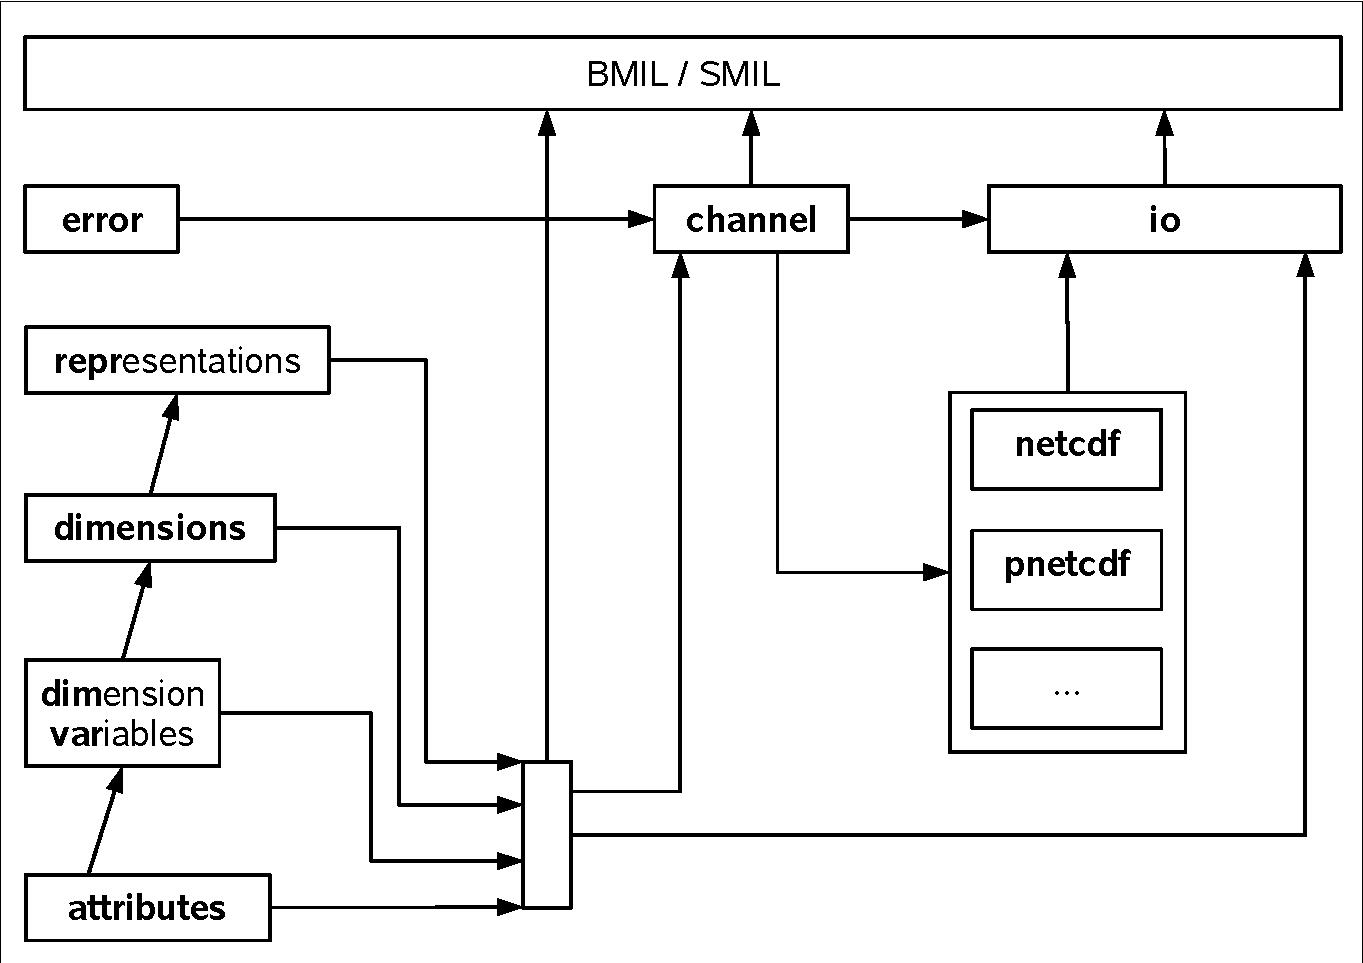
\includegraphics[width=0.7\textwidth]{channel_modules}}
  \caption[Relationship between channel entities and modules]
          {Relationship between the various channel entities and Fortran95
          modules: The boxes represent the different Fortran95 modules of
          CHANNEL, the corresponding filenames are
          {\tt messy\_main\_channel\_{\it bf.f90}}, where {\it bf} is the
          respective bold-face text. The arrows indicate where the different
          modules are {\tt USE}d. Different output formats / methods
          (netcdf, pnetcdf (for parallel-netCDf), and other formats / methods
          indicated by the dots) are summarised in a common box for the sake of
          readability to reduce the number of arrows. Similarly, the empty
          box summarises similar uses of the connected modules.
          BMIL and SMIL denote the basemodel layer and the submodel interface
          layer, respectively.}
  \label{fig:channelmodules}
\end{figure}
%

Fortran parameters defined in {\tt messy\_main\_constants\_mem.f90} used
for the type declarations are:
\begin{verbatim}
  ! PRECISION SETTINGS
  INTEGER, PARAMETER :: DP = SELECTED_REAL_KIND(12,307)
  INTEGER, PARAMETER :: I8 = SELECTED_INT_KIND(14)

  ! STRING LENGTHs
  INTEGER, PARAMETER :: STRLEN_SHORT  = 8
  INTEGER, PARAMETER :: STRLEN_MEDIUM = 24
  INTEGER, PARAMETER :: STRLEN_LONG   = 64
  INTEGER, PARAMETER :: STRLEN_VLONG  = 80
  INTEGER, PARAMETER :: STRLEN_ULONG  = 256
\end{verbatim}

%
% attributes
\subsection{Attributes}
\label{sec:att}
An {\it attribute} describes a time independent, scalar
characteristic of a higher entity.
The information is stored in a Fortran95 structure:

\begin{verbatim}
  TYPE t_attribute
     CHARACTER(LEN=STRLEN_MEDIUM) :: name    = ''
     INTEGER                      :: type    = TYPE_UNKNOWN
     INTEGER                      :: iflag   = AF_NONE
     INTEGER                      :: i = 0
     CHARACTER(LEN=STRLEN_ULONG)  :: c = ''
     REAL(DP)                     :: r = 0.0_DP
  END TYPE t_attribute
\end{verbatim}

{\it Attributes} are identified by their {\tt name} and are of a unique
{\tt type} (pre-defined with the Fortran95 parameter {\tt TYPE\_UNKNOWN}),
which is either {\tt INTEGER} (parameter {\tt TYPE\_INTEGER}),
{\tt REAL(DP)} (parameter {\tt TYPE\_REAL\_DP}) or\\
{\tt CHARACTER(LEN=STRLEN\_ULONG)} (parameter {\tt TYPE\_STRING}).
A set of attributes of a higher entity is stored in a concatenated list
of attributes:

\begin{verbatim}
  TYPE t_attribute_list
     TYPE(t_attribute)               :: this
     TYPE(t_attribute_list), POINTER :: next => NULL()
  END TYPE t_attribute_list
\end{verbatim}

Basic subroutines for managing {\it attributes} and {\it attribute lists}
are contained in the Fortran95 module\\
{\tt messy\_main\_channel\_attributes.f90}
(Sect.~\ref{sec:messymainchannelattributes}).
The Fortran95 module {\tt messy\_main\_channel.f90}
(Sect.~\ref{sec:messymainchannel}) contains additional subroutines for
handling {\it attribute lists} of higher entities.

% dimension variables
\subsection{Dimension variables}
\label{sec:dimvar}

A {\it dimension variable} contains the information of a discrete coordinate,
such as an axis of a spatial dimension (e.g., latitude). The required
information is stored in a Fortran95 structure:

\begin{verbatim}
  TYPE t_dimvar
     CHARACTER(LEN=STRLEN_MEDIUM)    :: name  = ''    ! NAME OF VARIABLE
     REAL(DP), DIMENSION(:), POINTER :: val => NULL() ! VALUES
     TYPE(t_attribute_list), POINTER :: att => NULL() ! ATTRIBUTE LIST
  END TYPE t_dimvar
\end{verbatim}

Each {\it dimension variable} is identified by its {\tt name}. The
coordinate values are stored in the array {\tt val}. The {\it attribute list}
contains further information, such as for instance the unit of the coordinate
values (e.g., ``unit''=''degrees\_north'' for the latitude).

{\it Dimension variables} are necessarily associated with {\it dimensions}
(Sect.~\ref{sec:dim}). Since more than one {\it dimension variable} can be
associated with a specific {\it dimension}, lists of
{\it dimension variables} are stored in a concatenated Fortran95 structure:

\begin{verbatim}
  TYPE t_dimvar_list
     TYPE(t_dimvar)               :: this
     TYPE(t_dimvar_list), POINTER :: next => NULL()
  END TYPE t_dimvar_list
\end{verbatim}

Subroutines for managing {\it dimension variables} and
{\it dimension variable lists} are contained in the Fortran95
module {\tt messy\_main\_channel\_dimvar.f90}
(Sect.~\ref{sec:messymainchanneldimvar}).

% dimensions
\subsection{Dimensions}
\label{sec:dim}

The term {\it dimension} is self-explanatory. The structure is:
%
\begin{verbatim}
    TYPE t_dimension
     CHARACTER(LEN=STRLEN_MEDIUM) :: name  = ''          ! NAME OF DIMENSION
     INTEGER                      :: id    = DIMID_UNDEF ! ID OF DIMENSION
     INTEGER                      :: len   = 0           ! LENGTH OF DIMENSION
     LOGICAL                      :: ltime = .FALSE.     ! FLAG FOR TIME DIM.
     TYPE(t_dimvar_list), POINTER :: var   => NULL()     ! DIMENSION VARIABLES
  END TYPE t_dimension
\end{verbatim}
%
A {\it dimension} is identified by its unique {\tt name} and identifier
({\tt id}). The basic information hold by a {\it dimension} is its
length ({\tt len}), which is the number of discrete steps along the axis.
A special flag is used to indicate
that the {\it dimension} is the time dimension ({\tt ltime}).
Specific coordinate
values may be stored in a list of {\it dimension variables}
({\tt var}, Sect.~\ref{sec:dimvar}).

All {\it dimensions} are stored internally in one list.
Subroutines for managing {\it dimensions} are contained in the Fortran95
module {\tt messy\_main\_channel\_dimensions.f90}
(Sect.~\ref{sec:messymainchanneldimensions}).

% representations
\subsection{Representations}
\label{sec:repr}

A {\it representation} describes the underlying geometric structure of data.
The required information is stored in a Fortran95 structure:

\begin{verbatim}
  TYPE t_representation
     ! IDENTIFICATION
     CHARACTER(LEN=STRLEN_MEDIUM) :: name    = ''    ! NAME
     INTEGER                      :: id      = 0     ! ID
     INTEGER                      :: rank    = 0     ! RANK
     CHARACTER(LEN=IRANK)         :: link    = ''    ! LINK-STRING
     CHARACTER(LEN=IRANK)         :: axis    = ''    ! AXIS-STRING
     INTEGER, DIMENSION(IRANK)    :: gdimlen = 0     ! GLOBAL DIMENSION LENGTH
     !
     ! DECOMPOSITION INFORMATION
     INTEGER, DIMENSION(IRANK)    :: ldimlen = 0     ! LOCAL DIMENSION LENGHT (ON THIS PE)
     INTEGER                      :: dctype  = 0     ! DECOMPOSTION TYPE
     !
     ! FULL DIMENSION INFORMATION (POINTER TO DIMENSION; GLOBAL !!!)
     TYPE(t_dimension_ptr), DIMENSION(IRANK) :: dim
     !
     ! INPUT/OUTPUT CONVERSION
     ! - PERMUTATION OF DIMENSIONS BEFORE OUTPUT
     LOGICAL                   :: lperm          = .FALSE.
     INTEGER, DIMENSION(IRANK) :: order_mem2out  = 0 ! output
     INTEGER, DIMENSION(IRANK) :: shape_out      = 0 ! shape in output
     INTEGER, DIMENSION(IRANK) :: order_out2mem  = 0 ! input
     !
     ! BOUNDARY MEMORY MANAGEMENT
     TYPE(t_repr_boundary)    :: bounds
     !
     ! PARALLEL DECOMPOSITION INFORMATION
     TYPE(t_repr_pdecomp)      :: pdecomp
     !
  END TYPE t_representation
\end{verbatim}

Each {\it representation} is identified by a unique {\tt name} and identifier
({\tt id}). The {\tt rank} of the data determines the number of {\it
dimensions} ({\tt dim}) that span the {\it representation}.
All {\it channel object} data are
internally stored in arrays of rank {\tt IRANK} (=4).  This implies that
representations can be of rank 0 (scalar) to 4. The internal ranks used by the
data (active {\it dimensions}) are stored in {\tt link}. Active ranks are
marked by 'x', inactive ranks by '-'. For example, 'xx{-}{-}', 'x-x-',
'x{-}{-}x', '-xx-', etc. are valid {\tt link}s for data of rank 2.  The
corresponding dimension lengths are stored in {\tt gdimlen}.

Specific geometric axes are identified with {\tt axis}, 'X', 'Y' and 'Z'
denote the spatial axes, 'N' an arbitrary index axis, and '{-}' must be
used, if the axis has no specific meaning. For instance
'XYZ{-}' will identify that the ranks 1 to 3 of the representation
correspond to the Eulerian spatial dimensions. This information can be used
for generic transformation and transposition routines.

In parallel environments, data can be distributed to several processes.
The 'local' (i.e., parallel decomposed) dimension length is stored in
{\tt ldimlen}. The flag {\tt dctype} is used to identify the corresponding
subroutines for collecting data from all parallel processes (gather) and for
distributing data to all parallel processes (scatter), respectively.

Depending on the output format and the memory layout, it might be desirable
to reshape data arrays for output. The vectors {\tt shape\_mem} and
{\tt shape\_out} describe the array dimensions in memory and output,
respectively. If it is required to permute ranks between memory and output,
this is indicated by {\tt lperm}. The corresponding permutations are stored
in {\tt order\_mem2out} for output, and {\tt order\_out2mem} for input,
respectively.

Another feature, which is useful for parallel decompostions, is the
possibility to increase the 'local' (i.e., parallel decomposed) dimension
length by additional boundary points, sometimes called 'ghost' points.
These are for instance applied, if gradients along the specific dimension
are required for the calculations over the parallel processes. The data on
these boundaries are then regularly exchanged by the 'neighbouring' parallel
processes. Information about such additional local boundaries are stored
in the structure component {\tt bounds}, which itself is a Fortran95 structure:

\begin{verbatim}
  TYPE t_repr_boundary
     ! HOLDS INFORMATION ABOUT BOUNDARIES
     LOGICAL                   :: lbounds = .FALSE.
     !
     ! number of boundary indices
     INTEGER, DIMENSION(IRANK) :: nbounds = 0
     !
  END TYPE t_repr_boundary
\end{verbatim}

{\tt lbounds} is {\tt .TRUE.}, if the corresponding {\it representation} has
been defined with additional local boundaries in at least one {\it dimension}.
Without additional local boundaries {\tt lbounds} is {\tt .FALSE.}.
{\tt nbounds} contains the number of additional points
(always symmetrically added at both ends) for each {\it dimension}.

If the system is capable for parallel input / output
(e.g., parallel netCDF,
Sect.~\ref{sec:messymainchannelpnetcdf})
additional decomposition information is stored in {\tt pdecomp}, a Fortran95
structure that maps contiguous sub-arrays (segments) to the global output array:

\begin{verbatim}
  TYPE t_repr_pdecomp
     ! HOLDS INFORMATION ABOUT PRALLEL DECOMPOSITION
     LOGICAL                  :: lpdecomp = .FALSE.  ! info available ?
     !
     ! (UN-DEFORMED (e.g. DE-VECTORISED)) SHAPE IN MEMORY
     INTEGER,DIMENSION(IRANK) :: shape_mem = 0 ! shape in memory (local)
     INTEGER,DIMENSION(IRANK) :: shape_out = 0 ! shape for output (local)
     !
     ! MAPPING BETWEEN GLOBAL AND LOCAL
     INTEGER                          :: nseg = 0        ! number of segments
     INTEGER, DIMENSION(:,:), POINTER :: ml    => NULL() ! lower bounds in mem
     INTEGER, DIMENSION(:,:), POINTER :: mu    => NULL() ! upper bounds in mem
     INTEGER, DIMENSION(:,:), POINTER :: start => NULL() ! start in output
     INTEGER, DIMENSION(:,:), POINTER :: cnt   => NULL() ! count in output
     !
     ! SPECIAL FOR PERFORMANCE TUNING ...
     INTEGER :: piotype = PIOTYPE_IND
     !
  END TYPE t_repr_pdecomp
\end{verbatim}

If the additional decomposition information is not provided for a specific
{\it representation} with the subroutine\\
{\tt set\_representation\_decomp}
(see Sect.~\ref{par:setrepresentationdecomp}),
{\tt lpdecomp} remains {\tt .FALSE.} and parallel input / output is not
possible.
%{\tt l\_this\_pe} controls if the specific parallel process is
%involved in input / output.
The array shapes in memory and for the output
are stored in {\tt shape\_mem} and {\tt shape\_out}, respectively.
The number of contiguous segments (in the output array)
for the specific parallel process is {\tt nseg}. Each segment is described
by its bounds in memory ({\tt ml} and {\tt mu}) and its {\tt start} and
count ({\tt cnt}) index vectors in the output array.
The parallel output type ({\tt piotype}) can be
{\tt PIOTYPE\_SGL} for single process input / output,
{\tt PIOTYPE\_IND} for independent input / output, and
{\tt PIOTYPE\_COL} for collective input / output.

All {\it representations} are stored centrally in one list.
Subroutines for managing {\it representations} are contained in the Fortran95
module {\tt messy\_main\_channel\_repr.f90}
(Sect.~\ref{sec:messymainchannelrepr}).

% objects
\subsection{Channel objects}
\label{sec:chanobj}

A {\it channel object} describes data and its meta information defined
in a Fortran95 structure:

\begin{verbatim}
  TYPE t_channel_object
     CHARACTER(LEN=STRLEN_OBJECT)     :: name  = ''     ! NAME
     TYPE(t_attribute_list), POINTER  :: att => NULL()  ! OBJECT ATTRIBUTES
     TYPE(t_representation), POINTER  :: repr => NULL() ! REPRESENTATION
     TYPE(t_channel_object_mem)       :: memory         ! MEMORY MANAGEMENT
     TYPE(t_channel_object_io)        :: io             ! I/O MANAGEMENT
     ! ABSOLUTELY REQUIRED IN RESTART FILE ?
     LOGICAL                          :: lrestreq = .FALSE.
     TYPE(t_channel_object_int)       :: int            ! FOR INTERNAL USE
     REAL(DP), DIMENSION(:,:,:,:),     POINTER :: data => NULL() ! DATA
     TYPE(PTR_4D_ARRAY), DIMENSION(:), POINTER :: sdat => NULL() ! 2ndary DATA
     ! POINTER TO REGION WITHOUT BOUNDARIES FOR I/O
     REAL(DP), DIMENSION(:,:,:,:),     POINTER :: ioptr => NULL()
  END TYPE t_channel_object
\end{verbatim}

A {\it channel object} is identified by a unique {\tt name}
(the string length {\tt STRLEN\_OBJECT} is {\tt 2*STRLEN\_MEDIUM + 5})
in this specific {\it channel}, additional properties are described by a
{\it list of attributes}
({\tt att}, Sect.~\ref{sec:att}) and the underlying geometric structure is
described by a pointer to the corresponding {\it representation}
({\tt repr}, Sect.~\ref{sec:repr}).
Whether a {\it channel object} is required to be dumped into a restart file
for chain simulations or not, is controlled by the switch {\tt lrestreq}.
The pointer {\tt data} points to the primary data memory, the pointer array
{\tt sdat} to the secondary (derived statistical) data memory, respectively.
%
The pointer {\tt ioptr} (internally used for I/O) points to the internal
sector (i.e., the part inside the additional boundaries) of the primary
data memory, in case the underlying {\it representation} is specified
with additional boundaries.
If no boundaries are present, {\tt ioptr} is identical with {\tt data}.
%

The Fortran95 structure {\tt memory}
\begin{verbatim}
  TYPE t_channel_object_mem
     !
     ! MEMORY USAGE
     INTEGER(I8) :: usage       = 0_I8  ! primary data section
     INTEGER(I8) :: usage_2nd   = 0_I8  ! secondary data section
     !
     ! FLAGS FOR INTERNAL USE
     LOGICAL     :: lalloc  = .FALSE.   ! AUTOMATIC MEMORY ALLOCATION
  END TYPE t_channel_object_mem
\end{verbatim}
holds information about the memory usage for primary data ({\tt usage}) and
secondary (derived statistical) data ({\tt usage\_2nd}). The logical
{\tt lalloc} is {\tt .TRUE.}, if the memory is allocated internally by
the CHANNEL interface, and {\tt .FALSE.}, if the memory is pre-allocated
externally and specified by the parameter {\tt mem} in subroutine
{\tt new\_channel\_object} (Sect.~\ref{par:newchannelobject}).

The Fortran95 structure {\tt io} stores all information required to control
the input / output of the {\it channel object}:
\begin{verbatim}
  TYPE t_channel_object_io
     !
     ! RESTART HANDLING
     LOGICAL :: lrestart      = .FALSE. ! OUTPUT TO RESTART FILE ?
     LOGICAL :: lignore       = .FALSE. ! IGNORE lrestreq ?
     !
     ! OUTPUT FLAGS
     LOGICAL, DIMENSION(SND_MAXLEN) :: lout = .FALSE.
     ! SPECIAL FOR CONDITIONAL COUNTER (CNT) / AVAERAGE (CAV)
     REAL(DP), DIMENSION(2)         :: range = &
          (/ -HUGE(0.0_DP), HUGE(0.0_DP) /)
     !
  END TYPE t_channel_object_io
\end{verbatim}
If the logical {\tt lrestart} is {\tt .TRUE.}, the {\it channel object} is
written to the channel specific restart file. With {\tt lignore=.TRUE.}
the fact that a {\it channel object} is usually required for restart
({\tt lrestreq=.TRUE.}) is ignored.
This can for instance be used, if a simulation is continued from restart files,
but with additional submodels switched on. It can be controlled by the
{\tt CTRL}-namelist of CHANNEL (Sect.~\ref{sec:channelCTRL}).
%
The output request for additional derived statistical data is switched by
{\tt lout}; {\tt SND\_MAXLEN} is the number of implemented statistics
(currently 7: INST, AVE, STD, MIN, MAX, CNT, CAV).
The range of valid values (for the conditional
counting (CNT) and / or averaging (CAV)) is stored in {\tt range}.

The Fortran95 structure {\tt int} is used to store additional information for
internal use only:
\begin{verbatim}
  TYPE t_channel_object_int
     !
     ! OUTPUT AND RESTART
     LOGICAL :: lout = .FALSE.     ! ANY OUTPUT ?
     LOGICAL :: lrst = .FALSE.     ! ANY RESTART ?
     LOGICAL :: lign = .FALSE.     ! IGNORE lrestreq ?
     LOGICAL :: lref = .FALSE.     ! IS reference ?
     ! EXPORT DATA ?
     LOGICAL, DIMENSION(SND_MAXLEN, IOMODE_MAX) :: lexp = .FALSE.
     ! ... MEMORY MANAGEMENT FOR PRIMARY AND SECONDARY DATA
     INTEGER, DIMENSION(SND_MAXLEN) :: i2nd = 0  ! INDEX IN 2ndary DATA
     INTEGER :: n2nd = 0  ! SECONDARY DATA DIMENSION
     !
     ! MISC
     ! - FIELD HAS BEEN SET FROM RESTART FILE
     LOGICAL, DIMENSION(SND_MAXLEN) :: lrestart_read = .FALSE.
     !
     ! netCDF
     TYPE(t_channel_object_netcdf), DIMENSION(IOMODE_MAX) :: netcdf
     !
     ! +++ ADD OTHER OUTPUT FORMATS HERE
     !
  END TYPE t_channel_object_int
\end{verbatim}
The logical {\tt lout} is {\tt .TRUE.}, if output of primary or secondary
(derived statistical) data is requested, {\tt lrst} controls the output into
the {\it channel} specific restart file. If a {\it channel object} is
requested from a restart file but not present, {\tt lign} is used, if this is
to be ignored, e.g., triggered by a respective namelist entry
(see Sect.~\ref{sec:channelCTRL}).
The fourth logical, {\tt lref}, is {\tt .TRUE.},
if the {\it channel object} is a {\it reference} to another
{\it channel object}.

The two-dimensional logical array {\tt lexp} controls the output of secondary
(derived statistical) data. The first dimension indicates the statistical
quantity, and the second dimension the output mode. Currently
two output modes are implemented ({\tt IOMODE\_MAX} = 2)
for output and restart, rspectively

The number of secondary data fields for the {\it channel object}, i.e., the
dimension of the {\tt sdat} pointer array (see above), is stored in
{\tt n2nd}, whereas the one-dimensional array {\tt i2nd} contains the indices
of the corresponding statistical quantities in the {\tt sdat} pointer array.
The elements of the one-dimensional logical array {\tt lrestart\_read} are
set to {\tt .TRUE.}, if the corresponding secondary data have been
(re-)initialised from the restart-file.

The Fortran95 structure {\tt netcdf}
%
\begin{verbatim}
  ! netCDF I/O (internal use only !)
  TYPE t_channel_object_netcdf
     ! variable ID
     INTEGER                        :: varid        = NC_ID_UNDEF
     ! dimension IDs
     INTEGER                        :: dimid(IRANK) = NC_ID_UNDEF
     ! IDs OF SECONDARY VARIABLES
     INTEGER, DIMENSION(:), POINTER :: svarid => NULL()
  END TYPE t_channel_object_netcdf
\end{verbatim}
%
holds information required for the input / output from / into
netCDF files,
such as the netCDF variable identifier ({\tt varid}),
the corresponding vector with netCDF dimension identifiers ({\tt dimid}),
and - if required - the additional netCDF variable identifiers for the
secondary derived statistical data ({\tt svarid}).
%
Similar structures for other input / output formats might be introduced
in the same way.

A multitude of {\it channel objects} contained in a {\it channel}
(Sect.~\ref{sec:chan}) is stored as a concatenated list of
{\it channel objects}:

\begin{verbatim}
  TYPE t_channel_object_list
     TYPE(t_channel_object)               :: this
     TYPE(t_channel_object_list), POINTER :: next => NULL()
  END TYPE t_channel_object_list
\end{verbatim}

Basic subroutines for managing {\it channel objects}
are contained in the Fortran95 module\\
{\tt messy\_main\_channel.f90}
(Sect.~\ref{sec:messymainchannel}).

% channels
\subsection{Channels}
\label{sec:chan}
%
A {\it channel} contains a set of {\it channel objects} and additional
meta-information, implemented as a Fortran95 structure:
%
\begin{verbatim}
  TYPE t_channel
     ! IDENTIFICATION
     CHARACTER(LEN=STRLEN_CHANNEL)    :: name  = ''       ! NAME
     INTEGER                          :: id    = 0        ! ID
     TYPE(t_attribute_list), POINTER  :: att   => NULL()  ! CHANNEL ATTRIBUTES
     TYPE(t_channel_object_mem)       :: memory           ! MEMORY MANAGEMENT
     TYPE(t_channel_io)               :: io               ! I/O
     TYPE(t_channel_def)              :: default          ! OBJECT DEFAULTS
     ! INTERNAL
     TYPE(t_channel_int)              :: int              ! FOR INTERNAL USE
     !
     ! CHANNEL OBJECTS
     TYPE(t_channel_object_list), POINTER :: list => NULL()
  END TYPE t_channel
\end{verbatim}
%
The {\tt list} points to the concatenated list of {\it channel objects};
in empty channels, {\tt list} is {\tt NULL}.
Every {\it channel} is identified by its unique {\tt name} and identifier
({\tt id}), and can have channel specific {\it attributes}, which are
stored in {\tt att} (see Sect.~\ref{sec:att}).
The string length {\tt STRLEN\_CHANNEL} is {\tt 2*STRLEN\_SHORT + 1}.

In {\tt memory}, a variable of the type
\begin{verbatim}
  TYPE t_channel_object_mem
     !
     ! MEMORY USAGE
     INTEGER(I8) :: usage       = 0_I8  ! primary data section
     INTEGER(I8) :: usage_2nd   = 0_I8  ! secondary data section
     !
     ! FLAGS FOR INTERNAL USE
     LOGICAL     :: lalloc  = .FALSE.   ! AUTOMATIC MEMORY ALLOCATION
  END TYPE t_channel_object_mem
\end{verbatim}
%
contains information about the memory usage of the primary data
({\tt usage}) and the secondary (derived statistical) data ({\tt usage\_2nd}).
The logical {\tt lalloc} indicates, whether the memory is controlled
(allocated / deallocated) internally ({\tt .TRUE.}), or externally
({\tt .FALSE.}) by user-defined memory.

Superordinate input / output related information for all {\it channel objects}
in the {\it channel} are stored in {\tt io}, a variable of type
%
\begin{verbatim}
  TYPE t_channel_io
     ! OUTPUT FILE TYPE
     INTEGER, DIMENSION(IOMODE_MAX)  :: ftype  = FTYPE_DEFAULT
     ! NO. OF TIME STEPS PER FILE (OUT)
     INTEGER                         :: ntpf   = 0
     !
  END TYPE t_channel_io
\end{verbatim}
where {\tt ftype} denotes the file type (format) of each output mode
(output or restart), and {\tt ntpf} denotes the number of requested
time-steps per output-file. This is one method to control the file size
of output files (see Sects.~\ref{sec:channelCTRL} and \ref{sec:channelCPL}).

Default values for {\it channel objects} in a specific {\it channel} can
be pre-defined at {\it channel} definition, and are stored in
{\tt default}, which is of type:
%
\begin{verbatim}
  TYPE t_channel_def
     !
     ! DEFAULT REPRESENTATION
     INTEGER                    :: reprid   = REPR_UNDEF
     ! DEFAULT: NOT REQUIRED IN RESTART
     LOGICAL                    :: lrestreq = .FALSE.
     ! DEFAULT OUTPUT FLAGS
     TYPE (t_channel_object_io) :: io
     !
  END TYPE t_channel_def
\end{verbatim}
%
The identifier of the default {\it representation} (see Sect.~\ref{sec:repr})
is stored in {\tt reprid}. If the {\it channel objects} need to be
saved in the restart file, {\tt lrestreq} is {\tt .TRUE.}. And the default
input / output settings are stored in {\tt io}.
%
All {\it channel} specific defaults can be overwritten by the
{\it channel object} definition.

For internal use only, additional information is stored in {\tt int}:
%
\begin{verbatim}
  TYPE t_channel_int
     !
     ! OUTPUT AND RESTART
     LOGICAL  :: lout      = .FALSE.         ! OUTPUT ? ANY OBJECT ?
     LOGICAL  :: lrst      = .FALSE.         ! RESTART ? ANY OBJECT ?
     LOGICAL  :: lrestreq  = .FALSE.         ! ANY OBJECT REQUIRED IN RESTART
     LOGICAL  :: lign      = .FALSE.         ! IGNORE ALL (!) lrestreq ?
     ! - OUTPUT FILENAME : <EXPERIMENT (15)>_YYYYMMDD_HHMM_<CHANNEL>.<ext>
     ! - RESTART FILENAME: restart_<CHANNEL>.<ext>
     CHARACTER(LEN=30+STRLEN_CHANNEL+4), DIMENSION(IOMODE_MAX) :: fname = ''
     !
     ! TIMER
     LOGICAL  :: lout_now   = .FALSE.        ! TIME MANAGER
     INTEGER  :: ntpfcnt    = 0              ! COUNTER OF TIME STEPS PER FILE
     LOGICAL  :: lnew_file  = .FALSE.        ! OPEN NEW FILE ?
     REAL(DP) :: tslo       = 0.0_DP         ! time [s] since last output
     ! FORCE OUTPUT (to be set by set_channel_output)
     LOGICAL  :: lforce_out  = .FALSE.
     ! SUPPRESS OUTPUT (to be set by set_channel_output)
     LOGICAL  :: lsuppr_out  = .FALSE.
     ! FORCE NEW FILE
     LOGICAL  :: lforce_newfile = .FALSE.
     !
     LOGICAL :: l2ndreinit1 = .TRUE.
     LOGICAL :: l2ndreinit2 = .FALSE.
     !
     ! netCDF
     TYPE(t_channel_netcdf), DIMENSION(IOMODE_MAX) :: netcdf
     !
     ! +++ ADD OTHER OUTPUT FORMATS HERE
     !
  END TYPE t_channel_int
\end{verbatim}
%
The logicals {\tt lout} and {\tt lrst} are {\tt .TRUE.}, if at least one of the
{\it channel objects} in the {\it channel} are to be output or
saved in the restart file, respectively.
A similar flag, {\tt lrestreq}, indicates if at least one of the
{\it channel objects} in the {\it channel} is required to be re-initialised
from the restart file. And {\tt lign} controls, if the
restart requirements of all {\it channel objects} in the {\it channel}
shall be ignored. This is for instance useful, if an additional submodel
is switched on after a model simulation starting from restart files.

All {\it channel objects} in the {\it channel} are output to one common file,
and likewise all {\it channel objects} in the {\it channel},
that need to be saved for restart,
are saved in one common restart file. The respective filenames
(without format specific extension) are stored in {\tt fname} for both
modes (output and restart).

The organisation of the channel output within the time loop of a simulation is
controlled by several variables: {\tt loutput\_now} is {\tt .TRUE.}, if output
is active in the present time step. The counter {\tt ntpfcnt} counts the
number of output-time steps in the output-file; if {\tt lnew\_file} is
{\tt .TRUE.}, a new output file (with a new name) is started, instead of
appending further output time-steps to an existing file. For the
secondary derived statistical analysis, {\tt tslo} stores the simulation
time (in seconds) since the last output.
%
The switches {\tt lforce\_out} and {\tt lsuppr\_out} are used to
force or suppress output in a time step, respectively, independent on the
output control settings in the namelists (see Sects.~\ref{sec:channelCTRL}
and \ref{sec:channelCPL}).
This is for instance required for specific diagnostic submodels.
%
A similar switch, {\tt lforce\_newfile}, is used to force the creation of
a new output file (instead of appending data to an existing one).
%
The re-initialisation of the secondary derived data after the output
is controlled by {\tt l2ndreinit1} and {\tt l2ndreinit2}.

File format specific information for netCDF files are stored
in {\tt netCDF}, another Fortran95 structure,
\begin{verbatim}
  TYPE t_channel_netcdf
     INTEGER  :: fileID     = NC_ID_UNDEF
     INTEGER  :: dimid_time = NC_ID_UNDEF
  END TYPE t_channel_netcdf
\end{verbatim}
which stores the netCDF file identifier ({\tt fileID}) and the
netCDF dimension identifier of the time dimension ({\tt dimid\_time}).
%
Similar structures for other input / output formats might be introduced
in the same way.

Finally, the complete set of channels is stored as a concatenated list of
channels:
%
\begin{verbatim}
  TYPE t_channel_list
     TYPE(t_channel)               :: this
     TYPE(t_channel_list), POINTER :: next => NULL()
  END TYPE t_channel_list
\end{verbatim}

Basic subroutines for managing {\it channels}
are contained in the Fortran95 module\\
{\tt messy\_main\_channel.f90}
(Sect.~\ref{sec:messymainchannel}).

%%%%%%%%%%%%%%%%%%%%%%%%%%%%%%%%%%%%%%%%%%%%%%%%%%%%%%%%%%%%%%%%%%%%%%%%%%%%%%
%% ###########################################################################
%%%%%%%%%%%%%%%%%%%%%%%%%%%%%%%%%%%%%%%%%%%%%%%%%%%%%%%%%%%%%%%%%%%%%%%%%%%%%%
\section{Error handling}
\label{sec:error}
%%%%%%%%%%%%%%%%%%%%%%%%%%%%%%%%%%%%%%%%%%%%%%%%%%%%%%%%%%%%%%%%%%%%%%%%%%%%%%
%% ###########################################################################
%%%%%%%%%%%%%%%%%%%%%%%%%%%%%%%%%%%%%%%%%%%%%%%%%%%%%%%%%%%%%%%%%%%%%%%%%%%%%%
All subroutines of CHANNEL return the Fortran95 variable {\tt status},
an {\tt INTENT(OUT)} parameter of type {\tt INTEGER}, which
indicates a status information of the respective subroutine.
The {\tt status} is $0$, if the routine was successful, and $>0$, if an error
occurred. The value of {\tt status} can be transformed into an error message
with the function {\tt channel\_error\_str} in module
{\tt messy\_main\_channel\_error.f90}:

%%%%%%%%%%%%%%%%%%%%%%%%%%%%%%%%%%%%%%%%%%%%%%%%%%%%%%%%%%%%%%%%%%%%%%%%%%%%%%
%\subsection{The file {\tt messy\_main\_channel\_error.f90}}
%\label{sec:messymainchannelerror}
%%%%%%%%%%%%%%%%%%%%%%%%%%%%%%%%%%%%%%%%%%%%%%%%%%%%%%%%%%%%%%%%%%%%%%%%%%%%%%

%%ak  FUNCTION channel_error_str
%\subsubsection{The function {\tt channel\_error\_str}}
%\label{par:messymainchannelerrorstr}

\begin{tabular*}{\textwidth}{@{\extracolsep\fill}|lllp{6cm}|}
\hline
\multicolumn{2}{|l}
{\tt FUNCTION channel\_error\_str} &
\multicolumn{2}{p{70mm}|}
{\tt (status)}\\
\hline
name & type & intent & description\\
\hline
%-----
\multicolumn{4}{|l|}{\bf mandatory arguments:}\\
status              & INTEGER                      & IN  & error status\\
channel\_error\_str & CHARACTER(LEN=STRLEN\_VLONG) & OUT & error message\\
%-----
%\multicolumn{4}{|l|}{\bf optional arguments:}\\
\hline
\end{tabular*}

%%%%%%%%%%%%%%%%%%%%%%%%%%%%%%%%%%%%%%%%%%%%%%%%%%%%%%%%%%%%%%%%%%%%%%%%%%%%%%
%% ###########################################################################
%%%%%%%%%%%%%%%%%%%%%%%%%%%%%%%%%%%%%%%%%%%%%%%%%%%%%%%%%%%%%%%%%%%%%%%%%%%%%%
\section{Subroutines for handling the basic entities}
\label{sec:be}
%%%%%%%%%%%%%%%%%%%%%%%%%%%%%%%%%%%%%%%%%%%%%%%%%%%%%%%%%%%%%%%%%%%%%%%%%%%%%%
%%%%%%%%%%%%%%%%%%%%%%%%%%%%%%%%%%%%%%%%%%%%%%%%%%%%%%%%%%%%%%%%%%%%%%%%%%%%%%

%%%%%%%%%%%%%%%%%%%%%%%%%%%%%%%%%%%%%%%%%%%%%%%%%%%%%%%%%%%%%%%%%%%%%%%%%%%%%%
\subsection{The file {\tt messy\_main\_channel\_attributes.f90}}
\label{sec:messymainchannelattributes}
%%%%%%%%%%%%%%%%%%%%%%%%%%%%%%%%%%%%%%%%%%%%%%%%%%%%%%%%%%%%%%%%%%%%%%%%%%%%%%

%rs  PUBLIC :: add_attribute
\subsubsection{The subroutine {\tt add\_attribute}}
\label{sec:addattribute}

\begin{tabular*}{\textwidth}{@{\extracolsep\fill}|lllp{6cm}|}
\hline
\multicolumn{2}{|l}
{\tt SUBROUTINE add\_attribute} &
\multicolumn{2}{p{84mm}|}
{\tt (status ,list ,name [,i] [,c] [,r] [,loverwrite] [,iflag])}\\
\hline
name & type & intent & description\\
\hline
%-----
\multicolumn{4}{|l|}{\bf mandatory arguments:}\\
status & INTEGER                  & OUT     & \\
list   & TYPE(t\_attribute\_list) & POINTER & list of attributes\\
name   & CHARACTER(LEN=*)         & IN      & name of new attribute\\
%-----
\multicolumn{4}{|l|}{\bf optional arguments:}\\
i          & INTEGER          & IN & integer value of attribute\\
c          & CHARACTER(LEN=*) & IN & string value of attribute\\
r          & REAL(DP)         & IN & real value of attribute\\
loverwrite & LOGICAL          & IN & overwrite if attribute exists?\\
iflag      & INTEGER          & IN & check attribute at initialisation\\
\hline
\end{tabular*}

With this subroutine, the {\it attribute} {\tt name} is added to the
{\it attribute list} {\tt list}.
The type of the attribute is specified by value assignment to the corresponding
optional argument for INTEGER ({\tt i}), string (CHARACTER, {\tt c}) or
REAL(DP) ({\tt r}), respectively.
With the optional argument {\tt loverwrite} set to {\tt .TRUE.},
an already existing attribute of the same {\tt name} will be overwritten
({\tt status} is 0), whereas per default ({\tt .FALSE.}) an existing attribute
remains untouched and the {\tt status} is $>0$.

The optional flag {\tt iflag} controls the specific relevance of the attribute
after restart; possible values are:
\begin{itemize}
 \item AF\_NONE (default): no specific relevance,
 \item AF\_RST\_CMP: the actual attribute is compared to that from the restart
       file; differences will cause an error,
 \item AF\_RST\_INP: the actual attribute is read from the restart file.
\end{itemize}
%
Thus, {\tt iflag} can for instance be used to prevent the usage of restart
files, which do not match the actual model setup (e.g., due to a different
basemodel resolution).

%ht  PUBLIC :: write_attribute
\subsubsection{The subroutine {\tt write\_attribute}}

\begin{tabular*}{\textwidth}{@{\extracolsep\fill}|lllp{6cm}|}
\hline
\multicolumn{2}{|l}
{\tt SUBROUTINE write\_attribute} &
\multicolumn{2}{p{84mm}|}
{\tt (status, att | list)}\\
\hline
name & type & intent & description\\
\hline
%-----
\multicolumn{4}{|l|}{\bf mandatory arguments:}\\
status      & INTEGER                  & OUT     & \\
att$^{*)}$  & TYPE(t\_attribute)       & IN      & attribute\\
list$^{*)}$ & TYPE(t\_attribute\_list) & POINTER & list of attributes\\
%-----
%\multicolumn{4}{|l|}{\bf optional arguments:}\\
\hline
\end{tabular*}
$^{*)}$Note: This subroutine is twofold overloaded for single attributes
({\tt att}) and attribute lists ({\tt list}), respectively.

This subroutine outputs the {\it attribute} {\tt att} or the
{\it attribute list} {\tt list} to the standard output.

%pj  PUBLIC :: return_attribute
\subsubsection{The subroutine {\tt return\_attribute}}

\begin{tabular*}{\textwidth}{@{\extracolsep\fill}|lllp{6cm}|}
\hline
\multicolumn{2}{|l}
{\tt SUBROUTINE return\_attribute} &
\multicolumn{2}{p{84mm}|}
{\tt (status, list, name [,i] [,c] [,r] [,iflag])}\\
\hline
name & type & intent & description\\
\hline
%-----
\multicolumn{4}{|l|}{\bf mandatory arguments:}\\
status & INTEGER                  & OUT     & \\
list   & TYPE(t\_attribute\_list) & POINTER & list of attributes\\
name   & CHARACTER(LEN=*)         & IN      & name of attribute\\
%-----
\multicolumn{4}{|l|}{\bf optional arguments:}\\
i      & INTEGER          & OUT & integer value of attribute\\
c      & CHARACTER(LEN=*) & OUT & string value of attribute\\
r      & REAL(DP)         & OUT & real value of attribute\\
iflag  & INTEGER          & OUT & flag for initialisation check\\
\hline
\end{tabular*}

With this subroutine the value of an {\it attribute} and / or its {\tt iflag}
are retrieved. The type is selected by parameter assignment to the
corresponding optional argument for INTEGER ({\tt i}), string
(CHARACTER, {\tt c}) or REAL(DP) ({\tt r}), respectively.

%ak  PUBLIC :: delete_attribute
\subsubsection{The subroutine {\tt delete\_attribute}}

\begin{tabular*}{\textwidth}{@{\extracolsep\fill}|lllp{6cm}|}
\hline
\multicolumn{2}{|l}
{\tt SUBROUTINE delete\_attribute} &
\multicolumn{2}{p{84mm}|}
{\tt (status, list, name)}\\
\hline
name & type & intent & description\\
\hline
%-----
\multicolumn{4}{|l|}{\bf mandatory arguments:}\\
status & INTEGER                  & OUT     & \\
list   & TYPE(t\_attribute\_list) & POINTER & list of attributes\\
name   & CHARACTER(LEN=*)         & IN      & name of attribute\\
%-----
%\multicolumn{4}{|l|}{\bf optional arguments:}\\
\hline
\end{tabular*}

With this subroutine the {\it attribute} {\tt name} is removed from the
{\it attribute list} {\tt list}.

%ap  PUBLIC :: copy_attribute_list
\subsubsection{The subroutine {\tt copy\_attribute\_list}}

\begin{tabular*}{\textwidth}{@{\extracolsep\fill}|lllp{6cm}|}
\hline
\multicolumn{2}{|l}
{\tt SUBROUTINE copy\_attribute\_list} &
\multicolumn{2}{p{84mm}|}
{\tt (status, list1, list2)}\\
\hline
name & type & intent & description\\
\hline
%-----
\multicolumn{4}{|l|}{\bf mandatory arguments:}\\
status & INTEGER                  & OUT     & \\
list1  & TYPE(t\_attribute\_list) & POINTER & source list of attributes\\
list2  & TYPE(t\_attribute\_list) & POINTER & new list of attributes\\
%-----
%\multicolumn{4}{|l|}{\bf optional arguments:}\\
\hline
\end{tabular*}

With this subroutine a copy of an {\it attribute list} is constructed.

%rs  PUBLIC :: clean_attribute_list
\subsubsection{The subroutine {\tt clean\_attribute\_list}}

\begin{tabular*}{\textwidth}{@{\extracolsep\fill}|lllp{6cm}|}
\hline
\multicolumn{2}{|l}
{\tt SUBROUTINE clean\_attribute\_list} &
\multicolumn{2}{p{84mm}|}
{\tt (status ,list)}\\
\hline
name & type & intent & description\\
\hline
%-----
\multicolumn{4}{|l|}{\bf mandatory arguments:}\\
status & INTEGER                  & OUT     & \\
list   & TYPE(t\_attribute\_list) & POINTER & list of attributes\\
%-----
%\multicolumn{4}{|l|}{\bf optional arguments:}\\
\hline
\end{tabular*}

With this subroutine, an {\it attribute list} is emptied.

%%%%%%%%%%%%%%%%%%%%%%%%%%%%%%%%%%%%%%%%%%%%%%%%%%%%%%%%%%%%%%%%%%%%%%%%%%%%%%
\subsection{The file {\tt messy\_main\_channel\_dimvar.f90}}
\label{sec:messymainchanneldimvar}
%%%%%%%%%%%%%%%%%%%%%%%%%%%%%%%%%%%%%%%%%%%%%%%%%%%%%%%%%%%%%%%%%%%%%%%%%%%%%%

%ak  PUBLIC :: add_dimvar
\subsubsection{The subroutine {\tt add\_dimvar}}

\begin{tabular*}{\textwidth}{@{\extracolsep\fill}|lllp{6cm}|}
\hline
\multicolumn{2}{|l}
{\tt SUBROUTINE add\_dimvar} &
\multicolumn{2}{p{84mm}|}
{\tt (status, list, name, val)}\\
\hline
name & type & intent & description\\
\hline
%-----
\multicolumn{4}{|l|}{\bf mandatory arguments:}\\
status & INTEGER                & OUT     & \\
list   & TYPE(t\_dimvar\_list)  & POINTER & list of dimension variables\\
name   & CHARACTER(LEN=*)       & IN      & name of dimension variable\\
val    & REAL(DP), DIMENSION(:) & IN      & values of dimension variable\\
%-----
%\multicolumn{4}{|l|}{\bf optional arguments:}\\
\hline
\end{tabular*}

This subroutine adds a {\it dimension variable} to a {\tt list} of dimension
variables. The {\it dimension variable} is identified by its (unique)
{\tt name}; the discrete values along the finite axis are specified by a
the array {\tt val}.

%ap  PUBLIC :: add_dimvar_att
\subsubsection{The subroutine {\tt add\_dimvar\_att}}

\begin{tabular*}{\textwidth}{@{\extracolsep\fill}|lllp{6cm}|}
\hline
\multicolumn{2}{|l}
{\tt SUBROUTINE add\_dimvar\_att} &
\multicolumn{2}{p{84mm}|}
{\tt (status, list, name, aname [,i] [,c] [,r] [,loverwrite]
  [,iflag])}\\
\hline
name & type & intent & description\\
\hline
%-----
\multicolumn{4}{|l|}{\bf mandatory arguments:}\\
status       & INTEGER               & OUT     & \\
list         & TYPE(t\_dimvar\_list) & POINTER & list of dimension variables\\
name         & CHARACTER(LEN=*)      & IN      & name of dimension variable\\
aname        & CHARACTER(LEN=*)      & IN      & name of attribute\\
%-----
\multicolumn{4}{|l|}{\bf optional arguments:}\\
i          & INTEGER          &  IN & integer value of attribute\\
c          & CHARACTER(LEN=*) &  IN & string value of attribute\\
r          & REAL(DP)         &  IN & real value of attribute\\
loverwrite & LOGICAL          &  IN & overwrite if attribute exists?\\
iflag      & INTEGER          &  IN & check attribute at initialisation\\
\hline
\end{tabular*}

With this subroutine, an {\it attribute} ({\tt aname}) is specified for
the {\it dimension variable} ({\tt name}).
The type of the attribute is specified by value assignment to the corresponding
optional argument for INTEGER ({\tt i}), string (CHARACTER, {\tt c}) or
REAL(DP) ({\tt r}), respectively. The arguments {\tt loverwrite} and
{\tt iflag} are the same as in
{\tt SUBROUTINE add\_attribute} (Sect.~\ref{sec:addattribute}).

%rs  PUBLIC :: write_dimvar
\subsubsection{The subroutine {\tt write\_dimvar}}

\begin{tabular*}{\textwidth}{@{\extracolsep\fill}|lllp{6cm}|}
\hline
\multicolumn{2}{|l}
{\tt SUBROUTINE write\_dimvar} &
\multicolumn{2}{p{84mm}|}
{\tt (status , dimvar | list)}\\
\hline
name & type & intent & description\\
\hline
%-----
\multicolumn{4}{|l|}{\bf mandatory arguments:}\\
status        & INTEGER               & OUT     & \\
dimvar$^{*)}$ & TYPE(t\_dimvar)       & IN      & dimension variable\\
list$^{*)}$   & TYPE(t\_dimvar\_list) & POINTER & list of dimension variables\\
%-----
%\multicolumn{4}{|l|}{\bf optional arguments:}\\
\hline
\end{tabular*}
$^{*)}$Note: This subroutine is twofold overloaded for writing a specific
dimension variable ({\tt dimvar}) or a complete list of dimension variables
({\tt list}), respectively.

This subroutine outputs information on the {\it dimension variable}
{\tt dimvar} or on the list of {\it dimension variables}
{\tt list} to the standard output.

%ht  PUBLIC :: get_dimvar
\subsubsection{The subroutine {\tt get\_dimvar}}

\begin{tabular*}{\textwidth}{@{\extracolsep\fill}|lllp{6cm}|}
\hline
\multicolumn{2}{|l}
{\tt SUBROUTINE get\_dimvar} &
\multicolumn{2}{p{84mm}|}
{\tt (status, list, name, dimvar)}\\
\hline
name & type & intent & description\\
\hline
%-----
\multicolumn{4}{|l|}{\bf mandatory arguments:}\\
status & INTEGER               & OUT     & \\
list   & TYPE(t\_dimvar\_list) & POINTER & list of dimension variables\\
name   & CHARACTER(LEN=*)      & IN      & name of dimension variable\\
dimvar & TYPE(t\_dimvar)       & POINTER & dimension variable\\
%-----
%\multicolumn{4}{|l|}{\bf optional arguments:}\\
\hline
\end{tabular*}

This subroutine selects a single {\it dimension variable} specified by its
{\tt name }from a {\tt list} of {\it dimension variables}.

%pj  PUBLIC :: delete_dimvar
\subsubsection{The subroutine {\tt delete\_dimvar}}

\begin{tabular*}{\textwidth}{@{\extracolsep\fill}|lllp{6cm}|}
\hline
\multicolumn{2}{|l}
{\tt SUBROUTINE delete\_dimvar} &
\multicolumn{2}{p{84mm}|}
{\tt (status, list, name)}\\
\hline
name & type & intent & description\\
\hline
%-----
\multicolumn{4}{|l|}{\bf mandatory arguments:}\\
status & INTEGER               & OUT     & \\
list   & TYPE(t\_dimvar\_list) & POINTER & list of dimension variables\\
name   & CHARACTER(LEN=*)      & IN      & name of dimension variable\\
%-----
%\multicolumn{4}{|l|}{\bf optional arguments:}\\
\hline
\end{tabular*}

This subroutine removes a {\it dimension variable} specified by its
{\tt name} from a {\tt list} of {\it dimension variables}.

%ak  PUBLIC :: clean_dimvar_list
\subsubsection{The subroutine {\tt clean\_dimvar\_list}}

\begin{tabular*}{\textwidth}{@{\extracolsep\fill}|lllp{6cm}|}
\hline
\multicolumn{2}{|l}
{\tt SUBROUTINE clean\_dimvar\_list} &
\multicolumn{2}{p{84mm}|}
{\tt (status, list)}\\
\hline
name & type & intent & description\\
\hline
%-----
\multicolumn{4}{|l|}{\bf mandatory arguments:}\\
status & INTEGER               &  OUT     & \\
list   & TYPE(t\_dimvar\_list) &  POINTER & list of dimension variables\\
%-----
%\multicolumn{4}{|l|}{\bf optional arguments:}\\
\hline
\end{tabular*}

This subroutine empties a {\tt list} of {\it dimension variables}.

%%%%%%%%%%%%%%%%%%%%%%%%%%%%%%%%%%%%%%%%%%%%%%%%%%%%%%%%%%%%%%%%%%%%%%%%%%%%%%
\subsection{The file {\tt messy\_main\_channel\_dimensions.f90}}
\label{sec:messymainchanneldimensions}
%%%%%%%%%%%%%%%%%%%%%%%%%%%%%%%%%%%%%%%%%%%%%%%%%%%%%%%%%%%%%%%%%%%%%%%%%%%%%%

%ht  PUBLIC :: new_dimension
\subsubsection{The subroutine {\tt new\_dimension}}

\begin{tabular*}{\textwidth}{@{\extracolsep\fill}|lllp{6cm}|}
\hline
\multicolumn{2}{|l}
{\tt SUBROUTINE new\_dimension} &
\multicolumn{2}{p{84mm}|}
{\tt (status, id, name, len [,ltime])}\\
\hline
name & type & intent & description\\
\hline
%-----
\multicolumn{4}{|l|}{\bf mandatory arguments:}\\
status & INTEGER          & OUT & \\
id     & INTEGER          & OUT & dimension identifier\\
name   & CHARACTER(LEN=*) & IN  & name of dimension\\
len    & INTEGER          & IN  & dimension length\\
%-----
\multicolumn{4}{|l|}{\bf optional arguments:}\\
ltime  & LOGICAL          & IN  & dimension is time?\\
\hline
\end{tabular*}

With this subroutine, a new {\it dimension} is added to the central list
of dimensions. The {\tt name} of the dimension must be unique, the
dimension identifier ({\tt id}) is internally set and returned for later
reference. The length of the {\it dimension} is specified by
{\tt len}, and the optional parameter {\tt ltime} (default: {\tt .FALSE.})
must be {\tt .TRUE.} for the time dimension.

%ak  PUBLIC :: add_dimension_variable
\subsubsection{The subroutine {\tt add\_dimension\_variable}}

\begin{tabular*}{\textwidth}{@{\extracolsep\fill}|lllp{6cm}|}
\hline
\multicolumn{2}{|l}
{\tt SUBROUTINE add\_dimension\_variable} &
\multicolumn{2}{p{74mm}|}
{\tt (status, dname | id, vname, val)}\\
\hline
name & type & intent & description\\
\hline
%-----
\multicolumn{4}{|l|}{\bf mandatory arguments:}\\
status       & INTEGER                & OUT & \\
dname$^{*)}$ & CHARACTER(LEN=*)       & IN  & name of dimension\\
id$^{*)}$    & INTEGER                & IN  & dimension identifier\\
vname        & CHARACTER(LEN=*)       & IN  & name of dimension variable\\
val          & REAL(DP), DIMENSION(:) & IN  & values of dimension variable\\
%-----
%\multicolumn{4}{|l|}{\bf optional arguments:}\\
\hline
\end{tabular*}
$^{*)}$Note: This subroutine is twofold overloaded for usage of the
{\it dimension} name or the {\it dimension} identifier, respectively.

This subroutine adds a {\it dimension variable} specified by its name
({\tt vname}) to a {\it dimension}. The latter is either specified by
its name ({\tt dname}) or its identifier ({\tt id}). The discrete, finite
axes values are specified by the array {\tt val}, which must have the
dimension length.

%pj  PUBLIC :: update_dimension_variable
\subsubsection{The subroutine {\tt update\_dimension\_variable}}

\begin{tabular*}{\textwidth}{@{\extracolsep\fill}|lllp{6cm}|}
\hline
\multicolumn{2}{|l}
{\tt SUBROUTINE update\_dimension\_variable} &
\multicolumn{2}{p{84mm}|}
{\tt (status, dname, vname, val)}\\
\hline
name & type & intent & description\\
\hline
%-----
\multicolumn{4}{|l|}{\bf mandatory arguments:}\\
status & INTEGER                & OUT  & \\
dname  & CHARACTER(LEN=*)       & IN   & name of dimension\\
vname  & CHARACTER(LEN=*)       & IN   & name of dimension variable\\
val    & REAL(DP), DIMENSION(:) & IN   & values of dimension variable\\
%-----
%\multicolumn{4}{|l|}{\bf optional arguments:}\\
\hline
\end{tabular*}

This subroutine updates the axis values (array {\tt val}) of the
{\it dimension variable} {\tt vname} of {\it dimension} {\tt dname}.
This is for instance used to set the actual time axis value
(dimension of length 1) within the time integration.

%ap  PUBLIC :: add_dimension_variable_att
\subsubsection{The subroutine {\tt add\_dimension\_variable\_att}}

\begin{tabular*}{\textwidth}{@{\extracolsep\fill}|lllp{6cm}|}
\hline
\multicolumn{2}{|l}
{\tt SUBROUTINE add\_dimensionvariable\_att} &
\multicolumn{2}{p{84mm}|}
{\tt (status, dname | id, vname, aname [,i] [,c] [,r] [,loverwrite]
  [,iflag])}\\
\hline
name & type & intent & description\\
\hline
%-----
\multicolumn{4}{|l|}{\bf mandatory arguments:}\\
status       & INTEGER          & OUT & \\
dname$^{*)}$ & CHARACTER(LEN=*) & IN  & name of dimension\\
id$^{*)}$    & INTEGER          & IN  & dimension identifier\\
vname        & CHARACTER(LEN=*) & IN  & name of dimension variable\\
aname        & CHARACTER(LEN=*) & IN  & name of attribute\\
%-----
\multicolumn{4}{|l|}{\bf optional arguments:}\\
i          & INTEGER          & IN & integer value of attribute\\
c          & CHARACTER(LEN=*) & IN & string value of attribute\\
r          & REAL(DP)         & IN & real value of attribute\\
loverwrite & LOGICAL          & IN & overwrite if attribute exists?\\
iflag      & INTEGER          & IN & check attribute at initialisation\\
\hline
\end{tabular*}
$^{*)}$Note: This subroutine is twofold overloaded for usage of the
{\it dimension} name or the {\it dimension} identifier, respectively.

With this subroutine, the {\it attribute} {\tt aname} is added to the {\it
dimension variable} {\tt vname} of a dimension. The latter is either specified
by its name ({\tt dname}) or its identifier ({\tt id}). The type of the {\it
attribute} is specified by value assignment to the corresponding optional
argument for INTEGER ({\tt i}), string (CHARACTER, {\tt c}) or REAL(DP) ({\tt
r}), respectively. The arguments {\tt loverwrite} and {\tt iflag} are the same
as in {\tt SUBROUTINE add\_attribute} (Sect.~\ref{sec:addattribute}).

%rs  PUBLIC :: get_dimension
\subsubsection{The subroutine {\tt get\_dimension}}

\begin{tabular*}{\textwidth}{@{\extracolsep\fill}|lllp{6cm}|}
\hline
\multicolumn{2}{|l}
{\tt SUBROUTINE get\_dimension} &
\multicolumn{2}{p{84mm}|}
{\tt (status ,name | id ,dim)}\\
\hline
name & type & intent & description\\
\hline
%-----
\multicolumn{4}{|l|}{\bf mandatory arguments:}\\
status      & INTEGER            & OUT     & \\
name$^{*)}$ & CHARACTER(LEN=*)   & IN      & name of dimension\\
id$^{*)}$   & INTEGER            & IN      & dimension identifier\\
dim         & TYPE(t\_dimension) & POINTER & dimension\\
%-----
%\multicolumn{4}{|l|}{\bf optional arguments:}\\
\hline
\end{tabular*}
$^{*)}$Note: This subroutine is twofold overloaded for usage of the
{\it dimension} name or the {\it dimension} identifier, respectively.

This subroutine retrieves a {\it dimension} from the internal list. The
{\it dimension} is either specified by its {\tt name}, or by its
identifier ({\tt id}).

%pj  PUBLIC :: get_dimension_info
\subsubsection{The subroutine {\tt get\_dimension\_info}}

\begin{tabular*}{\textwidth}{@{\extracolsep\fill}|lllp{6cm}|}
\hline
\multicolumn{2}{|l}
{\tt SUBROUTINE get\_dimension\_info} &
\multicolumn{2}{p{84mm}|}
{\tt (status ,name | dimid [,id | name] [,len])}\\
\hline
name & type & intent & description\\
\hline
%-----
\multicolumn{4}{|l|}{\bf mandatory arguments:}\\
status      & INTEGER            & OUT     & \\
name$^{*)}$  & CHARACTER(LEN=*)   & IN      & name of dimension\\
dimid$^{*)}$ & INTEGER            & IN      & dimension identifier\\
%-----
\multicolumn{4}{|l|}{\bf optional arguments:}\\
id$^{*)}$    & INTEGER            & OUT     & dimension identifier\\
name$^{*)}$  & CHARACTER(LEN=*)   & IN      & name of dimension\\
len         & INTEGER            & OUT     & dimension length\\
\hline
\end{tabular*}
$^{*)}$Note: This subroutine is twofold overloaded for usage of the
{\it dimension} name or the {\it dimension} identifier, respectively.
If the {\it dimension} name is specified, the {\it dimension} identifier
can be retrieved and vice versa.

This subroutine is used to retrieve information (the identifier {\tt id}
(or the name {\tt name}) and / or the lenght {\tt len})
about a {\it dimension}, which
is specified by its {\tt name} (or its identifier {\tt dimid}).

%ht  PUBLIC :: write_dimension
\subsubsection{The subroutine {\tt write\_dimension}}

\begin{tabular*}{\textwidth}{@{\extracolsep\fill}|lllp{6cm}|}
\hline
\multicolumn{2}{|l}
{\tt SUBROUTINE write\_dimension} &
\multicolumn{2}{p{84mm}|}
{\tt (status [,dim])}\\
\hline
name & type & intent & description\\
\hline
%-----
\multicolumn{4}{|l|}{\bf mandatory arguments:}\\
status     & INTEGER            &  OUT  & \\
%-----
\multicolumn{4}{|l|}{\bf optional arguments:}\\
dim$^{*)}$ & TYPE(t\_dimension) &  IN   & dimension\\
\hline
\end{tabular*}
$^{*)}$Note: This subroutine is twofold overloaded. If no specific
{\it dimension} ({\tt dim}) is given, all {\it dimensions} are written.

This subroutine outputs information on all {\it dimensions}
(no 2nd argument), or on a specific dimension {\tt dim}
to the standard output.

%pj  PUBLIC :: clean_dimensions
\subsubsection{The subroutine {\tt clean\_dimensions}}

\begin{tabular*}{\textwidth}{@{\extracolsep\fill}|lllp{6cm}|}
\hline
\multicolumn{2}{|l}
{\tt SUBROUTINE clean\_dimensions} &
\multicolumn{2}{p{84mm}|}
{\tt (status)}\\
\hline
name & type & intent & description\\
\hline
%-----
\multicolumn{4}{|l|}{\bf mandatory arguments:}\\
status & INTEGER & OUT & \\
%-----
%\multicolumn{4}{|l|}{\bf optional arguments:}\\
\hline
\end{tabular*}

This subroutine empties the internal list of dimensions.
It is usually called only once during the finalising phase of the model.

%%%%%%%%%%%%%%%%%%%%%%%%%%%%%%%%%%%%%%%%%%%%%%%%%%%%%%%%%%%%%%%%%%%%%%%%%%%%%%
\subsection{The file {\tt messy\_main\_channel\_repr.f90}}
\label{sec:messymainchannelrepr}
%%%%%%%%%%%%%%%%%%%%%%%%%%%%%%%%%%%%%%%%%%%%%%%%%%%%%%%%%%%%%%%%%%%%%%%%%%%%%%

%ap  PUBLIC :: new_representation
\subsubsection{The subroutine {\tt new\_representation}}
\label{par:newrepresentation}

\begin{tabular*}{\textwidth}{@{\extracolsep\fill}|lllp{6cm}|}
\hline
\multicolumn{2}{|l}
{\tt SUBROUTINE new\_representation} &
\multicolumn{2}{p{84mm}|}
{\tt (status, id, name, rank, link, dctype, dimension\_ids, ldimlen
  [,output\_order] [,axis] [,nbounds])}\\
\hline
name & type & intent & description\\
\hline
%-----
\multicolumn{4}{|l|}{\bf mandatory arguments:}\\
status         & INTEGER                  & OUT & \\
id             & INTEGER                  & OUT & representation identifier\\
name           & CHARACTER(LEN=*)         & IN  & name of representation\\
rank           & INTEGER                  & IN  & rank of representation\\
link           & CHARACTER(LEN=IRANK)     & IN  & rank mapping\\
dctype         & INTEGER                  & IN  & type of parallel decomposition\\
dimension\_ids & INTEGER, DIMENSION(rank) & IN  & vector of dimension identifiers\\
ldimlen        & INTEGER, DIMENSION(rank) & IN  & local (decomposed) dimension
lengths\\
%-----
\multicolumn{4}{|l|}{\bf optional arguments:}\\
output\_order  & INTEGER, DIMENSION(rank) & IN  & output order of ranks\\
axis           & CHARACTER(LEN=IRANK)     & IN  & geometry information\\
nbounds        & INTEGER, DIMENSION(rank) & IN  & number of boundary points\\
\hline
\end{tabular*}

This subroutine defines a new {\it representation}. The {\it representation}
must have a unique {\tt name}, its identifier ({\tt id}) is returned for later
reference. The {\tt rank} of the {\it representation} can be
$0 \le$ {\tt rank}$ \le ${\tt IRANK}, where {\tt IRANK} = 4 in the
current implementation.
The {\tt link} specifies which of the internal IRANK ranks are used ('x') or
unused ('-'), {\tt dimension\_ids} is a vector (of rank {\tt rank}) with
the {\it dimension} identifiers of the dimensions that span the
representation.

In parallel environments, the vector {\tt ldimlen} specifies the 'local'
dimension lengths on the actual parallel process, and the integer {\tt dctype}
is used to select the corresponding gather and scatter subroutines for the
parallel re- and decomposition of the data, respectively. The pre-defined
parameter {\tt AUTO} can be used as element of the {\tt ldimlen} vector to
indicate that no parallel decomposition along the corresponding dimension
(rank) is implemented. In that case, the 'local' dimension length equals the
'global' (i.e., the original) dimension length.

The optional vector {\tt output\_order} can be used to re-order the
IRANK ranks for the output of data in this representation.

The optional string {\tt axis} is used to specify the geometric meaning
of the corresponding ranks, i.e. `X', 'Y', and 'Z' for the spatial
dimensions, 'N' for index axes, and '{-}', if the axis is not
further specified. This information can be used for generic
transformation and transposition routines. The default is
'{-}{-}{-}{-}'.

The optional vector {\tt nbounds} is used to specify the number of
additional 'local' (i.e., parallel decomposed) boundary points along
each dimension at both ends, which implies that
for all {\it channel objects} in this represention, the 'local'
(i.e., parallel decomposed) data array is increased by
$2 \times$ {\tt nbounds(i)} in the direction of dimension {\tt i}.
The default is zero additional boundary points for all dimensions.

%rs  PUBLIC :: set_representation_decomp
\subsubsection{The subroutine {\tt set\_representation\_decomp}}
\label{par:setrepresentationdecomp}

\begin{tabular*}{\textwidth}{@{\extracolsep\fill}|lllp{6cm}|}
\hline
\multicolumn{2}{|l}
{\tt SUBROUTINE set\_representation\_decomp} &
\multicolumn{2}{p{84mm}|}
{\tt (status ,id ,start ,cnt ,mu ,ml [,lchk] [,piotype])}\\
\hline
name & type & intent & description\\
\hline
%-----
\multicolumn{4}{|l|}{\bf mandatory arguments:}\\
status & INTEGER                 & OUT & \\
id     & INTEGER                 & IN  & representation identifier\\
start  & INTEGER, DIMENSION(:,:) & IN  & start vector in global index range\\
cnt    & INTEGER, DIMENSION(:,:) & IN  & count vector in global index range\\
mu     & INTEGER, DIMENSION(:,:) & IN  & memory lower bound\\
ml     & INTEGER, DIMENSION(:,:) & IN  & memory upper bound\\
%-----
\multicolumn{4}{|l|}{\bf optional arguments:}\\
lchk    & LOGICAL & IN & check memory size?\\
piotype & INTEGER & IN & type of parallel input / output\\
\hline
\end{tabular*}

With this subroutine the parallel decomposition of a representation,
specified by its identifier ({\tt id}), is set for parallel input / output.
Currently only parallel netCDF is implemented.

The integer arrays {\tt start}, {\tt cnt}, {\tt mu} and {\tt ml} have the
dimension {\tt nseg} $\times$ {\tt IRANK}, where {\tt nseg} is the number of
consecutive segments in the global (output) field and {\tt IRANK} (=4) is the
internal rank of the data.

For a given segment (1st index),
{\tt start} specifies the start indices in the global (output) array,
{\tt cnt} the number of steps (from {\tt start}) in the global (output) array,
and {\tt mu} and {\tt ml} the upper and lower index bounds in the
'local' (i.e., decomposed on the actual parallel process) memory array,
respectively.

The optional parameter {\tt lchk} (default: {\tt .TRUE.}) is used
to switch off ({\tt .FALSE.}) an internal consistency check between
the local (decomposed) and global (output) array lengths.
In case the arrays are internally further reshaped (e.g., for vectorisation),
this internal check must be switched off.

The optional parameter {\tt piotype} is used to control the parallel input /
output mode:
\begin{itemize}
  \item PIOTYPE\_SGL: output of a single parallel process,
  \item PIOTYPE\_COL: collective output of all parallel processes,
  \item PIOTYPE\_IND: independent output of all parallel processes.
\end{itemize}

%ht  PUBLIC :: write_representation
\subsubsection{The subroutine {\tt write\_representation}}

\begin{tabular*}{\textwidth}{@{\extracolsep\fill}|lllp{6cm}|}
\hline
\multicolumn{2}{|l}
{\tt SUBROUTINE write\_representation} &
\multicolumn{2}{p{84mm}|}
{\tt (status [,repr])}\\
\hline
name & type & intent & description\\
\hline
%-----
\multicolumn{4}{|l|}{\bf mandatory arguments:}\\
status      & INTEGER                 & OUT & \\
repr$^{*)}$ & TYPE(t\_representation) & IN  & representation\\
%-----
%\multicolumn{4}{|l|}{\bf optional arguments:}\\
\hline
\end{tabular*}
$^{*)}$Note: This subroutine is twofold overloaded for writing a specific
{\it representation} ({\tt repr}) or all {\it representations}, respectively.

This subroutine outputs information on all {\it representations}
(no 2nd argument), or on a specific representation {\tt repr}
to the standard output.

%pj  PUBLIC :: write_representation_dc
\subsubsection{The subroutine {\tt write\_representation\_dc}}

\begin{tabular*}{\textwidth}{@{\extracolsep\fill}|lllp{6cm}|}
\hline
\multicolumn{2}{|l}
{\tt SUBROUTINE write\_representation\_dc} &
\multicolumn{2}{p{84mm}|}
{\tt (status, p\_pe)}\\
\hline
name & type & intent & description\\
\hline
%-----
\multicolumn{4}{|l|}{\bf mandatory arguments:}\\
status & INTEGER & OUT & \\
p\_pe  & INTEGER & IN  & parallel process identifier\\
%-----
%\multicolumn{4}{|l|}{\bf optional arguments:}\\
\hline
\end{tabular*}

This subroutine outputs the parallel decomposition tables
of all {\it representations} on parallel process {\tt p\_pe}.

%ak  PUBLIC :: get_representation
\subsubsection{The subroutine {\tt get\_representation}}

\begin{tabular*}{\textwidth}{@{\extracolsep\fill}|lllp{6cm}|}
\hline
\multicolumn{2}{|l}
{\tt SUBROUTINE get\_representation} &
\multicolumn{2}{p{84mm}|}
{\tt (status, name$/$id, repr)}\\
\hline
name & type & intent & description\\
\hline
%-----
\multicolumn{4}{|l|}{\bf mandatory arguments:}\\
status      & INTEGER                 & OUT     & \\
name$^{*)}$ & CHARACTER(LEN=*)        & IN      & name of representation\\
id$^{*)}$   & INTEGER                 & IN      & representation identifier\\
repr        & TYPE(t\_representation) & POINTER & representation\\
%-----
%\multicolumn{4}{|l|}{\bf optional arguments:}\\
\hline
\end{tabular*}
$^{*)}$Note: This subroutine is twofold overloaded for usage of the
{\it representation} {\tt name} or the {\it representation}
identifier ({\tt id}), respectively.

This subroutine sets a pointer ({\tt repr}) to a specific
{\it representation}, which is either specified by its {\tt name} or its
identifier ({\tt id}).

%apj  PUBLIC :: get_representation_info
\subsubsection{The subroutine {\tt get\_representation\_info}}

\begin{tabular*}{\textwidth}{@{\extracolsep\fill}|lllp{6cm}|}
\hline
\multicolumn{2}{|l}
{\tt SUBROUTINE get\_representation\_info} &
\multicolumn{2}{p{84mm}|}
{\tt (status, inpname [,id] [,rank] [,link]  [,axis]  [,gdimlen]  [,ldimlen]  [,dctype]  [,name] [,nbounds])}\\
\hline
name & type & intent & description\\
\hline
%-----
\multicolumn{4}{|l|}{\bf mandatory arguments:}\\
status      & INTEGER                 & OUT     & \\
inpname     & CHARACTER(LEN=*)        & IN      & name of representation\\
%-----
\multicolumn{4}{|l|}{\bf optional arguments:}\\
id          & INTEGER                     & INOUT & representation identifier\\
rank        & INTEGER                     & OUT & rank of representation\\
link        & CHARACTER(LEN=IRANK)        & OUT & rank mapping\\
axis        & CHARACTER(LEN=IRANK)        & OUT & geometry information\\
gdimlen     & INTEGER, DIMENSION(IRANK)   & OUT & global dimension lengths\\
ldimlen     & INTEGER, DIMENSION(IRANK)   & OUT & local (decomposed) dimension lengths\\
dctype      & INTEGER                     & OUT & type of parallel decomposition\\
name        & CHARACTER(LEN=STRLEN\_MEDIUM)& OUT & name of representation\\
nbounds     & INTEGER, DIMENSION(IRANK)   & OUT & number of boundary points\\
\hline
\end{tabular*}

This subroutine is used to retrieve information about a {\it representation},
which is either identified by its {\it name}, or by an empty string
for its {\tt name} and its identifier ({\tt id}).
The optional parameters correspond to those in subroutine
{\tt new\_representation}
(Sect.~\ref{par:newrepresentation}).

%ap  PUBLIC :: get_representation_id
\subsubsection{The subroutine {\tt get\_representation\_id}}

\begin{tabular*}{\textwidth}{@{\extracolsep\fill}|lllp{6cm}|}
\hline
\multicolumn{2}{|l}
{\tt SUBROUTINE get\_representation\_id} &
\multicolumn{2}{p{84mm}|}
{\tt (status, name, reprid)}\\
\hline
name & type & intent & description\\
\hline
%-----
\multicolumn{4}{|l|}{\bf mandatory arguments:}\\
status & INTEGER          & OUT & \\
name   & CHARACTER(LEN=*) & IN  & name of representation\\
reprid & INTEGER          & OUT & representation identifier\\
%-----
%\multicolumn{4}{|l|}{\bf optional arguments:}\\
\hline
\end{tabular*}

This subroutine is to retrieve the representation identifier ({\tt reprid})
for a given representation specified by its {\tt name}.

%rs  PUBLIC :: clean_representations
\subsubsection{The subroutine {\tt clean\_representations}}

\begin{tabular*}{\textwidth}{@{\extracolsep\fill}|lllp{6cm}|}
\hline
\multicolumn{2}{|l}
{\tt SUBROUTINE clean\_representations} &
\multicolumn{2}{p{84mm}|}
{\tt (status)}\\
\hline
name & type & intent & description\\
\hline
%-----
\multicolumn{4}{|l|}{\bf mandatory arguments:}\\
status & INTEGER & OUT & \\
%-----
%\multicolumn{4}{|l|}{\bf optional arguments:}\\
\hline
\end{tabular*}

This subroutine empties the internal list of representations.
It is usually called only once during the finalising phase of the model.

%ht  PUBLIC :: repr_reorder
\subsubsection{The subroutine {\tt repr\_reorder}}

\begin{tabular*}{\textwidth}{@{\extracolsep\fill}|lllp{6cm}|}
\hline
\multicolumn{2}{|l}
{\tt SUBROUTINE repr\_reorder} &
\multicolumn{2}{p{84mm}|}
{\tt (status, flag, lparallel, repr, mem, out)}\\
\hline
name & type & intent & description\\
\hline
%-----
\multicolumn{4}{|l|}{\bf mandatory arguments:}\\
status    & INTEGER                      & OUT     & \\
flag      & INTEGER                      & IN      & direction flag\\
lparallel & LOGICAL                      & IN      & parallel input / output?\\
repr      & TYPE(t\_representation)      & POINTER & representation\\
mem       & REAL(DP), DIMENSION(:,:,:,:) & POINTER & memory data array\\
out       & REAL(DP), DIMENSION(:,:,:,:) & POINTER & output data array\\
%-----
%\multicolumn{4}{|l|}{\bf optional arguments:}\\
\hline
\end{tabular*}

With this subroutine the shape (rank order) of a data array
can be converted from
memory layout ({\tt mem}) to output layout ({\tt out}, {\tt flag=1})
or from output / restart file layout ({\tt out}) to memory layout ({\tt mem},
{\tt flag=-1}). {\tt repr} is the pointer to the
corresponding {\it representation}. For {\tt lparallel=.TRUE.} the data array
dimension lengths in parallel decomposition (i.e., local) are used
(parallel input / output),
for {\tt lparallel=.FALSE.} the global array dimensions are used
(for serial input / output after gathering the data to a dedicated process).

%pj  PUBLIC :: repr_getptr
\subsubsection{The subroutine {\tt repr\_getptr}}

\begin{tabular*}{\textwidth}{@{\extracolsep\fill}|lllp{6cm}|}
\hline
\multicolumn{2}{|l}
{\tt SUBROUTINE repr\_getptr} &
\multicolumn{2}{p{84mm}|}
{\tt (status, repr, in [,p0] [,p1] [,p2] [,p3] [,p4] [,linner])}\\
\hline
name & type & intent & description\\
\hline
%-----
\multicolumn{4}{|l|}{\bf mandatory arguments:}\\
status & INTEGER                      & OUT     & \\
in     & REAL(DP), DIMENSION(:,:,:,:) & POINTER & data array\\
repr   & TYPE(t\_representation)      & POINTER & representation\\
%-----
\multicolumn{4}{|l|}{\bf optional arguments:}\\
p0     & REAL(DP)                     & POINTER & pointer to data array\\
p1     & REAL(DP), DIMENSION(:),      & POINTER & pointer to data array\\
p2     & REAL(DP), DIMENSION(:,:),    & POINTER & pointer to data array\\
p3     & REAL(DP), DIMENSION(:,:,:),  & POINTER & pointer to data array\\
p4     & REAL(DP), DIMENSION(:,:,:,:) & POINTER & pointer to data array\\
linner & LOGICAL                      &  IN     & select inner part only?\\
\hline
\end{tabular*}

This subroutine sets pointers of rank 0 ({\tt p0}) to IRANK ({\tt p4})
to the data memory ({\tt in}), according to the parameter {\tt link}
(see Sect.~\ref{par:newrepresentation}) of the corresponding
{\it representation} {\tt repr}.

If {\tt linner} is {\tt .TRUE.} (default is {\tt .FALSE.})
and the {\it representation} is
defined with additional boundaries (see Sect.~\ref{sec:repr}),
the resulting {\tt p0} \dots {\tt p4} point to the inner part
of the internal data memory, i.e., without the additional boundaries.

%%%%%%%%%%%%%%%%%%%%%%%%%%%%%%%%%%%%%%%%%%%%%%%%%%%%%%%%%%%%%%%%%%%%%%%%%%%%%%
\subsection{The file {\tt messy\_main\_channel.f90}}
\label{sec:messymainchannel}
%%%%%%%%%%%%%%%%%%%%%%%%%%%%%%%%%%%%%%%%%%%%%%%%%%%%%%%%%%%%%%%%%%%%%%%%%%%%%%
% channels and objects
%
The subroutines and functions in this file constitute the main interface
subroutines for the application of CHANNEL from within a model. They are
divided into two groups: the first group (to be called from the basemodel
interface layer (BMIL)) to provide the overall framework, and the second group
(to be called from the submodel interface layer (SMIL)) of MESSy submodels to
handle individual {\it channels} and {\it objects}.

%%%%%%%%%%%%%%%%%%%%%%%%%%%%%%%%%%%%%%%%%%%%%%%%%%%%%%%%%%%%%
\subsubsection{BMIL subroutines}
\label{sec:channelbmil}
%%%%%%%%%%%%%%%%%%%%%%%%%%%%%%%%%%%%%%%%%%%%%%%%%%%%%%%%%%%%%

%rs  PUBLIC :: main_channel_read_nml_ctrl
\paragraph{The subroutine {\tt main\_channel\_read\_ctrl}}\mbox{}\\

\begin{tabular*}{\textwidth}{@{\extracolsep\fill}|lllp{6cm}|}
\hline
\multicolumn{2}{|l}
{\tt SUBROUTINE main\_channel\_read\_nml\_ctrl} &
\multicolumn{2}{p{84mm}|}
{\tt (status ,iou)}\\
\hline
name & type & intent & description\\
\hline
%-----
\multicolumn{4}{|l|}{\bf mandatory arguments:}\\
status  & INTEGER & OUT & \\
iou     & INTEGER & IN  & input / output unit\\
%-----
%\multicolumn{4}{|l|}{\bf optional arguments:}\\
\hline
\end{tabular*}

This subroutine is called once during the initialisation phase of the model
to read the {\tt CTRL} namelist (see Sect.~\ref{sec:channelCTRL}).

%ht  PUBLIC :: fixate_channels
\paragraph{The subroutine {\tt fixate\_channels}}\mbox{}\\

\begin{tabular*}{\textwidth}{@{\extracolsep\fill}|lllp{6cm}|}
\hline
\multicolumn{2}{|l}
{\tt SUBROUTINE fixate\_channels} &
\multicolumn{2}{p{84mm}|}
{\tt (status)}\\
\hline
name & type & intent & description\\
\hline
%-----
\multicolumn{4}{|l|}{\bf mandatory arguments:}\\
status & INTEGER & OUT & \\
%-----
%\multicolumn{4}{|l|}{\bf optional arguments:}\\
\hline
\end{tabular*}

This subroutine is called once at the end of the initialisation phase of the
model. All settings for {\it channels} and {\it channel objects} are fixated
and after the call to this subroutine no more {\it channels} or
{\it channel objects} can be created. With the call to this subroutine,
the channel based memory layout of the model is complete.

%ap  PUBLIC :: trigger_channel_output
\paragraph{The subroutine {\tt trigger\_channel\_output}}\mbox{}\\

\begin{tabular*}{\textwidth}{@{\extracolsep\fill}|lllp{6cm}|}
\hline
\multicolumn{2}{|l}
{\tt SUBROUTINE trigger\_channel\_output} &
\multicolumn{2}{p{84mm}|}
{\tt (status, lnow, ltnf, lforce\_new)}\\
\hline
name & type & intent & description\\
\hline
%-----
\multicolumn{4}{|l|}{\bf mandatory arguments:}\\
status      & INTEGER              & OUT & \\
lnow        & LOGICAL,DIMENSION(:) & IN  & trigger channel specific output now \\
ltnf        & LOGICAL,DIMENSION(:) & IN  & trigger channel specific new file now\\
lforce\_new & LOGICAL              & IN  & trigger new files for all channels now\\
%-----
%\multicolumn{4}{|l|}{\bf optional arguments:}\\
\hline
\end{tabular*}

This subroutine is called once within the time loop of the model in order
to trigger the output of the {\it channel objects} in each {\it channel}
({\tt lnow}), and / or to force the creation of new output files ({\tt ltnf})
instead of appending the output to existing files (for time series).
The array lengths of {\tt lnow} and {\tt ltnf} equal the number of
{\it channels}, i.e. output and file creation are controlled for each
{\it channel} individually.
With {\tt lforce\_new = .TRUE.} new files are created for all
{\it channels}.

%rs  PUBLIC :: update_channels
\paragraph{The subroutine {\tt update\_channels}}\mbox{}\\

\begin{tabular*}{\textwidth}{@{\extracolsep\fill}|lllp{6cm}|}
\hline
\multicolumn{2}{|l}
{\tt SUBROUTINE update\_channels} &
\multicolumn{2}{p{84mm}|}
{\tt (status ,flag ,dtime)}\\
\hline
name & type & intent & description\\
\hline
%-----
\multicolumn{4}{|l|}{\bf mandatory arguments:}\\
status & INTEGER  & OUT & \\
flag   & INTEGER  & IN  & flag for different entry points\\
dtime  & REAL(DP) & IN  & time step length\\
%-----
%\multicolumn{4}{|l|}{\bf optional arguments:}\\
\hline
\end{tabular*}

This subroutine is called once within the time loop of the model to update
the internal counters (e.g., the output time steps per output file) and
to update the internal secondary (statistical) data fields (see
Sect.~\ref{sec:channelCTRL}). The time step length {\tt dtime} is internally
used for calculating the statistics (e.g., the average between two output
time steps, see Sect.~\ref{sec:channelCTRL}).

%ht  PUBLIC :: clean_channels
\paragraph{The subroutine {\tt clean\_channels}}\mbox{}\\

\begin{tabular*}{\textwidth}{@{\extracolsep\fill}|lllp{6cm}|}
\hline
\multicolumn{2}{|l}
{\tt SUBROUTINE clean\_channels} &
\multicolumn{2}{p{84mm}|}
{\tt (status)}\\
\hline
name & type & intent & description\\
\hline
%-----
\multicolumn{4}{|l|}{\bf mandatory arguments:}\\
status & INTEGER & OUT & \\
%-----
%\multicolumn{4}{|l|}{\bf optional arguments:}\\
\hline
\end{tabular*}

This subroutines empties the complete list of channels and
releases all memory consumed by {\it channels} and {\it channel objects},
except for the externally pre-allocated memory used with the
{\tt mem} option (see Sect.~\ref{par:newchannelobject}).
It is usually called once during the finalising phase of the model.

%%%%%%%%%%%%%%%%%%%%%%%%%%%%%%%%%%%%%%%%%%%%%%%%%%%%%%%%%%%%%
\subsubsection{SMIL subroutines for channels}
%%%%%%%%%%%%%%%%%%%%%%%%%%%%%%%%%%%%%%%%%%%%%%%%%%%%%%%%%%%%%

%ap  PUBLIC :: new_channel
\paragraph{The subroutine {\tt new\_channel}}\mbox{}\\
\label{par:newchannel}

\begin{tabular*}{\textwidth}{@{\extracolsep\fill}|lllp{6cm}|}
\hline
\multicolumn{2}{|l}
{\tt SUBROUTINE new\_channel} &
\multicolumn{2}{p{84mm}|}
{\tt (status, cname [,reprid] [,lrestreq])}\\
\hline
name & type & intent & description\\
\hline
%-----
\multicolumn{4}{|l|}{\bf mandatory arguments:}\\
status   & INTEGER          &  OUT & \\
cname    & CHARACTER(LEN=*) &  IN  & name of channel\\
%-----
\multicolumn{4}{|l|}{\bf optional arguments:}\\
reprid   & INTEGER          &  IN  & identifier of default representation\\
lrestreq & LOGICAL          &  IN  & default switch for restart file dump\\
\hline
\end{tabular*}

This subroutine defines a new {\it channel} with the unique name
{\tt cname}. With the optional parameter {\tt reprid} the default
{\it representation}, specified by its identifier, for all
{\it channel objects} of this {\it channel} can be pre-set. This can still be
overwritten during the creation of the {\it channel object}, however
(see Sect.~\ref{par:newchannelobject}).
Likewise, with the optional parameter {\tt lrestreq=.TRUE.}
(default is {\tt .FALSE.}) all {\it channel objects} are written to
the {\it channel} restart file, unless overwritten by creation of the
{\it channel object} (see Sect.~\ref{par:newchannelobject}).

%rs  PUBLIC :: write_channel
\paragraph{The subroutine {\tt write\_channel}}\mbox{}\\

\begin{tabular*}{\textwidth}{@{\extracolsep\fill}|lllp{6cm}|}
\hline
\multicolumn{2}{|l}
{\tt SUBROUTINE write\_channel} &
\multicolumn{2}{p{84mm}|}
{\tt (status [,channel | cname])}\\
\hline
name & type & intent & description\\
\hline
%-----
\multicolumn{4}{|l|}{\bf mandatory arguments:}\\
status         & INTEGER          &  OUT     & \\
%-----
\multicolumn{4}{|l|}{\bf optional arguments:}\\
channel$^{*)}$ & TYPE(t\_channel) &  POINTER & channel\\
cname$^{*)}$   & CHARACTER(LEN=*) &  IN      & name of channel\\
\hline
\end{tabular*}
$^{*)}$Note: This subroutine is threefold overloaded to write one specific
{\it channel}, either specified directly ({\tt channel}) or by the
{\it channel} name ({\tt cname}), or to write all {\it channels}
(no second argument), respectively.

This subroutine outputs summary information about one {\it channel},
either specified directly or by its name ({\tt cname}), or about all
{\it channels} (no 2nd argument).

%ht  PUBLIC :: get_channel_info
\paragraph{The subroutine {\tt get\_channel\_info}}\mbox{}\\

\begin{tabular*}{\textwidth}{@{\extracolsep\fill}|lllp{6cm}|}
\hline
\multicolumn{2}{|l}
{\tt SUBROUTINE get\_channel\_info} &
\multicolumn{2}{p{84mm}|}
{\tt (status, cname [,ldims] [,lreprs] [,onames] [,pick])}\\
\hline
name & type & intent & description\\
\hline
%-----
\multicolumn{4}{|l|}{\bf mandatory arguments:}\\
status & INTEGER          & OUT & \\
cname  & CHARACTER(LEN=*) & IN  & name of channel\\
%-----
\multicolumn{4}{|l|}{\bf optional arguments:}\\
ldims  & LOGICAL, DIMENSION(:)         &  POINTER  & dimension flags\\
lreprs & LOGICAL, DIMENSION(:)         &  POINTER  & representation flags\\
onames & CHARACTER(LEN=STRLEN\_OBJECT) &  POINTER  & object names\\
pick   & CHARACTER(LEN=*)              &  IN       & selector (restart,
output, all)\\
\hline
\end{tabular*}

With this subroutine, specific information about a {\it channel}
(specified by its name {\tt cname}) can be optionally retrieved:
%
The length of {\tt ldims} is the number of defined {\it dimensions} and its
elements (index = {\it dimension} identifier) indicate,
if the corresponding {\it dimension} is used ({\tt .TRUE.})
by at least one {\it channel object} in the {\it channel} or not
({\tt .FALSE.}).
%
Likewise,
the length of {\tt lreprs} is the number of defined {\it representations} and
its elements (index = {\it representation} identifier)
indicate, if at least one {\it channel object} in the
{\it channel} is of the corresponding {\it representation}
({\tt .TRUE.}), or not ({\tt .FALSE.}).
%
The list {\tt onames} contains the names of the {\it channel objects} in the
{\it channel}.

With {\tt pick} a subset of {\it channel objects} in the {\it channel}
can be selected for {\tt ldims}, {\tt lreprs} and {\tt onames}:
\begin{itemize}
 \item 'all': all {\it channel objects} are selected,
 \item 'output': only {\it channel objects} which are output are selected,
 \item 'restart': only {\it channel objects} which are written to the
       restart file are selected.
\end{itemize}

%pj  PUBLIC :: get_channel_name
\paragraph{The subroutine {\tt get\_channel\_name}}\mbox{}\\

\begin{tabular*}{\textwidth}{@{\extracolsep\fill}|lllp{6cm}|}
\hline
\multicolumn{2}{|l}
{\tt SUBROUTINE get\_channel\_name} &
\multicolumn{2}{p{84mm}|}
{\tt (status, id, cname)}\\
\hline
name & type & intent & description\\
\hline
%-----
\multicolumn{4}{|l|}{\bf mandatory arguments:}\\
status & INTEGER                        & OUT & \\
id     & INTEGER                        & IN  & channel identifier\\
cname  & CHARACTER(LEN=STRLEN\_CHANNEL) & OUT & name of channel\\
%-----
%\multicolumn{4}{|l|}{\bf optional arguments:}\\
\hline
\end{tabular*}

This subroutine is to retrieve the name ({\tt cname}) of a {\it channel} for a
given {\it channel} identifier ({\tt id}).

%ak  PUBLIC :: set_channel_output
\paragraph{The subroutine {\tt set\_channel\_output}}\mbox{}\\

\begin{tabular*}{\textwidth}{@{\extracolsep\fill}|lllp{6cm}|}
\hline
\multicolumn{2}{|l}
{\tt SUBROUTINE set\_channel\_output} &
\multicolumn{2}{p{84mm}|}
{\tt (status, cname, lout)}\\
\hline
name & type & intent & description\\
\hline
%-----
\multicolumn{4}{|l|}{\bf mandatory arguments:}\\
status & INTEGER          & OUT & \\
cname  & CHARACTER(LEN=*) & IN  & name of channel\\
lout   & LOGICAL          & IN  & trigger / suppress output?\\
%-----
%\multicolumn{4}{|l|}{\bf optional arguments:}\\
\hline
\end{tabular*}

With this subroutine called within the time loop of the model, the output of a
specific channel, specified by its name ({\tt cname}), can be forced
({\tt lout=.TRUE.}) or suppressed ({\tt lout=.FALSE.}), independent of the
corresponding namelist entries (see Sects.~\ref{sec:channelCTRL} and
\ref{sec:channelCPL}).
This is useful for specific diagnostic submodels.

%ap  PUBLIC :: set_channel_newfile
\paragraph{The subroutine {\tt set\_channel\_newfile}}\mbox{}\\

\begin{tabular*}{\textwidth}{@{\extracolsep\fill}|lllp{6cm}|}
\hline
\multicolumn{2}{|l}
{\tt subroutine set\_channel\_newfile} &
\multicolumn{2}{p{84mm}|}
{\tt (status, cname, lnew)}\\
\hline
name & type & intent & description\\
\hline
%-----
\multicolumn{4}{|l|}{\bf mandatory arguments:}\\
status & INTEGER          & OUT & \\
cname  & CHARACTER(LEN=*) & IN  & name of channel\\
lnew   & LOGICAL          & IN  & trigger new file?\\
%-----
%\multicolumn{4}{|l|}{\bf optional arguments:}\\
\hline
\end{tabular*}

With this subroutine called within the time loop of the model, the
generation of a new output file for the {\it channel} with name {\tt cname}
can be forced ({\tt lnew=.TRUE.}), independent of the
corresponding namelist entries (see Sects.~\ref{sec:channelCTRL} and
\ref{sec:channelCPL}).
This is useful for specific diagnostic submodels.

%%%%%%%%%%%%%%%%%%%%%%%%%%%%%%%%%%%%%%%%%%%%%%%%%%%%%%%%%%%%%
\subsubsection{SMIL subroutines for channel objects}
%%%%%%%%%%%%%%%%%%%%%%%%%%%%%%%%%%%%%%%%%%%%%%%%%%%%%%%%%%%%%

%rs  PUBLIC :: new_channel_object
\paragraph{The subroutine {\tt new\_channel\_object}}\mbox{}\\
\label{par:newchannelobject}

\begin{tabular*}{\textwidth}{@{\extracolsep\fill}|lllp{6cm}|}
\hline
\multicolumn{2}{|l}
{\tt SUBROUTINE new\_channel\_object} &
\multicolumn{2}{p{84mm}|}
{\tt (status ,cname ,oname [,p0] [,p1] [,p2] [,p3] [,p4] [,mem] [,reprid]
  [,lrestreq])}\\
\hline
name & type & intent & description\\
\hline
%-----
\multicolumn{4}{|l|}{\bf mandatory arguments:}\\
status & INTEGER                       & OUT & \\
cname  & CHARACTER(LEN=*)              & IN  & name of channel\\
oname  & CHARACTER(LEN=*)              & IN  & name of object\\
%-----
\multicolumn{4}{|l|}{\bf optional arguments:}\\
p0       & REAL(DP)                     & POINTER & pointer to data array\\
p1       & REAL(DP), DIMENSION(:)       & POINTER & pointer to data array\\
p2       & REAL(DP), DIMENSION(:,:)     & POINTER & pointer to data array\\
p3       & REAL(DP), DIMENSION(:,:,:)   & POINTER & pointer to data array\\
p4       & REAL(DP), DIMENSION(:,:,:,:) & POINTER & pointer to data array\\
mem      & REAL(DP), DIMENSION(:,:,:,:) & POINTER & external data array\\
reprid   & INTEGER                      & IN      & representation identifier\\
lrestreq & LOGICAL                      & IN      & dump to restart file?\\
\hline
\end{tabular*}

This subroutine defines a new {\it channel object} in an existing
{\it channel}. The name of the {\it channel} is {\tt cname} and the name of
the {\it channel object} is {\tt oname} and must be unique within the
{\it channel}.
The optional pointers {\tt p0}, {\tt p1}, {\tt p2}, {\tt p3} and {\tt p4} of
rank 0 to IRANK=4, respectively, point to the internal data memory, according
to the {\it representation}
(see parameter {\tt link}, Sect.~\ref{par:newrepresentation})
of the {\it channel object}. The {\it representation} of the
{\it channel object} is defined by either the default
(see Sect.~\ref{par:newchannel}) or by the parameter {\tt reprid}, in both
cases by the {\it representation} identifier.

The parameter {\it lrestreq}, of which the default for all {\it objects} in one
{\it channel} can be pre-set according to Sect.~\ref{par:newchannel}, controls
if the corresponding {\it channel object} needs to be written to the
restart file ({\tt .TRUE.}) or not ({\tt .FALSE.}).

With the optional pointer {\tt mem} (of rank IRANK=4), specific, pre-allocated
memory for the {\it channel object} can be specified. In this case, the
internal automatic memory management is bypassed and the user must take care
of the correct allocation and deallocation of the memory!


%ht  PUBLIC :: get_channel_object
\paragraph{The subroutine {\tt get\_channel\_object}}\mbox{}\\

\begin{tabular*}{\textwidth}{@{\extracolsep\fill}|lllp{6cm}|}
\hline
\multicolumn{2}{|l}
{\tt SUBROUTINE get\_channel\_object} &
\multicolumn{2}{p{84mm}|}
{\tt (status, cname, oname [,p0] [,p1] [,p2] [,p3] [,p4], [,linner])}\\
\hline
name & type & intent & description\\
\hline
%-----
\multicolumn{4}{|l|}{\bf mandatory arguments:}\\
status & INTEGER          & OUT & \\
cname  & CHARACTER(LEN=*) & IN  & name of channel\\
oname  & CHARACTER(LEN=*) & IN  & name of object\\
%-----
\multicolumn{4}{|l|}{\bf optional arguments:}\\
p0 & REAL(DP)                     &  POINTER  & pointer to data array\\
p1 & REAL(DP), DIMENSION(:)       &  POINTER  & pointer to data array\\
p2 & REAL(DP), DIMENSION(:,:)     &  POINTER  & pointer to data array\\
p3 & REAL(DP), DIMENSION(:,:,:)   &  POINTER  & pointer to data array\\
p4 & REAL(DP), DIMENSION(:,:,:,:) &  POINTER  & pointer to data array\\
linner & LOGICAL                  &  IN       & select inner part only?\\
\hline
\end{tabular*}

This subroutine is used to set pointers of rank 0 to IRANK=4
({\tt p0} \dots {\tt p4}) to the internal data memory of the
{\it channel object} {\tt oname} in {\it channel} {\tt cname},
according to the {\it representation} of the {\it channel object}
(see parameter {\tt link}, Sect.~\ref{par:newrepresentation}).

If {\tt linner} is {\tt .TRUE.} (default is {\tt .FALSE.})
and the {\it representation} is
defined with additional boundaries (see Sect.~\ref{sec:repr}),
the resulting {\tt p0} \dots {\tt p4} point to the inner part
of the internal data memory, i.e., without the additional boundaries.

%pj  PUBLIC :: get_channel_object_info
\paragraph{The subroutine {\tt get\_channel\_object\_info}}\mbox{}\\

\begin{tabular*}{\textwidth}{@{\extracolsep\fill}|lllp{6cm}|}
\hline
\multicolumn{2}{|l}
{\tt SUBROUTINE get\_channel\_object\_info} &
\multicolumn{2}{p{84mm}|}
{\tt (status, cname, oname [,lrestart\_read] [,reprid] [,axis] [,nbounds])}\\
\hline
name & type & intent & description\\
\hline
%-----
\multicolumn{4}{|l|}{\bf mandatory arguments:}\\
status & INTEGER          & OUT & \\
cname  & CHARACTER(LEN=*) & IN  & name of channel\\
oname  & CHARACTER(LEN=*) & IN  & name of object\\
%-----
\multicolumn{4}{|l|}{\bf optional arguments:}\\
lrestart\_read & LOGICAL & OUT & flag to read from restart file\\
reprid         & INTEGER & OUT & representation identifier\\
axis           & CHARACTER(LEN=IRANK) & OUT & geometric information\\
nbounds        & INTEGER, DIMENSION(IRANK) & OUT & number of boundary points\\
\hline
\end{tabular*}

This subroutine is used to retrieve information about a specific
{\it channel object} ({\tt oname}) in {\it channel} {\tt cname}, namely
if it was read from the corresponding restart file
(then {\tt lrestart\_read=.TRUE.}) and its {\it representation} identifier.
Moreover, additional geometric information about the underlying
{\it representation} can be retrieved (see Sect.~\ref{sec:repr}):
the axes (with {\tt axis}) and the number of additional boundary points
in each dimension ({\tt nbounds}).

%%% channel object REFERENCE %%%

%ak  PUBLIC :: new_channel_object_reference
\paragraph{The subroutine {\tt new\_channel\_object\_reference}}\mbox{}\\

\begin{tabular*}{\textwidth}{@{\extracolsep\fill}|lllp{6cm}|}
\hline
\multicolumn{2}{|l}
{\tt SUBROUTINE new\_channel\_object\_reference} &
\multicolumn{2}{p{84mm}|}
{\tt (status, cname1, oname1, cname2, oname2 [,lcopyatt])}\\
\hline
name & type & intent & description\\
\hline
%-----
\multicolumn{4}{|l|}{\bf mandatory arguments:}\\
status & INTEGER          &  OUT & \\
cname1 & CHARACTER(LEN=*) &  IN  & name of existing channel\\
oname1 & CHARACTER(LEN=*) &  IN  & name of existing object\\
cname2 & CHARACTER(LEN=*) &  IN  & name of channel to add reference to\\
oname2 & CHARACTER(LEN=*) &  IN  & name of object in referencing channel\\
%-----
\multicolumn{4}{|l|}{\bf optional arguments:}\\
lcopyatt & LOGICAL        &  IN  & copy all object attributes?\\
\hline
\end{tabular*}

This subroutine creates a reference (with name {\tt oname2})
in a second {\it channel} ({\tt cname2})
to a {\it channel object} ({\tt oname1}) in channel {\tt cname1}.
The primary data memory is shared between the original object and
its reference, the secondary data memory (for the statistical analyses)
is separately allocated (see Sect.~\ref{sec:channelCTRL}),
depending on the requests specified in the {\tt CTRL}-namelist
(see Sect.~\ref{sec:channelCTRL}).

%ap  PUBLIC :: set_channel_object_restreq
\paragraph{The subroutine {\tt set\_channel\_object\_restreq}}\mbox{}\\

\begin{tabular*}{\textwidth}{@{\extracolsep\fill}|lllp{6cm}|}
\hline
\multicolumn{2}{|l}
{\tt SUBROUTINE set\_channel\_object\_restreq} &
\multicolumn{2}{p{84mm}|}
{\tt (status, cname, oname)}\\
\hline
name & type & intent & description\\
\hline
%-----
\multicolumn{4}{|l|}{\bf mandatory arguments:}\\
status & INTEGER          & OUT & \\
cname  & CHARACTER(LEN=*) & IN  & name of channel\\
oname  & CHARACTER(LEN=*) & IN  & name of object\\
%-----
%\multicolumn{4}{|l|}{\bf optional arguments:}\\
\hline
\end{tabular*}

This subroutine is used to set the restart flag of a specific
{\it channel object} ({\tt oname}) in {\it channel} {\tt cname}, in order to
force the output of the object into the corresponding restart file.

%% op_pj_20101120+
\paragraph{The subroutine {\tt get\_channel\_object\_dimvar}}\mbox{}\\

\begin{tabular*}{\textwidth}{@{\extracolsep\fill}|lllp{6cm}|}
\hline
\multicolumn{2}{|l}
{\tt SUBROUTINE get\_channel\_object\_dimvar} &
\multicolumn{2}{p{84mm}|}
{\tt (status, cname, oname, dva [, units])}\\
\hline
name & type & intent & description\\
\hline
%-----
\multicolumn{4}{|l|}{\bf mandatory arguments:}\\
status & INTEGER          & OUT & \\
cname  & CHARACTER(LEN=*) & IN  & name of channel\\
oname  & CHARACTER(LEN=*) & IN  & name of object\\
dva    & TYPE (PTR\_1D\_ARRAY), DIMENSION(:) & POINTER & pointer to dimension\\
       & DIMENSION(:)                        &         & variable data array\\
%-----
\multicolumn{4}{|l|}{\bf optional arguments:}\\
units  & CHARACTER(LEN=STRLEN\_ULONG), & POINTER & units of\\
       & DIMENSION(:)                  &         & dimension variables\\
\hline
\end{tabular*}

This subroutine is used to access the {\it dimension variables} of
the {\it channel object} ({\tt oname}) in {\it channel} {\tt cname}.
The values of the dimension variables are accessed through the
pointer {\tt dva}, the corresponding ``units'' {\it attributes}
are optionally retrieved
with the string array pointer {\tt units}.

The parameter {\tt dva} is of type
\begin{verbatim}
  TYPE PTR_1D_ARRAY
     REAL(DP), DIMENSION(:), POINTER :: PTR
  END TYPE PTR_1D_ARRAY
\end{verbatim}
Example: The values of the 2nd dimension variable of the {\it channel object}
are accessed by {\tt dva(2)\%ptr(:)}, the corresponding unit is
{\tt units(2)}.
Both, {\tt dva} and  {\tt units} are allocated according to the
number of dimensions of the {\it channel objects} {\it representation}.
In case a {\it dimension} has more than one corresponding
{\it dimension variable}, the first is used. If no ``units''
{\it attribute} is defined for {\it dimension variable} of {\it dimension}
$n$, {\tt units(n)} contains an empty string.
%% op_pj_20101120-

%%%%%%%%%%%%%%%%%%%%%%%%%%%%%%%%%%%%%%%%%%%%%%%%%%%%%%%%%%%%%
\subsubsection{SMIL subroutines for attributes}
%%%%%%%%%%%%%%%%%%%%%%%%%%%%%%%%%%%%%%%%%%%%%%%%%%%%%%%%%%%%%

%ht  PUBLIC :: new_attribute
\paragraph{The subroutine {\tt new\_attribute}}\mbox{}\\

\begin{tabular*}{\textwidth}{@{\extracolsep\fill}|lllp{6cm}|}
\hline
\multicolumn{2}{|l}
{\tt SUBROUTINE new\_attribute} &
\multicolumn{2}{p{84mm}|}
{\tt (status, (list, name) | (ganame) | (cname, caname) | (cname, oname,
  oaname) [,i] [,c] [,r] [,loverwrite] [,iflag])}\\
\hline
name & type & intent & description\\
\hline
%-----
\multicolumn{4}{|l|}{\bf mandatory arguments:}\\
status        & INTEGER                  & OUT     & \\
%--
list$^{*)}$   & TYPE(t\_attribute\_list) & POINTER & list of attributes\\
name$^{*)}$   & CHARACTER(LEN=*)         & IN      & name of new attribute\\
%--
ganame$^{*)}$ & CHARACTER(LEN=*)         & IN      & name of new global attribute\\
%--
cname$^{*)}$  & CHARACTER(LEN=*)         & IN      & name of channel\\
caname$^{*)}$ & CHARACTER(LEN=*)         & IN      & name of new channel attribute\\
%--
cname$^{*)}$  & CHARACTER(LEN=*)         & IN      & name of channel\\
oname$^{*)}$  & CHARACTER(LEN=*)         & IN      & name of object\\
oaname$^{*)}$ & CHARACTER(LEN=*)         & IN      & name of new channel
object attribute\\
%-----
\multicolumn{4}{|l|}{\bf optional arguments:}\\
i          & INTEGER          & IN & integer value of attribute\\
c          & CHARACTER(LEN=*) & IN & string value of attribute\\
r          & REAL(DP)         & IN & real value of attribute\\
loverwrite & LOGICAL          & IN & overwrite if attribute exists?\\
iflag      & INTEGER          & IN & check attribute at initialisation\\
\hline
\end{tabular*}
$^{*)}$Note: This subroutine is fourfold overloaded to add an {\it attribute}
({\tt name}) to an {\it attribute list} ({\tt list}),
to add a {\it global attribute} ({\tt ganame}),
to add a {\it channel attribute}
({\tt cname} is the {\it channel} name and {\tt caname}
the {\it channel attribute} name),
or to add a {\it channel object attribute} ({\tt cname} is the {\it channel}
name, {\tt oname} the {\it channel object} name,
{\tt oaname} the {\it  channel object attribute} name), respectively.

This subroutine provides a comfortable interface to define {\it attributes}
for various entities, namely
arbitrary {\it attribute lists} ({\tt list} and {\tt name}),
centrally stored {\it global attributes} ({\tt ganame}),
{\it channel attributes} ({\tt cname} and {\tt caname}) and
{\it channel object attributes} ({\tt cname}, {\tt oname} and {\tt oaname}).

The type of the attribute is in all cases specified by value assignment to the
corresponding optional argument for INTEGER ({\tt i}), string (CHARACTER, {\tt
c}) or REAL(DP) ({\tt r}), respectively.
The arguments {\tt loverwrite} and
{\tt iflag} are the same as in
{\tt SUBROUTINE add\_attribute} (Sect.~\ref{sec:addattribute}).

%pj  PUBLIC :: get_attribute
\paragraph{The subroutine {\tt get\_attribute}}\mbox{}\\

\begin{tabular*}{\textwidth}{@{\extracolsep\fill}|lllp{6cm}|}
\hline
\multicolumn{2}{|l}
{\tt SUBROUTINE get\_attribute} &
\multicolumn{2}{p{84mm}|}
{\tt (status, (list, name) | (ganame) | (cname, caname) | (cname, oname,
  oaname) [,i] [,c] [,r] [,iflag])}\\
\hline
name & type & intent & description\\
\hline
%-----
\multicolumn{4}{|l|}{\bf mandatory arguments:}\\
status        & INTEGER          & OUT & \\
%--
list$^{*)}$   & TYPE(t\_attribute\_list) & POINTER & list of attributes\\
name$^{*)}$   & CHARACTER(LEN=*) & IN & name of attribute\\
%--
ganame$^{*)}$ & CHARACTER(LEN=*) & IN & name of global attribute\\
%--
cname$^{*)}$  & CHARACTER(LEN=*) & IN & name of channel\\
caname$^{*)}$ & CHARACTER(LEN=*) & IN & name of channel attribute\\
%--
cname$^{*)}$  & CHARACTER(LEN=*) & IN & name of channel\\
oname$^{*)}$  & CHARACTER(LEN=*) & IN & name of object\\
oaname$^{*)}$ & CHARACTER(LEN=*) & IN & name of object attribute\\
%--
%-----
\multicolumn{4}{|l|}{\bf optional arguments:}\\
i             & INTEGER          & OUT & integer value of attribute\\
c             & CHARACTER(LEN=*) & OUT & string value of attribute\\
r             & REAL(DP)         & OUT & real value of attribute\\
iflag         & INTEGER          & OUT & check attribute at initialisation\\
\hline
\end{tabular*}
$^{*)}$Note: This subroutine is fourfold overloaded to retrieve an
{\it attribute}
({\tt name}) from an {\it attribute list} ({\tt list}),
to retrieve a {\it global attribute} ({\tt ganame}),
to retrieve a {\it channel attribute}
({\tt cname} is the {\it channel} name and {\tt caname}
the {\it channel attribute} name), or to retrieve a
{\it channel object attribute} ({\tt cname} is the {\it channel}
name, {\tt oname} the {\it channel object} name,
{\tt oaname} the {\it channel object attribute} name), respectively.

This subroutine provides a comfortable interface to retrieve {\it attributes}
of various entities, namely
arbitrary {\it attribute lists} ({\tt list} and {\tt name}),
centrally stored {\it global attributes} ({\tt ganame}),
{\it channel attributes} ({\tt cname} and {\tt caname}) and
{\it channel object attributes} ({\tt cname}, {\tt oname} and {\tt oaname}).

The type of the attribute is in all cases specified by parameter assignment to
the corresponding optional argument for INTEGER ({\tt i}), string (CHARACTER,
{\tt c}) or REAL(DP) ({\tt r}), respectively.  The argument {\tt iflag} is the
same as in {\tt SUBROUTINE add\_attribute} (Sect.~\ref{sec:addattribute}).

%ak  PUBLIC :: write_attribute
\paragraph{The subroutine {\tt write\_attribute}}\mbox{}\\

\begin{tabular*}{\textwidth}{@{\extracolsep\fill}|lllp{6cm}|}
\hline
\multicolumn{2}{|l}
{\tt SUBROUTINE write\_attribute} &
\multicolumn{2}{p{84mm}|}
{\tt (status [,att | list])}\\
\hline
name & type & intent & description\\
\hline
%-----
\multicolumn{4}{|l|}{\bf mandatory arguments:}\\
status      & INTEGER                  &  OUT     & \\
att$^{*)}$  & TYPE(t\_attribute)       &  IN      & attribute\\
list$^{*)}$ & TYPE(t\_attribute\_list) &  POINTER & list of attributes\\
\hline
\end{tabular*}
$^{*)}$Note: This subroutine is threefold overloaded to write the {\it global
attributes} (no second parameter), or to write either
one specific {\it attribute} ({\tt att}) or a complete
{\it list of attributes} ({\tt list}), respectively.

This subroutine writes all {\it global attributes} (no 2nd argument),
a specific {\it attribute} ({\tt att}) or a list of attributes
({\tt list}) to the standard output.

%%%%%%%%%%%%%%%%%%%%%%%%%%%%%%%%%%%%%%%%%%%%%%%%%%%%%%%%%%%%%%%%%%%%%%%%%%%%%%

%%%%%%%%%%%%%%%%%%%%%%%%%%%%%%%%%%%%%%%%%%%%%%%%%%%%%%%%%%%%%%%%%%%%%%%%%%%%%%
%% ###########################################################################
%%%%%%%%%%%%%%%%%%%%%%%%%%%%%%%%%%%%%%%%%%%%%%%%%%%%%%%%%%%%%%%%%%%%%%%%%%%%%%
\section{Channels and tracer}
\label{sec:cat}
%%%%%%%%%%%%%%%%%%%%%%%%%%%%%%%%%%%%%%%%%%%%%%%%%%%%%%%%%%%%%%%%%%%%%%%%%%%%%%
%% ###########################################################################
%%%%%%%%%%%%%%%%%%%%%%%%%%%%%%%%%%%%%%%%%%%%%%%%%%%%%%%%%%%%%%%%%%%%%%%%%%%%%%

%%%%%%%%%%%%%%%%%%%%%%%%%%%%%%%%%%%%%%%%%%%%%%%%%%%%%%%%%%%%%%%%%%%%%%%%%%%%%%
\subsection{The file {\tt messy\_main\_channel\_tracer.f90}}
\label{sec:messymainchanneltracer}
%%%%%%%%%%%%%%%%%%%%%%%%%%%%%%%%%%%%%%%%%%%%%%%%%%%%%%%%%%%%%%%%%%%%%%%%%%%%%%
%
The MESSy infrastructure submodel TRACER for the specific meta-data and
memory management for constituents (such as water in different phases,
chemical compounds, aerosol etc.) in different media and domains has been
published by \citet{573}\footnote{\url{http://www.atmos-chem-phys.net/8/1677}}.

The subroutines described in this section comprise the interface between
the TRACER memory management and the CHANNEL memory management,
such that {\it tracers} (and their various instances, see reference above)
are also {\it channel objects} and the complete namelist controlled output
(see Sects.~\ref{sec:channelCTRL} and \ref{sec:channelCPL})
can be applied.

%ap  PUBLIC :: create_tracer_channels
\subsubsection{The subroutine {\tt create\_tracer\_channels}}

\begin{tabular*}{\textwidth}{@{\extracolsep\fill}|lllp{6cm}|}
\hline
\multicolumn{2}{|l}
{\tt SUBROUTINE create\_tracer\_channels} &
\multicolumn{2}{p{84mm}|}
{\tt (status, trsetname, channelname, reprid)}\\
\hline
name & type & intent & description\\
\hline
%-----
\multicolumn{4}{|l|}{\bf mandatory arguments:}\\
status      & INTEGER          & OUT & \\
trsetname   & CHARACTER(LEN=*) & IN  & name of tracer set\\
channelname & CHARACTER(LEN=*) & IN  & name of channel\\
reprid      & INTEGER          & IN  & representation identifier\\
%-----
%\multicolumn{4}{|l|}{\bf optional arguments:}\\
\hline
\end{tabular*}

This subroutine creates a new {\it channel} (with name {\tt channelname})
for the {\it tracers} in  {\it tracer set} {\tt trsetname}. In addition,
depending on the construction of the tracer set, additional {\it channels}
for all higher {\it tracer set instances} are created; those are named
by the {\tt channelname} suffixed with ``\_te'' and ``\_m1'' for the
tendencies and $t-\Delta t$ values, respectively, or alternatively by
``\_nnn'', where {\tt nnn} is the number (with leading zeros) of the
{\it tracer instance}.

All {\it instances} of all {\it tracers} in one {\it tracer set}
share the same geometric layout, and therefore the same {\it representation},
which needs to be specified by its {\it representation} identifier
({\tt reprid}).

Each {\it tracer} in a {\it tracer set} becomes associated with a
{\it channel object} (with the tracer name)
in all {\it channels} corresponding to the
{\it instances} of the {\it tracer set}.
The {\it tracer} memory and the {\it channel object} memory are identical
through pointer association, no additional memory is required.
The meta information of the {\it tracers} are internally
converted to corresponding {\it channel object attributes}.

%rs  PUBLIC :: set_channel_or_tracer
\subsubsection{The subroutine {\tt set\_channel\_or\_tracer}}

\begin{tabular*}{\textwidth}{@{\extracolsep\fill}|lllp{6cm}|}
\hline
\multicolumn{2}{|l}
{\tt SUBROUTINE set\_channel\_or\_tracer} &
\multicolumn{2}{p{84mm}|}
{\tt (status ,trstr ,chstr ,cname ,oname ,pxt ,pxtte)}\\
\hline
name & type & intent & description\\
\hline
%-----
\multicolumn{4}{|l|}{\bf mandatory arguments:}\\
status & INTEGER                    & OUT     & \\
trstr  & CHARACTER(LEN=*)           & IN      & name of tracer set\\
chstr  & CHARACTER(LEN=*)           & IN      & name of tracer channel\\
cname  & CHARACTER(LEN=*)           & IN      & name of channel\\
oname  & CHARACTER(LEN=*)           & IN      & name of object\\
pxt    & REAL(DP), DIMENSION(:,:,:) & POINTER & pointer to (tracer) memory\\
pxtte  & REAL(DP), DIMENSION(:,:,:) & POINTER & pointer to tracer tendency memory\\
%-----
%\multicolumn{4}{|l|}{\bf optional arguments:}\\
\hline
\end{tabular*}

This subroutine provides a comfortable interface to set pointers to the tracer
memory (which is the same as the {\it channel object} memory),
if the object (named {\tt oname}) is a {\it tracer} in the {\it tracer set}
{\tt trstr}, or to the {\it channel object} memory,
if the object is not a tracer, but an object in channel {\tt cname}.
In the first case, {\tt pxt} points to the tracer memory and in addition,
if the tracer set is constructed accordingly,
{\tt pxtte} points to the tracer tendency memory.
In the second case, {\tt pxt} points to the primary channel object memory,
and {\tt pxtte} is not associated.


%%%%%%%%%%%%%%%%%%%%%%%%%%%%%%%%%%%%%%%%%%%%%%%%%%%%%%%%%%%%%%%%%%%%%%%%%%%%%%
%% ###########################################################################
%%%%%%%%%%%%%%%%%%%%%%%%%%%%%%%%%%%%%%%%%%%%%%%%%%%%%%%%%%%%%%%%%%%%%%%%%%%%%%
\section{Input/Output}
\label{sec:io}
%%%%%%%%%%%%%%%%%%%%%%%%%%%%%%%%%%%%%%%%%%%%%%%%%%%%%%%%%%%%%%%%%%%%%%%%%%%%%%
%% ###########################################################################
%%%%%%%%%%%%%%%%%%%%%%%%%%%%%%%%%%%%%%%%%%%%%%%%%%%%%%%%%%%%%%%%%%%%%%%%%%%%%%

%%%%%%%%%%%%%%%%%%%%%%%%%%%%%%%%%%%%%%%%%%%%%%%%%%%%%%%%%%%%%%%%%%%%%%%%%%%%%%
\subsection{The file {\tt messy\_main\_channel\_io.f90}}
\label{sec:messymainchannelio}
%%%%%%%%%%%%%%%%%%%%%%%%%%%%%%%%%%%%%%%%%%%%%%%%%%%%%%%%%%%%%%%%%%%%%%%%%%%%%%

This module comprises the file format independent entry points for the output
of {\it channels} and {\it channel objects} into output and restart files,
and for the input of {\it channels} and {\it channel objects} from restart
files.
The subroutines of this module are called from within the basemodel interface
layer (BMIL) and control the input / output of all
{\it channels} and {\it channel objects} of all plugged-in submodels.
This means, the subroutines are {\it collective} for all
{\it channels} and {\it channel objects} in the model; nevertheless
the output and restart file formats can be selected
in the CTRL namelist for each channel individually
(see Sect.~\ref{sec:channelCTRL}).

The file format specific subroutines are implemented in the modules
{\tt messy\_main\_channel\_netcdf.f90} and\\
{\tt messy\_main\_channel\_pnetcdf.f90} for serial and parallel netCDF input /
output (explained in Sects.~\ref{sec:messymainchannelnetcdf} and
\ref{sec:messymainchannelpnetcdf}), respectively.

%pj  PUBLIC :: initialize_parallel_io
\subsubsection{The subroutine {\tt initialize\_parallel\_io}}

\begin{tabular*}{\textwidth}{@{\extracolsep\fill}|lllp{6cm}|}
\hline
\multicolumn{2}{|l}
{\tt SUBROUTINE initialize\_parallel\_io} &
\multicolumn{2}{p{84mm}|}
{\tt (status, p\_pe, p\_io, p\_all\_comm)}\\
\hline
name & type & intent & description\\
\hline
%-----
\multicolumn{4}{|l|}{\bf mandatory arguments:}\\
status &       INTEGER & OUT & \\
p\_pe  &       INTEGER & IN  & parallel process identifier\\
p\_io  &       INTEGER & IN  & input / output  process identifier\\
p\_all\_comm & INTEGER & IN  & communicator\\
%-----
%\multicolumn{4}{|l|}{\bf optional arguments:}\\
\hline
\end{tabular*}

This subroutine is called once in the initialisation phase of the model,
if parallel input / output is applied. The required information is stored
internally, such as
the current process identifier ({\tt p\_pe}),
the process identifier for serial input / output ({\tt p\_io}),
and the message passing interface (MPI) communicator ({\tt p\_all\_comm}).

%ak  PUBLIC :: channel_init_restart
\subsubsection{The subroutine {\tt channel\_init\_restart}}

\begin{tabular*}{\textwidth}{@{\extracolsep\fill}|lllp{6cm}|}
\hline
\multicolumn{2}{|l}
{\tt SUBROUTINE channel\_init\_restart} &
\multicolumn{2}{p{84mm}|}
{\tt (status, lp, lp\_io, fname\_base, rstatt)}\\
\hline
name & type & intent & description\\
\hline
%-----
\multicolumn{4}{|l|}{\bf mandatory arguments:}\\
status      & INTEGER                  & OUT     & \\
lp          & LOGICAL                  & OUT     & parallel input / output?\\
lp\_io      & LOGICAL                  & IN      & input / output  process?\\
fname\_base & CHARACTER(LEN=*)         & IN      & basename of output file\\
rstatt      & TYPE(t\_attribute\_list) & POINTER & list of restart attributes\\
%-----
%\multicolumn{4}{|l|}{\bf optional arguments:}\\
\hline
\end{tabular*}

This subroutine is called once during the initialisation phase of the model,
if the model starts in restart mode.
It internally sets the required information (e.g., timing information)
read from one specific restart file, which name is {\tt fname\_base} suffixed
by the file format extension, e.g., ``.nc'' for netCDF files.
This is achieved by reading the {\it attributes} in the
{\it attribute list} {\tt rstatt} from the restart file.
%
The parameter {\tt lp} returns {\tt .TRUE.}, if parallel input / output is
used;
the switch {\tt lp\_io} is used to limit diagnostic standard output
to one process in a parallel environment.

%ap  PUBLIC :: channel_init_io
\subsubsection{The subroutine {\tt channel\_init\_io}}

\begin{tabular*}{\textwidth}{@{\extracolsep\fill}|lllp{6cm}|}
\hline
\multicolumn{2}{|l}
{\tt SUBROUTINE channel\_init\_io} &
\multicolumn{2}{p{84mm}|}
{\tt (status, lp\_io, iomode, fname, amode [,att])}\\
\hline
name & type & intent & description\\
\hline
%-----
\multicolumn{4}{|l|}{\bf mandatory arguments:}\\
status & INTEGER          & OUT & \\
lp\_io & LOGICAL          & IN  & input / output  process?\\
iomode & INTEGER          & IN  & read / write output or restart file?\\
fname  & CHARACTER(LEN=*) & IN  & name of output file\\
amode  & INTEGER          & IN  & access mode (read or write)\\
%-----
\multicolumn{4}{|l|}{\bf optional arguments:}\\
att    & TYPE(t\_attribute\_list) &  POINTER & list of attributes\\
\hline
\end{tabular*}

This subroutine is called once during the initialisation phase, if the
model starts in restart mode, to initialise the input from the restart files,
and / or once during the time integration phase
of the model to initialise the output of data.

The mode is specified by the parameter {\tt iomode}, which is
{\tt IOMODE\_OUT} for output, or {\tt IOMODE\_RST} for restart files,
respectively.
The name of the output / restart file is composed by {\tt fname}, followed
(internally added) by an underscore,
the name of the {\it channel} and the file format
specific extension.
The access mode {\tt amode} is either {\tt AMODE\_WRITE} for output, or
{\tt AMODE\_READ} for input ({\tt IOMODE\_RST} only!).

An optional list of {\it attributes} ({\tt att}) can be specified for
input / output.

The switch {\tt lp\_io} is used to limit diagnostic standard output to
one process in a parallel environment.

%rs  PUBLIC :: channel_write_header
\subsubsection{The subroutine {\tt channel\_write\_header}}

\begin{tabular*}{\textwidth}{@{\extracolsep\fill}|lllp{6cm}|}
\hline
\multicolumn{2}{|l}
{\tt SUBROUTINE channel\_write\_header} &
\multicolumn{2}{p{84mm}|}
{\tt (status ,lp\_io ,iomode ,dimid\_time [,att])}\\
\hline
name & type & intent & description\\
\hline
%-----
\multicolumn{4}{|l|}{\bf mandatory arguments:}\\
status      & INTEGER & OUT & \\
lp\_io      & LOGICAL & IN  & input / output  process?\\
iomode      & INTEGER & IN  & read / write output or restart file?\\
dimid\_time & INTEGER & IN  & time dimension identifier\\
%-----
\multicolumn{4}{|l|}{\bf optional arguments:}\\
att         & TYPE(t\_attribute\_list) & POINTER  & list of attributes\\
\hline
\end{tabular*}

This subroutine is called during the time integration phase of the
model and outputs the header information for all {\it channels} to the
corresponding output ({\tt iomode=IOMODE\_OUT}) or restart files
({\tt iomode=IOMODE\_RST}), respectively.
For the output of time series, the {\it dimension} identifier of the
time dimension {\tt dimid\_time} is required.
Additional {\it attributes}, e.g., a special restart attribute list,
can be added to the header by the optional parameter {\tt att}.

The switch {\tt lp\_io} is used to limit diagnostic standard output to
one process in a parallel environment.

%ht  PUBLIC :: channel_write_time
\subsubsection{The subroutine {\tt channel\_write\_time}}

\begin{tabular*}{\textwidth}{@{\extracolsep\fill}|lllp{6cm}|}
\hline
\multicolumn{2}{|l}
{\tt SUBROUTINE channel\_write\_time} &
\multicolumn{2}{p{84mm}|}
{\tt (status, lp\_io, iomode, dimid\_time)}\\
\hline
name & type & intent & description\\
\hline
%-----
\multicolumn{4}{|l|}{\bf mandatory arguments:}\\
status      & INTEGER & OUT & \\
lp\_io      & LOGICAL & IN  & input / output  process?\\
iomode      & INTEGER & IN  & read / write output or restart file?\\
dimid\_time & INTEGER & IN  & time dimension identifier\\
%-----
%\multicolumn{4}{|l|}{\bf optional arguments:}\\
\hline
\end{tabular*}

This subroutine is called during the time integration phase of the
model and outputs the time information for all {\it channels} to the
corresponding output ({\tt iomode=IOMODE\_OUT}) or restart files
({\tt iomode=IOMODE\_RST}), respectively.
{\tt dimid\_time} is the time {\it dimension} identifier.

The switch {\tt lp\_io} is used to limit diagnostic standard output to
one process in a parallel environment.

%pj  PUBLIC :: channel_write_data
\subsubsection{The subroutine {\tt channel\_write\_data}}

\begin{tabular*}{\textwidth}{@{\extracolsep\fill}|lllp{6cm}|}
\hline
\multicolumn{2}{|l}
{\tt SUBROUTINE channel\_write\_data} &
\multicolumn{2}{p{84mm}|}
{\tt (status, lp, lp\_io, iomode, lexit, ptr, reprid)}\\
\hline
name & type & intent & description\\
\hline
%-----
\multicolumn{4}{|l|}{\bf mandatory arguments:}\\
status & INTEGER                      & OUT     & \\
lp     & LOGICAL                      & OUT     & parallel input / output?\\
lp\_io & LOGICAL                      & IN      & input / output  process?\\
iomode & INTEGER                      & IN      & read / write output or restart file?\\
lexit  & LOGICAL                      & OUT     & loop finished?\\
ptr    & REAL(DP), DIMENSION(:,:,:,:) & POINTER & data array for output\\
reprid & INTEGER                      & OUT     & representation identifier\\
%-----
%\multicolumn{4}{|l|}{\bf optional arguments:}\\
\hline
\end{tabular*}

This subroutine writes the {\it channel object} data arrays
to the output ({\tt iomode=IOMODE\_OUT}) or restart files\\
({\tt iomode=IOMODE\_RST}), respectively.

It is called twice within an endless do-loop at the end of each
model time step. This loop is complemented by an endless do-loop within the
subroutine, which steps through all {\it channel object} data arrays
(primary and secondary statistical).
This nested loop construction is used to enable a separation of the
parallel decomposition in the basemodel interface layer (BMIL).

The first call within the loop returns a pointer to the current
{\it channel object} data array in parallel decomposition
(memory layout, {\tt ptr}) and the
corresponding {\it representation} identifier ({\tt reprid}) of the
{\it channel object}.
%
For serial output ({\tt lp=.FALSE.}), {\tt ptr} must then be recomposed
(gathered) and -- depending on the {\it representation} -- reshaped
into output layout.
Alternatively, for parallel output ({\tt lp=.TRUE.}), {\tt ptr} must be
-- depending on the {\it representation} -- only reshaped into output layout.

In the second call, {\tt ptr} then represents the {\it channel object}
data array in output layout, either decomposed (local) for parallel,
or recomposed (global) for serial output.

If the last {\it channel object} data array has been passed in the inner loop,
{\tt lexit} is {\tt .TRUE.} and the outer loop is exited.

The switch {\tt lp\_io} is used to limit diagnostic standard output to
one process in a parallel environment.

%ak  PUBLIC :: channel_finish_io
\subsubsection{The subroutine {\tt channel\_finish\_io}}

\begin{tabular*}{\textwidth}{@{\extracolsep\fill}|lllp{6cm}|}
\hline
\multicolumn{2}{|l}
{\tt SUBROUTINE channel\_finish\_io} &
\multicolumn{2}{p{84mm}|}
{\tt (status, lp\_io, iomode, lclose)}\\
\hline
name & type & intent & description\\
\hline
%-----
\multicolumn{4}{|l|}{\bf mandatory arguments:}\\
status & INTEGER & OUT & \\
lp\_io & LOGICAL & IN  & parallel input / output?\\
iomode & INTEGER & IN  & read / write output or restart file?\\
lclose & LOGICAL & IN  & close file after read / write?\\
%-----
%\multicolumn{4}{|l|}{\bf optional arguments:}\\
\hline
\end{tabular*}

This subroutine is called once after writing the data to finish the output to
the output files ({\tt iomode=IOMODE\_OUT}) or restart files
({\tt iomode=IOMODE\_RST}), respectively.
The files are either closed
({\tt lclose=.TRUE.}), or remain open ({\tt lclose=.FALSE.}), and
the the corresponding output buffers are
flushed (either system dependent, or forced by the namelist parameter
{\tt L\_FLUSH\_IOBUFFER}, see Sect.~\ref{sec:channelCTRL}).

The switch {\tt lp\_io} is used to limit diagnostic standard output to
one process in a parallel environment.

%ap  PUBLIC :: channel_read_data
\subsubsection{The subroutine {\tt channel\_read\_data}}

\begin{tabular*}{\textwidth}{@{\extracolsep\fill}|lllp{6cm}|}
\hline
\multicolumn{2}{|l}
{\tt SUBROUTINE channel\_read\_data} & %read rerun data
\multicolumn{2}{p{84mm}|}
{\tt (status, lp\_io, iomode, lexit, ptr, reprid, lp)}\\
\hline
name & type & intent & description\\
\hline
%-----
\multicolumn{4}{|l|}{\bf mandatory arguments:}\\
status  & INTEGER                      & OUT     & \\
lp\_io  & LOGICAL                      & IN      & input / output  process?\\
iomode  & INTEGER                      & IN      & read output or restart file?\\
lexit   & LOGICAL                      & OUT     & loop finished?\\
ptr     & REAL(DP), DIMENSION(:,:,:,:) & POINTER & data array for input\\
reprid  & INTEGER                      & OUT     & representation identifier\\
lp      & INTEGER                      & OUT     & parallel input/ output?\\
%-----
%\multicolumn{4}{|l|}{\bf optional arguments:}\\
\hline
\end{tabular*}

This subroutine reads the {\it channel object} array data from the restart
files ({\tt iomode=IOMODE\_RST}).
It is called twice within an endless do-loop during the
initialisation phase of the model, if it starts in restart mode.
The loop is complemented by an endless do-loop within the
subroutine, which steps through all {\it channel object} data arrays
(primary and secondary statistical).
This nested loop construction is used to enable a separation of the
parallel decomposition in the basemodel interface layer (BMIL).

The first call within the loop returns a pointer to the current
{\it channel object} data array in output layout ({\tt ptr}),
either decomposed for parallel ({\tt lp=.TRUE.}),
or recomposed for serial ({\tt lp=.FALSE.}) input.
The corresponding {\it representation} identifier
of the {\it channel object} is stored in {\tt reprid}.
%
In the case of parallel input, {\tt ptr} must then
- depending on the {\it representation} - be reshaped to memory
layout.
Alternatively, for serial input, {\tt ptr} must be decomposed (scattered) and
- depending on the {\it representation} - reshaped to memory layout.

In the second call, {\tt ptr} is represented in memory layout,
either decomposed for parallel, or recomposed for serial input.
The data is then copied to the corresponding {\it channel object} data array.

If the last {\it channel object} data array has been passed in the inner loop,
{\tt lexit} is {\tt .TRUE.} and the outer loop is exited.

The switch {\tt lp\_io} is used to limit diagnostic standard output to
one process in a parallel environment.

%%%%%%%%%%%%%%%%%%%%%%%%%%%%%%%%%%%%%%%%%%%%%%%%%%%%%%%%%%%%%%%%%%%%%%%%%%%%%%
\subsection{The file {\tt messy\_main\_channel\_netcdf.f90}}
\label{sec:messymainchannelnetcdf}
%%%%%%%%%%%%%%%%%%%%%%%%%%%%%%%%%%%%%%%%%%%%%%%%%%%%%%%%%%%%%%%%%%%%%%%%%%%%%%

This module contains the implementation for input / output from / into
output and restart files in
netCDF\footnote{\url{http://www.unidata.ucar.edu/software/netcdf}} format.
All subroutines are called from within the corresponding subroutines
in the module {\tt messy\_main\_channel\_io.f90}
(see Sect.~\ref{sec:messymainchannelio}).

%ak  PUBLIC :: ch_netcdf_init_rst
\subsubsection{The subroutine {\tt ch\_netcdf\_init\_rst}}

\begin{tabular*}{\textwidth}{@{\extracolsep\fill}|lllp{6cm}|}
\hline
\multicolumn{2}{|l}
{\tt SUBROUTINE ch\_netcdf\_init\_rst} &
\multicolumn{2}{p{84mm}|}
{\tt (status, fname, att)}\\
\hline
name & type & intent & description\\
\hline
%-----
\multicolumn{4}{|l|}{\bf mandatory arguments:}\\
status & INTEGER                  & OUT     & \\
fname  & CHARACTER(LEN=*)         & IN      & name of file\\
att    & TYPE(t\_attribute\_list) & POINTER & list of attributes\\
%-----
%\multicolumn{4}{|l|}{\bf optional arguments:}\\
\hline
\end{tabular*}

This subroutine reads the restart {\it attributes} in the
{\it attribute} list {\tt att} from the file {\tt fname}.

%ap  PUBLIC :: ch_netcdf_init_io
\subsubsection{The subroutine {\tt ch\_netcdf\_init\_io}}

\begin{tabular*}{\textwidth}{@{\extracolsep\fill}|lllp{6cm}|}
\hline
\multicolumn{2}{|l}
{\tt SUBROUTINE ch\_netcdf\_init\_io} &
\multicolumn{2}{p{84mm}|}
{\tt (status, iomode, channel, amode [,att])}\\
\hline
name & type & intent & description\\
\hline
%-----
\multicolumn{4}{|l|}{\bf mandatory arguments:}\\
status  & INTEGER          & OUT     & \\
iomode  & INTEGER          & IN      & read / write output or restart file?\\
channel & TYPE(t\_channel) & POINTER & channel\\
amode   & INTEGER          & IN      & access mode (read or write)\\
%-----
\multicolumn{4}{|l|}{\bf optional arguments:}\\
att     & TYPE(t\_attribute\_list) & POINTER & attribute list\\
\hline
\end{tabular*}

This subroutine initialises the output ({\tt amode=AMODE\_WRITE})
of one {\tt channel} into an output
({\tt iomode=IOMODE\_OUT}) or restart file ({\tt iomode=IOMODE\_RST}),
respectively.
Alternatively, the input ({\tt amode=AMODE\_READ}) of the {\tt channel}
from the corresponding restart file ({\tt iomode=IOMODE\_RST})
is initialised.

An optional list of {\it attributes} ({\tt att}) can be specified for
input / output.

%rs  PUBLIC :: ch_netcdf_write_header
\subsubsection{The subroutine {\tt ch\_netcdf\_write\_header}}

\begin{tabular*}{\textwidth}{@{\extracolsep\fill}|lllp{6cm}|}
\hline
\multicolumn{2}{|l}
{\tt SUBROUTINE ch\_netcdf\_write\_header} &
\multicolumn{2}{p{84mm}|}
{\tt (status ,iomode ,channel ,dim\_time [,att])}\\
\hline
name & type & intent & description\\
\hline
%-----
\multicolumn{4}{|l|}{\bf mandatory arguments:}\\
status    & INTEGER            & OUT     & \\
iomode    & INTEGER            & IN      & write output or restart file?\\
channel   & TYPE(t\_channel)   & POINTER & channel\\
dim\_time & TYPE(t\_dimension) & POINTER & time dimension\\
%-----
\multicolumn{4}{|l|}{\bf optional arguments:}\\
att       & TYPE(t\_attribute\_list) & POINTER & list of attributes\\
\hline
\end{tabular*}

This subroutine writes the header information of one {\tt channel}
to the corresponding output ({\tt iomode=IOMODE\_OUT}) or restart file
({\tt iomode=IOMODE\_RST}), respectively.
For the time series output, the time {\it dimension}
{\tt dim\_time} is required.
Additional {\it attributes} (e.g., the restart attributes) can optionally
be specified by the {\it attribute} list {\tt att}.

%ht  PUBLIC :: ch_netcdf_write_time
\subsubsection{The subroutine {\tt ch\_netcdf\_write\_time}}

\begin{tabular*}{\textwidth}{@{\extracolsep\fill}|lllp{6cm}|}
\hline
\multicolumn{2}{|l}
{\tt SUBROUTINE ch\_netcdf\_write\_time} &
\multicolumn{2}{p{84mm}|}
{\tt (status, channel, dim\_time)}\\
\hline
name & type & intent & description\\
\hline
%-----
\multicolumn{4}{|l|}{\bf mandatory arguments:}\\
status    & INTEGER            & OUT     & \\
channel   & TYPE(t\_channel)   & POINTER & channel \\
dim\_time & TYPE(t\_dimension) & POINTER & time dimension\\
%-----
%\multicolumn{4}{|l|}{\bf optional arguments:}\\
\hline
\end{tabular*}

This subroutine writes the time information, specified by the
time {\it dimension} {\tt dim\_time} to the output file of the
{\tt channel}.

%pj  PUBLIC :: ch_netcdf_write_data
\subsubsection{The subroutine {\tt ch\_netcdf\_write\_data}}

\begin{tabular*}{\textwidth}{@{\extracolsep\fill}|lllp{6cm}|}
\hline
\multicolumn{2}{|l}
{\tt SUBROUTINE ch\_netcdf\_write\_data} &
\multicolumn{2}{p{84mm}|}
{\tt (status, iomode, channel, object, ptr, jsnd, i2nd)}\\
\hline
name & type & intent & description\\
\hline
%-----
\multicolumn{4}{|l|}{\bf mandatory arguments:}\\
status  & INTEGER                       & OUT     & \\
iomode  & INTEGER                       & IN      & write output or restart file?\\
channel & TYPE(t\_channel)              & POINTER & channel\\
object  & TYPE(t\_channel\_object)      & POINTER & object\\
ptr     & REAL(DP),  DIMENSION(:,:,:,:) & POINTER & data array\\
jsnd    & INTEGER                       & IN      & output data type\\
i2nd    & INTEGER                       & IN      & index of secondary array\\
%-----
%\multicolumn{4}{|l|}{\bf optional arguments:}\\
\hline
\end{tabular*}

This subroutine writes one {\it channel object} data array of the {\tt object}
in {\tt channel} to the corresponding
output\\
({\tt iomode=IOMODE\_OUT}) or restart file
({\tt iomode=IOMODE\_RST}), respectively.
{\tt ptr} is the pointer to the actual data array in memory,
{\tt jsnd} indicates the type of primary or secondary (derived statistical)
data
(i.e., {\tt SND\_INS}, {\tt SND\_AVE}, {\tt SND\_STP}, {\tt SND\_MIN},
{\tt SND\_MAX}, {\tt SND\_CNT}, {\tt SND\_CAV}), and {\tt i2nd} is the position
of the actual secondary data in the internal secondary data array.

%ak  PUBLIC :: ch_netcdf_finish_io
\subsubsection{The subroutine {\tt ch\_netcdf\_finish\_io}}

\begin{tabular*}{\textwidth}{@{\extracolsep\fill}|lllp{6cm}|}
\hline
\multicolumn{2}{|l}
{\tt SUBROUTINE ch\_netcdf\_finish\_io} &
\multicolumn{2}{p{84mm}|}
{\tt (status, iomode, channel, lclose)}\\
\hline
name & type & intent & description\\
\hline
%-----
\multicolumn{4}{|l|}{\bf mandatory arguments:}\\
status  & INTEGER          & OUT     & \\
iomode  & INTEGER          & IN      & write output or restart file?\\
channel & TYPE(t\_channel) & POINTER & channel\\
lclose  & LOGICAL          & IN      & close file after read / write?\\
%-----
%\multicolumn{4}{|l|}{\bf optional arguments:}\\
\hline
\end{tabular*}

This subroutine closes ({\tt lclose=.TRUE.}) or flushes
({\tt lclose=.FALSE.}) the output ({\tt iomode=IOMODE\_OUT}) or restart file
({\tt iomode=IOMODE\_RST}) of {\tt channel}, respectively.
The flushing is either system dependent (output buffer size), or
can be forced by the namelist parameter
{\tt L\_FLUSH\_IOBUFFER} (see Sect.~\ref{sec:channelCTRL}).

%ap  PUBLIC :: ch_netcdf_read_data
\subsubsection{The subroutine {\tt ch\_netcdf\_read\_data}}

\begin{tabular*}{\textwidth}{@{\extracolsep\fill}|lllp{6cm}|}
\hline
\multicolumn{2}{|l}
{\tt SUBROUTINE ch\_netcdf\_read\_data} &
\multicolumn{2}{p{84mm}|}
{\tt (status, iomode, channel, object, ptr, jsnd, i2nd)}\\
\hline
name & type & intent & description\\
\hline
%-----
\multicolumn{4}{|l|}{\bf mandatory arguments:}\\
status  & INTEGER                      & OUT     & \\
iomode  & INTEGER                      & IN      & read output or restart file?\\
channel & TYPE(t\_channel)             & POINTER & channel\\
object  & TYPE(t\_channel\_object)     & POINTER & object\\
ptr     & REAL(DP), DIMENSION(:,:,:,:) & POINTER & data array\\
jsnd    & INTEGER                      & IN      & output data type\\
i2nd    & INTEGER                      & IN      & index of secondary array\\
%-----
%\multicolumn{4}{|l|}{\bf optional arguments:}\\
\hline
\end{tabular*}

This subroutine reads one {\it channel object} data array of the {\tt object}
in {\tt channel} from the corresponding
restart file ({\tt iomode=IOMODE\_RST}).
{\tt ptr} is the pointer to the data in output layout.
{\tt jsnd} indicates the type of primary or secondary
(derived statistical) data
(i.e., {\tt SND\_INS}, {\tt SND\_AVE}, {\tt SND\_STP}, {\tt SND\_MIN},
{\tt SND\_MAX}, {\tt SND\_CNT}, {\tt SND\_CAV}), and {\tt i2nd} is the position
of the actual secondary data in the internal secondary data array.

%%%%%%%%%%%%%%%%%%%%%%%%%%%%%%%%%%%%%%%%%%%%%%%%%%%%%%%%%%%%%%%%%%%%%%%%%%%%%%
\subsection{The file {\tt messy\_main\_channel\_pnetcdf.f90}}
\label{sec:messymainchannelpnetcdf}
%%%%%%%%%%%%%%%%%%%%%%%%%%%%%%%%%%%%%%%%%%%%%%%%%%%%%%%%%%%%%%%%%%%%%%%%%%%%%%

This module contains the implementation for input / output from / into
output and restart files in netCDF format by using the
parallel netCDF\footnote{\url{http://www.mcs.anl.gov/parallel-netcdf}}
library.
All subroutines are called from within the corresponding subroutines
in the module {\tt messy\_main\_channel\_io.f90}
(see Sect.~\ref{sec:messymainchannelio}).

%rs  PUBLIC :: ch_pnetcdf_init_pio
\subsubsection{The subroutine {\tt ch\_pnetcdf\_init\_pio}}

\begin{tabular*}{\textwidth}{@{\extracolsep\fill}|lllp{6cm}|}
\hline
\multicolumn{2}{|l}
{\tt SUBROUTINE ch\_pnetcdf\_init\_pio} &
\multicolumn{2}{p{84mm}|}
{\tt (status ,ex\_p\_pe ,ex\_p\_io ,ex\_p\_all\_comm)}\\
\hline
name & type & intent & description\\
\hline
%-----
\multicolumn{4}{|l|}{\bf mandatory arguments:}\\
status           & INTEGER & OUT & \\
ex\_p\_pe        & INTEGER & IN  & parallel process identifier\\
ex\_p\_io        & INTEGER & IN  & input / output  process identifier\\
ex\_p\_all\_comm & INTEGER & IN  & communicator\\
%-----
%\multicolumn{4}{|l|}{\bf optional arguments:}\\
\hline
\end{tabular*}

With this subroutine the settings required for parallel input / output are
stored internally. These are
the current process identifier ({\tt ex\_p\_pe}),
the process identifier for serial input / output ({\tt ex\_p\_io}),
and the message passing interface (MPI) communicator ({\tt ex\_p\_all\_comm}).

%ht  PUBLIC :: ch_pnetcdf_init_rst
\subsubsection{The subroutine {\tt ch\_pnetcdf\_init\_rst}}

\begin{tabular*}{\textwidth}{@{\extracolsep\fill}|lllp{6cm}|}
\hline
\multicolumn{2}{|l}
{\tt SUBROUTINE ch\_netcdf\_init\_rst} &
\multicolumn{2}{p{84mm}|}
{\tt (status, fname, att)}\\
\hline
name & type & intent & description\\
\hline
%-----
\multicolumn{4}{|l|}{\bf mandatory arguments:}\\
status & INTEGER                  & OUT     & \\
fname  & CHARACTER(LEN=*)         & IN      & name of file\\
att    & TYPE(t\_attribute\_list) & POINTER & list of attributes\\
%-----
%\multicolumn{4}{|l|}{\bf optional arguments:}\\
\hline
\end{tabular*}

This subroutine reads the restart {\it attributes} in the
{\it attribute} list {\tt att} from the file {\tt fname}.

%pj  PUBLIC :: ch_pnetcdf_init_io
\subsubsection{The subroutine {\tt ch\_pnetcdf\_init\_io}}

\begin{tabular*}{\textwidth}{@{\extracolsep\fill}|lllp{6cm}|}
\hline
\multicolumn{2}{|l}
{\tt SUBROUTINE ch\_pnetcdf\_init\_io} &
\multicolumn{2}{p{84mm}|}
{\tt (status, iomode, channel, amode [,att])}\\
\hline
name & type & intent & description\\
\hline
%-----
\multicolumn{4}{|l|}{\bf mandatory arguments:}\\
status  & INTEGER          & OUT     & \\
iomode  & INTEGER          & IN      & read  / write output or restart file?\\
channel & TYPE(t\_channel) & POINTER & channel\\
amode   & INTEGER          & IN      & access mode (read or write)\\
%-----
\multicolumn{4}{|l|}{\bf optional arguments:}\\
att     & TYPE(t\_attribute\_list) &  POINTER & list of attributes\\
\hline
\end{tabular*}

This subroutine initialises the output ({\tt amode=AMODE\_WRITE})
of one {\tt channel} into an output
({\tt iomode=IOMODE\_OUT}) or restart file ({\tt iomode=IOMODE\_RST}),
respectively.
Alternatively, the input ({\tt amode=AMODE\_READ}) of the {\tt channel}
from the corresponding restart file ({\tt iomode=IOMODE\_RST})
is initialised.

An optional list of {\it attributes} ({\tt att}) can be specified for
input / output.

%ak  PUBLIC :: ch_pnetcdf_write_header
\subsubsection{The subroutine {\tt ch\_pnetcdf\_write\_header}}

\begin{tabular*}{\textwidth}{@{\extracolsep\fill}|lllp{6cm}|}
\hline
\multicolumn{2}{|l}
{\tt SUBROUTINE ch\_pnetcdf\_write\_header} &
\multicolumn{2}{p{84mm}|}
{\tt (status, iomode, channel, dim\_time [,att])}\\
\hline
name & type & intent & description\\
\hline
%-----
\multicolumn{4}{|l|}{\bf mandatory arguments:}\\
status    & INTEGER            & OUT     & \\
iomode    & INTEGER            & IN      & write output or restart file?\\
channel   & TYPE(t\_channel)   & POINTER & channel\\
dim\_time & TYPE(t\_dimension) & POINTER & time dimension\\
%-----
\multicolumn{4}{|l|}{\bf optional arguments:}\\
att       & TYPE(t\_attribute\_list) & POINTER & list of attributes\\
\hline
\end{tabular*}

This subroutine writes the header information of one {\tt channel}
to the corresponding output ({\tt iomode=IOMODE\_OUT}) or restart file
({\tt iomode=IOMODE\_RST}), respectively.
For the time series output, the time {\it dimension}
{\tt dim\_time} is required.
Additional {\it attributes} (e.g., the restart attributes) can optionally
be specified by the {\it attribute} list {\tt att}.

%ap  PUBLIC :: ch_pnetcdf_write_time
\subsubsection{The subroutine {\tt ch\_pnetcdf\_write\_time}}

\begin{tabular*}{\textwidth}{@{\extracolsep\fill}|lllp{6cm}|}
\hline
\multicolumn{2}{|l}
{\tt SUBROUTINE ch\_pnetcdf\_write\_time} &
\multicolumn{2}{p{84mm}|}
{\tt (status, channel, dim\_time)}\\
\hline
name & type & intent & description\\
\hline
%-----
\multicolumn{4}{|l|}{\bf mandatory arguments:}\\
status    & INTEGER            & OUT     & \\
channel   & TYPE(t\_channel)   & POINTER & channel \\
dim\_time & TYPE(t\_dimension) & POINTER & time dimension\\
%-----
%\multicolumn{4}{|l|}{\bf optional arguments:}\\
\hline
\end{tabular*}

This subroutine writes the time information, specified by the
time {\it dimension} {\tt dim\_time} to the output file of the
{\tt channel}.

%rs  PUBLIC :: ch_pnetcdf_write_data
\subsubsection{The subroutine {\tt ch\_pnetcdf\_write\_data}}

\begin{tabular*}{\textwidth}{@{\extracolsep\fill}|lllp{6cm}|}
\hline
\multicolumn{2}{|l}
{\tt SUBROUTINE ch\_pnetcdf\_write\_data} &
\multicolumn{2}{p{84mm}|}
{\tt (status ,iomode ,channel ,object ,ptr ,jsnd ,i2nd)}\\
\hline
name & type & intent & description\\
\hline
%-----
\multicolumn{4}{|l|}{\bf mandatory arguments:}\\
status  & INTEGER                      & OUT     & \\
iomode  & INTEGER                      & IN      & write output or restart file?\\
channel & TYPE(t\_channel)             & POINTER & channel\\
object  & TYPE(t\_channel\_object)     & POINTER & object\\
ptr     & REAL(DP), DIMENSION(:,:,:,:) & POINTER & data array\\
jsnd    & INTEGER                      & IN      & output data type\\
i2nd    & INTEGER                      & IN      & index of secondary array\\
%-----
%\multicolumn{4}{|l|}{\bf optional arguments:}\\
\hline
\end{tabular*}

This subroutine writes one {\it channel object} data array of the {\tt object}
in {\tt channel} to the corresponding output\\
({\tt iomode=IOMODE\_OUT}) or restart file
({\tt iomode=IOMODE\_RST}), respectively.
{\tt ptr} is the pointer to the actual data array in memory,
{\tt jsnd} indicates the type of primary or secondary (derived statistical)
data
(i.e., {\tt SND\_INS}, {\tt SND\_AVE}, {\tt SND\_STP}, {\tt SND\_MIN},
{\tt SND\_MAX}, {\tt SND\_CNT}, {\tt SND\_CAV}), and {\tt i2nd} is the position
of the actual secondary data in the internal secondary data array.

%ht  PUBLIC :: ch_pnetcdf_finish_io
\subsubsection{The subroutine {\tt ch\_pnetcdf\_finish\_io}}

\begin{tabular*}{\textwidth}{@{\extracolsep\fill}|lllp{6cm}|}
\hline
\multicolumn{2}{|l}
{\tt SUBROUTINE ch\_pnetcdf\_finish\_io} &
\multicolumn{2}{p{84mm}|}
{\tt (status, iomode, channel, lclose)}\\
\hline
name & type & intent & description\\
\hline
%-----
\multicolumn{4}{|l|}{\bf mandatory arguments:}\\
status  & INTEGER          & OUT     & \\
iomode  & INTEGER          & IN      & read / write output or restart file?\\
channel & TYPE(t\_channel) & POINTER & channel\\
lclose  & LOGICAL          & IN      & close file after read / write?\\
%-----
%\multicolumn{4}{|l|}{\bf optional arguments:}\\
\hline
\end{tabular*}

This subroutine closes ({\tt lclose=.TRUE.}) or flushes
({\tt lclose=.FALSE.}) the output ({\tt iomode=IOMODE\_OUT}) or restart file
({\tt iomode=IOMODE\_RST}) of {\tt channel}, respectively.
The flushing is either system dependent (output buffer size), or
can be forced by the
{\tt L\_FLUSH\_IOBUFFER} namelist parameter (see Sect.~\ref{sec:channelCTRL}).

%pj  PUBLIC :: ch_pnetcdf_read_data
\subsubsection{The subroutine {\tt ch\_pnetcdf\_read\_data}}

\begin{tabular*}{\textwidth}{@{\extracolsep\fill}|lllp{6cm}|}
\hline
\multicolumn{2}{|l}
{\tt SUBROUTINE ch\_pnetcdf\_read\_data} &
\multicolumn{2}{p{84mm}|}
{\tt (status, iomode, channel, object, ptr, jsnd, i2nd)}\\
\hline
name & type & intent & description\\
\hline
%-----
\multicolumn{4}{|l|}{\bf mandatory arguments:}\\
status  &     INTEGER                      & OUT     & \\
iomode  &     INTEGER                      & IN      & read output or restart file?\\
channel &     TYPE(t\_channel)             & POINTER & channel\\
object  &     TYPE(t\_channel\_object)     & POINTER & object\\
ptr     &     REAL(DP), DIMENSION(:,:,:,:) & POINTER & data array\\
jsnd    &     INTEGER                      & IN      & output data type\\
i2nd    &     INTEGER                      & IN      & index of secondary array\\
%-----
%\multicolumn{4}{|l|}{\bf optional arguments:}\\
\hline
\end{tabular*}

This subroutine reads one {\it channel object} data array of the {\tt object}
in {\tt channel} from the corresponding
restart file ({\tt iomode=IOMODE\_RST}).
{\tt ptr} is the pointer to the data in output layout.
{\tt jsnd} indicates the type of primary or secondary (derived statistical)
data
(i.e., {\tt SND\_INS}, {\tt SND\_AVE}, {\tt SND\_STP}, {\tt SND\_MIN},
{\tt SND\_MAX}, {\tt SND\_CNT}, {\tt SND\_CAV}), and {\tt i2nd} is the position
of the actual secondary data in the internal secondary data array.

%%%%%%%%%%%%%%%%%%%%%%%%%%%%%%%%%%%%%%%%%%%%%%%%%%%%%%%%%%%%%%%%%%%%%%%%%%%%%%
\subsection{The implementation of alternative input / output formats}
\label{sec:messymainchannelother}
%%%%%%%%%%%%%%%%%%%%%%%%%%%%%%%%%%%%%%%%%%%%%%%%%%%%%%%%%%%%%%%%%%%%%%%%%%%%%%

The file format specific subroutines (e.g., for netCDF,
Sect.~\ref{sec:messymainchannelnetcdf} and
parallel netCDF, Sect.~\ref{sec:messymainchannelpnetcdf}) are all called
from within the corresponding subroutines in the main
input / output module {\tt messy\_main\_channel\_io.f90}
(Sect.~\ref{sec:messymainchannelio}).
%
This implies that a basemodel that is already equipped with the CHANNEL
submodel can easily be extended by additional output formats and / or
methods, since only CHANNEL needs to be extended.
For such an extension only a few steps are required:

First, a new module
{\tt messy\_main\_channel\_{\it format}.f90} needs to be written, where
{\it format} specifies the new file format. This new module must contain
all subroutines equivalent to the corresponding subroutines in\\
{\tt messy\_main\_channel\_netcdf.f90}
(Sect.~\ref{sec:messymainchannelnetcdf}) or
{\tt messy\_main\_channel\_pnetcdf.f90}
(Sect.~\ref{sec:messymainchannelpnetcdf}).

Second, the new subroutines from {\tt messy\_main\_channel\_{\it format}.f90}
must be called from within the CASE-constructs in
{\tt messy\_main\_channel\_io.f90}. The latter provides all required
main entry points for input / output; exemplarily the entry points
for ASCII, GRIB, HDF4 and HDF5 formats are already prepared.

As a third step, it might be required to modify (extend) the module
{\tt messy\_main\_channel.f90} at the positions marked with
\begin{verbatim}
 ! +++ ADD OTHER OUTPUT FORMATS HERE
\end{verbatim}
These modifications comprise
\begin{itemize}
  \item a {\it channel} specific structure definition to store file format
        related meta information, e.g., the logical input / output unit etc.
        (equivalent to {\tt t\_channel\_object\_netcdf},
         see Sect.~\ref{sec:chanobj}),
  \item a {\it channel object} specific structure definition to store file
        format related meta information, e.g., variable identifiers etc.
        (equivalent to {\tt t\_channel\_netcdf}, see Sect.~\ref{sec:chan}),
  \item potentially two short code sequences to manage the additional
        meta information for the secondary data arrays.
\end{itemize}
The information stored in these additional structures are then applied in the
respective subroutines of\\
{\tt messy\_main\_channel\_{\it format}.f90}.

%%%%%%%%%%%%%%%%%%%%%%%%%%%%%%%%%%%%%%%%%%%%%%%%%%%%%%%%%%%%%%%%%%%%%%%%%%%%%%
%% ###########################################################################
%%%%%%%%%%%%%%%%%%%%%%%%%%%%%%%%%%%%%%%%%%%%%%%%%%%%%%%%%%%%%%%%%%%%%%%%%%%%%%
\section{A documented example}
%%%%%%%%%%%%%%%%%%%%%%%%%%%%%%%%%%%%%%%%%%%%%%%%%%%%%%%%%%%%%%%%%%%%%%%%%%%%%%
%% ###########################################################################
%%%%%%%%%%%%%%%%%%%%%%%%%%%%%%%%%%%%%%%%%%%%%%%%%%%%%%%%%%%%%%%%%%%%%%%%%%%%%%
%
This section contains the README of the example code, which is part of the
CHANNEL distribution.

\begin{verbatim}
==============================================================================
THIS README CONTAINS A BRIEF DESCRIPTION OF THE MESSy GENERIC SUBMODEL CHANNEL
FILES AND THE SIMPLIFIED BASEMODEL/SUBMODEL.

A HIGHLY SIMPLIFIED BASE MODEL LAYER (BML)
==========================================
(.) channel_bml.f90                  ! initialisation, time loop, finish
(.) channel_bml_mem.f90              ! declaraion of parameters

AN EXEMPLAYRY BASEMODEL INTERFACE LAYER (BMIL) FOR THE SIMPLIFIED BASEMODEL
===========================================================================
(+) messy_main_channel_bi.f90        ! create the basemodel specific channel
                                     ! setup

The basemodel (with name CHANNEL)
- initialises an exemplary channel environment with 4 representations:
  - GP_3D_MID with rank 3 (longitude x latitude x level) and dimensions
                           36        x 18       x 2
  - GP_3D_MID_BND with rank 3 (longitude x level x latitude) and dimensions
                           36        x 2       x 18
                  and 2 boundary boxes in longitude and latitude direction
  - SCALAR    with rank 0
  - ARRAY     with rank 1 and the dimension of the intrinsic fortran random
              number generator state vector
- defines a standard stream (CHANNEL) with some SCALAR objects that contain the
  current system time
- detects if it is started 'from scratch', or if it is continued (restart);
  the latter is triggered by the presence of a file restart_NNNN_CHANNEL.nc,
  where NNNN is the restart cycle number (between 0001 and 9999); the restart
  file with the largest cycle number is used for continuation.
- initialises the simplified submodel (see below)
- contains a time loop in which it
  - calls the submodel to create some artifical (random) data (see below)
  - writes output and/or restart information to netCDF files
- cleans up the memory

THE GENERIC SUBMODEL CHANNEL
============================
SUBMODEL CORE LAYER (SMCL):
(*)  messy_main_constants_mem.f90    ! SMCL constants for various MESSy SMs
                                     ! (Not all of the contents is needed in
                                     !  the simplified CHANNEL box model.)
(*)  messy_main_tools.f90            ! SMCL tools for varius MESSy submodels
                                     ! (Not all of the contents is needed in
                                     !  the simplified CHANNLE box model.)
(*)  messy_main_blather.f90          ! SMCL log-message tools for various MESSy
                                     ! submodels. (Not all of the contents is
                                     ! needed in the simplified CHANNLE box
                                     ! model.)

(*)  messy_main_channel_error.f90      ! error numbers and messages
(*)  messy_main_channel_attributes.f90 ! types and routines for ... attributes,
(*)  messy_main_channel_dimensions.f90 ! ... dimensions,
(*)  messy_main_channel_dimvar.f90     ! ... dimension-variables,
(*)  messy_main_channel_repr.f90       ! ... representations,
(*)  messy_main_channel.f90            ! ... channels and channel-objects
(*)  messy_main_channel_tracer.f90-bak ! association of tracer memory from
                                       ! MESSy generic submodel TRACER to
                                       ! channel memory; Note: this is not
                                       ! used in this simplified example.

(*)  messy_main_channel_io.f90         ! main module for handling I/O
(*)  messy_main_channel_netcdf.f90     ! I/O in netCDF format
(*)  messy_main_channel_pnetcdf.f90    ! I/O based on parallel-netCDF
                                       ! Note: The simplified example has no
                                       ! parallel mode!

USER INTERFACE (UI):
(*)  channel.nml                      ! user interface (namelist file)
                                      ! with CTRL and CPL namelists

AN EXEMPLARY ORDINARY SUBMODEL
==============================
(-)  messy_submodel.f90
(-)  messy_submodel_si.f90

This simple submodel defines a new channel and four objects in different
representations:
 - f01: a 3-d field in GP_3D_MID representation (longitude x latitude x level)
 - fbnd: a 3-d field in GP_3D_MID_BND representation
   (longitude x level x latitude) with additional 2 boundary boxes,
   both, in longitud and latitude direction, which are accessed internally,
   but do not appear in the output
 - s01: a SCALAR
 - state: an ARRAY
f01 is filled with random numbers, s01 is the avarage of f01. In state, the
state vector of the fortran random number generator is saved to be able to
continue a pseudo-random number series after a basemodel restart.
Note: The ARRAY-length is the length of the intrinisic random number state
vector and therefore depends on the Fortran system.

NOTES:
======
(*)  These files/modules need NOT to be changed in order to use CHANNEL in
     another basemodel.
(+)  These files/modules need to be rewritten for any other basemodel. The
     examples of the simple basemodel here, however, show the overall structure
     and the usage of the CHANNEL interface.
(.)  These files/modules constitute a highly simplified basemodel and are
     usually replaced by a specific model.
(-)  These files/modules represent a simple MESSy submodel which is useless
     outside the context of the simpified basemodel.

HOWTO COMPILE/RUN
=================
1. Edit the file 'Makefile' and put in your specific compiler settings and
   the path to the netCDF library.
   Do not forget to activate the pre-processor in your compiler options!

2. > gmake
   Note: The 'Makefile' includes 'main.mk' and 'depend.mk'. The latter
         contains the file dependencies, which are automatically updated
         (see 5 below).
   Note: Other usefule gmake-targets are 'gmake clean' and 'gmake distclean'.

3. > gmake run

4. Change entries in channel.nml and go back to 3.

5. Change the code (e.g. channel_bml_mem.f90) and go back to 2,3,4.
   Note: The file dependencies are automatically updated with the perl-script
         'sfmakedepend'. Make sure that the path to 'perl' in the very first
         line of this script is OK.
==============================================================================
\end{verbatim}


%%%%%%%%%%%%%%%%%%%%%%%%%%%%%%%%%%%%%%%%%%%%%%%%%%%%%%%%%%%%%%%%%%%%%%%%%%%%%%
\bibliographystyle{copernicus} % bst file
\bibliography{main_channel}  % bib file
%%%%%%%%%%%%%%%%%%%%%%%%%%%%%%%%%%%%%%%%%%%%%%%%%%%%%%%%%%%%%%%%%%%%%%%%%%%%%%
\end{document}
